%% =============================================================================
%% Quantum-Like Cognition and Decision-Making for Autonomous Agents,
%% from Robotics to AI/ML Systems: A Systematic Review
%% Target journal: Artificial Intelligence Review (Springer Nature)
%% Template: Springer Nature LaTeX template (sn-jnl.cls), reference style sn-basic
%% (author-year). Structure: Parts A-E, Sections 1-25, Appendices A-E (authors' outline).
%% Online Resource 1 (supplementary material) is supplement.tex in this folder.
%% =============================================================================
\documentclass[pdflatex,sn-basic]{sn-jnl}

\usepackage{graphicx}
\usepackage{multirow}
\usepackage{amsmath,amssymb,amsfonts}
\usepackage{amsthm}
\usepackage{mathrsfs}
\usepackage[title]{appendix}
\usepackage{xcolor}
\usepackage{textcomp}
\usepackage{manyfoot}
\usepackage{booktabs}
\usepackage{array}
\usepackage{algorithm}
\usepackage{algorithmicx}
\usepackage{algpseudocode}
\usepackage{listings}
\lstset{basicstyle=\ttfamily\footnotesize,columns=fullflexible,breaklines=true,frame=lines,language=Python,upquote=true}

%% [FILL: ...] marks text the authors must complete before submission.
\newcommand{\fillin}[1]{{\color{red}\bfseries [FILL: #1]}}
\newcommand{\ket}[1]{|#1\rangle}
\newcommand{\bra}[1]{\langle #1|}
%% Part headings of the authors' outline (Parts A-E)
\newcommand{\surveypart}[1]{\bigskip\noindent{\large\bfseries #1}\par\medskip}

\raggedbottom

\begin{document}
\title[Quantum-like cognition for autonomous agents]{Quantum-Like Cognition and Decision-Making for Autonomous Agents, from Robotics to AI/ML Systems: A Systematic Review}

\author*[1]{\fnm{Yeshwanth} \sur{Guru}}\email{g\_yeshwanth@ch.students.amrita.edu}

\author[1]{\fnm{Dev Kunwar Singh} \sur{Chauhan}}\email{c\_devsingh@ch.amrita.edu}

\affil*[1]{\orgdiv{Department of Mechanical Engineering}, \orgname{Amrita Vishwa Vidyapeetham}, \orgaddress{\city{Chennai}, \country{India}}}

\abstract{Autonomous robots and artificial intelligence (AI) systems increasingly decide under ambiguity and alongside people whose judgements violate classical probability. Quantum cognition models beliefs as vectors in a Hilbert space and judgements as measurements, so that question order, context and interference between unresolved possibilities change the resulting probabilities. These quantum-probability models run on ordinary computers and need no quantum hardware. This systematic review, reported following the PRISMA 2020 guideline, examines how such models have been transferred to autonomous agents. It identifies 67 application studies, grades each on a six-level evidence scale, appraises 61 against seven quality criteria and sets them against 71 theory and evidence studies of human judgement. The applications span quantum-like Bayesian networks, quantum-inspired machine learning, deep learning and audits of large language models, quantum-inspired reinforcement learning, robot perception and emotion models, multi-agent and human--machine teams, and human trust in AI. The psychological evidence is substantial but contested: order effects obeying the parameter-free quantum question equality are robust, whereas conjunction-fallacy and contextuality claims face credible classical rivals. The applications remain early: 24 of the 67 are proposals or formal models, 5 reach a physical system, only 24 of the 61 appraised studies compare fully against a classical model, and none shows in a controlled comparison that a quantum-probability module improves an autonomous system's task performance. The most defensible near-term use is human-facing: predicting human judgements, trust and preferences. Case studies, an illustrative reinforcement-learning experiment, a validation roadmap and a benchmark suite with a replication checklist complete the review.}

\keywords{Quantum cognition, Quantum probability, Decision-making, Human--robot interaction, Systematic review, Autonomous agents}

\maketitle

%% =============================================================================
\surveypart{Part A --- Foundations (Sections 1--4)}

\section{Introduction --- Why Quantum Cognition Matters for Robotics and AI}\label{sec:intro}

\subsection{Motivation: Decision-Making Failures in Classical Robots and AI Systems}\label{sec:motivation}
Classical autonomous systems rest on Kolmogorov probability. A robot's belief is a probability distribution over states; new evidence is incorporated by Bayes' rule; decisions maximise expected utility; and when the state is only partly observable the whole loop is formalised as a partially observable Markov decision process~\citep{Thrun2005,Lauri2023}. Sensor fusion follows the same logic, with the Kalman filter as the optimal estimator for linear-Gaussian systems~\citep{Kalman1960,Haykin2001}, and reinforcement learning (RL) assumes Markovian states and additive rewards~\citep{Sutton2018}. These assumptions have delivered reliable navigation, mapping and manipulation. They become fragile, however, in three situations that autonomous agents now meet routinely.

The first is interaction with people. Human judgement systematically violates classical probability: the probability of a conjunction is judged higher than that of one of its components~\citep{Tversky1983}, answers depend on the order in which questions are asked~\citep{Wang2014}, and people who would choose the same option whatever the outcome of an uncertain event choose differently when the outcome is unknown, violating Savage's sure-thing principle~\citep{Savage1954,Shafir1992}. A robot that predicts human intentions, calibrates trust or explains its choices with a model that cannot represent these patterns will be systematically wrong about its human partners~\citep{Song2022,Roeder2023}. The second is ambiguity: when evidence is conflicting or the categories themselves are vague, a single joint probability distribution over all variables may not exist, a situation classical inference handles only with ad hoc devices~\citep{Ellsberg1961,Blutner2013}. The third is context and sequence: large language models (LLMs) and other learned systems also show order and framing effects~\citep{Binz2023,Tjuatja2024}, so AI components that query one another in sequence can inherit context-dependent behaviour that no fixed joint distribution describes~\citep{Lo2025}.


\subsection{The Quantum Cognition Hypothesis}\label{sec:hypothesis}
Quantum cognition proposes that the mathematics of quantum theory, rather than its physics, provides a better description of these phenomena~\citep{Busemeyer2012,Pothos2013a,Bruza2015}. A belief state is a unit vector in a Hilbert space; a question is a subspace; the probability of an answer is the squared length of the state's projection onto that subspace; and answering a question changes the state. Two principles do most of the work~\citep{Busemeyer2015}. Complementarity (incompatibility) means that some questions correspond to non-commuting projectors, so that answering one first changes the answer to the other and no joint distribution over both exists. Superposition means that, before a judgement is made, the state need not be in any definite answer; unresolved possibilities combine through amplitudes, and their interference can raise or lower probabilities relative to the classical law of total probability~\citep{Pothos2009}. When all questions are compatible, quantum probability (QP) reduces exactly to classical probability, so the framework is a generalisation rather than a replacement~\citep{Bruza2015}. The strongest single piece of support is a parameter-free prediction, the quantum question (QQ) equality, which held across 70 national surveys~\citep{Wang2013b,Wang2014}. The most recent overview of the research programme summarises two decades of such tests~\citep{Huang2025b}.


\subsection{Why Quantum Cognition is Viable Today (No Quantum Hardware Needed)}\label{sec:viable}
Quantum-cognition models are linear-algebra models: states are vectors or density matrices of modest dimension, measurements are projectors or instruments, and dynamics are unitary or Lindblad evolutions, all of which run on standard CPUs and GPUs. Quantum hardware is therefore optional. Circuits for cognitive decision models have been run on trapped-ion processors~\citep{Widdows2023} and compositional language models on superconducting devices~\citep{Lorenz2023}, but these demonstrations show feasibility rather than advantage, and noisy intermediate-scale devices~\citep{Preskill2018} add latency and error without adding modelling power at these sizes. A two- to eight-dimensional QP model can be evaluated in microseconds on an embedded processor (Section \ref{sec:hw}). The practical barrier to adoption is therefore not hardware but evidence: whether the effects are robust, whether QP models beat well-specified classical alternatives, and whether they improve what autonomous systems actually do.

This sets quantum cognition apart from the other routes by which ``quantum'' enters robotics and AI. Quantum computing for planning, learning or sensing promises speed-ups that depend on hardware that is not yet fast, large or reliable enough for a robot's control loop~\citep{Preskill2018,Guru2026}. Quantum-inspired optimisers already run on classical machines, but they are heuristics whose quantum vocabulary does not change what they represent. Quantum cognition is the one route whose value is representational rather than computational: it lets an agent represent incompatible perspectives, order-dependent answers and unresolved preferences, the features that classical probability cannot express, on today's processors. Its benefit, where there is one, therefore does not wait for quantum hardware; it depends only on whether the phenomena it represents matter for the agent's task. The rest of this review asks where that is the case.


\subsection{Survey Scope: Robotics, ML, AI, DL, RL and Physical AI}\label{sec:scope}
We separate four kinds of model throughout: \emph{quantum-like} models (QP mathematics on classical computers), \emph{quantum-inspired} algorithms (classical heuristics borrowing quantum ideas, such as amplitude-based exploration), and quantum-circuit models that are either only designed or simulated, or executed on a quantum processing unit (QPU). The review covers (i) the psychological and mathematical foundations of quantum cognition, including open-system dynamics, quantum instruments and contextuality; (ii) quantum-like graphical models for decision support; (iii) quantum-inspired machine learning (ML), deep learning (DL) and natural-language processing, including recent probes of LLMs; (iv) quantum-inspired RL and agent learning; (v) quantum-like models for robot perception, emotion, planning and embodied (physical) AI; (vi) multi-agent systems, swarms and human--machine teams; and (vii) quantum models of human trust in automation. Quantum computing used only to accelerate robot planning, learning, sensing or communication belongs to a companion survey~\citep{Guru2026} and is not repeated here (Section \ref{sec:era5-s1}). Quantum-inspired optimisation heuristics for robots, such as quantum-behaved particle swarm and quantum-inspired evolutionary algorithms for path planning, scheduling and SLAM, are classical optimisers rather than models of cognition, decision or learning; they are outside this review and are summarised among the emerging directions of the companion survey. Claims that the brain is a quantum computer are treated only in Section \ref{sec:neuro}. The title says ``quantum-like'' because quantum-like models, which use QP to represent beliefs and judgements, are the core of the review and of its psychological evidence; quantum-inspired and quantum-circuit models are reviewed alongside them as related classes and are labelled as such throughout.

Robots are the motivating case, but they are not where most of the evidence lies. Of the 67 application studies, 17 concern robots and embodied agents, and none of these tests a QP decision module on a robot; the stronger evidence comes from human--AI trust, decision support and AI systems. The review therefore moves from robotics outwards to AI and ML systems, and it reports explicitly, function by function, where robot evidence is missing (Sections \ref{sec:framework} and \ref{sec:robots}).

The review is organised in five parts. Part A (Sections 1--4) sets out the motivation, the review method, the history and the mathematics. Part B (Sections 5--7) presents the theory and the deep and medium-depth treatment of perception, memory, decision-making, learning, planning and fusion. Part C (Sections 8--16) covers the applications to ML, DL, RL, embodied and multi-agent systems, positions them against prior work, compares them head to head with classical methods, and sets out a validation roadmap and case studies. Part D (Sections 17--20) discusses limitations, assumptions, ethics and implementation. Part E (Sections 21--25) connects the field to neuroscience, proposes benchmarks, compares related surveys, sets out open problems and concludes. Appendices A--E give derivations, code, raw results, benchmark protocols and extended case studies.


\subsection{Survey Methodology}\label{sec:method}
We report this review according to PRISMA 2020~\citep{Page2021} and conducted it along the lines of the guidelines of~\citet{Kitchenham2007}. The PRISMA 2020 checklist, with the location of each item, is in Online Resource 1 (Table S2). The protocol was not registered before the review began; a retrospective registration is deposited on the Open Science Framework \fillin{OSF registration DOI}.

\subsubsection{Research questions}\label{sec:rqs}
The review addresses five questions. \textbf{RQ1}: which quantum-like, quantum-inspired and quantum-circuit models of cognition and decision have been applied to autonomous agents, and to which agent functions (perception and fusion, decision-making and planning, learning, embodied and social behaviour, multi-agent coordination, and human--AI trust)? \textbf{RQ2}: how strong is the psychological evidence for the QP phenomena on which these applications rely, and which classical explanations compete with it? \textbf{RQ3}: how far does the evidence for each application go, from conceptual proposal to field deployment, and how well do the studies meet basic quality criteria? \textbf{RQ4}: under which conditions do QP models outperform, match or underperform classical alternatives? \textbf{RQ5}: which validation programme, benchmarks and reporting standards are needed to move the field towards deployed agents?

\subsubsection{Information sources and search}\label{sec:search}
The corpus was assembled in four stages. \emph{Stage 1}: a curated reading list of 102 items, compiled for this review and the companion survey, was checked item by item against publisher, arXiv or repository records. About twenty entries needed corrections to titles, author lists, years or identifiers; three items that could not be located in any index were replaced by the two verified papers of the same research group; two items whose titles did not exist were replaced by the real works that matched their topic; and two further items were dropped, one because it could not be found and one because it did not concern quantum models. \emph{Stage 2}: the PDFs held by the authors were identified by their first-page text rather than their file names, which added 31 relevant works. \emph{Stage 3}: structured searches of Google Scholar, Semantic Scholar, arXiv, PubMed and publisher sites, combined with backward and forward citation chasing from the main reviews~\citep{Pothos2022,Huang2025b,Widdows2021,Meyer2022}, ran in two streams: applications of quantum cognition to robots, agents, human--machine teams and reinforcement learning; and quantum-cognition theory, critiques, machine learning, LLMs and neuroscience published from 2016 to 2026. This added 74 verified works and gave a corpus of 205 works. \emph{Stage 4}: a targeted search on 4 October 2026, with six topic queries and eleven verification queries, together with a cross-check against the companion survey's corpus, added four application studies. The exact strings of stage 3 and the number of records each returned were not logged, so they cannot be reported; Online Resource 1 (Table S6) gives the concept blocks that reproduce its scope and the exact queries, dates and decisions of stage 4. The corpus was closed on 4 October 2026; its most recent study appeared in July 2026.

\subsubsection{Eligibility criteria}\label{sec:criteria}
A work entered the corpus if it (I1) proposed, evaluated or reviewed a quantum-like, quantum-inspired or quantum-circuit model of cognition, decision or learning applied to an artificial agent, a machine-learning or AI system, or human--AI or human--robot interaction; (I2) reported theory, empirical tests or critiques of QP models of human judgement and decision on which such applications rely; or (I3) supplied reviews, classical baselines, hardware, software or background needed for comparison. A work was excluded if it (E1) used the word ``quantum'' only as a metaphor; (E2) was written in a language other than English; (E3) repeated an included work (we kept the most complete version); (E4) concerned physical quantum processes in the brain without a cognitive model (these are discussed, ungraded, in Section \ref{sec:neuro}); (E5) used quantum computation only to accelerate a robot or learning task, such as optimisation, search, variational-circuit reinforcement learning, sensing or communication, without a cognitive or decision model; or (E6) was not published in a journal, conference, book, thesis or preprint server (for example, project web pages). Works meeting I1 are the \emph{application studies} (the primary studies of this review); works meeting only I2 are \emph{theory and evidence studies}; and works meeting only I3 are reviews and background works, which were not graded. Eleven studies of the earlier corpus fell under E5 and are reviewed in the companion survey~\citep{Guru2026}: variational-circuit reinforcement learning~\citep{Chen2020,Jerbi2021,Skolik2022,Acuto2022,Sinha2023,Hohenfeld2024}, quantum multi-agent reinforcement learning~\citep{Yun2022}, quantum speed-ups of agent deliberation~\citep{Paparo2014}, Grover-based motion planning~\citep{Chella2022}, quantum-circuit swarm rules~\citep{Mannone2022} and quantum communication between cooperating robots~\citep{Khoshnoud2020}. They are listed with the reason for exclusion in Online Resource 1 (Table S7).

The boundary between I1 and E5 follows one rule: what the quantum states and measurements stand for. If they represent cognitive content, such as beliefs, preferences, percepts, emotions or decisions, the study is in scope even when it runs on a QPU; this is why circuit implementations of cognitive models on quantum hardware are included~\citep{Widdows2023}. If they encode a classical problem to be solved faster, such as a QUBO, a search or a policy approximator, the study falls under E5 even when it is described as cognitive. One included study is borderline: it embeds Grover search and other textbook circuits in a cognitive agent architecture, and it was kept because the circuits are part of the agent's decision process rather than an external solver~\citep{Daglarli2025}; it is flagged as borderline in Online Resource 3.

Eleven application studies are quantum-inspired or quantum-circuit models of representation in ML and language processing (complex-valued embeddings, density-matrix and tensor-network models, a quantum natural-language classifier) that use QP structure without modelling human judgement~\citep{Widdows2003,Sordoni2013,Stoudenmire2016,Zhang2018,Li2019,Li2021a,Li2021b,Svozil2025,Zhang2025,Nebli2026,Lorenz2023}. They meet I1 because they apply QP models to AI systems, but they are the furthest from cognition. As a sensitivity check, removing them leaves 56 application studies (E1 6, E2 16, E3 9, E4 21, E5 4), of which 18 of the 50 appraised compare fully against a classical model (36\%, against 39\% with them); none of the conclusions of Section \ref{sec:map} changes.

\subsubsection{Selection process}\label{sec:selection}
Records were screened on title and abstract and then, where a full text could be obtained, in full text. The first author screened the records and extracted the data, and the second author reviewed the inclusion decisions, evidence levels and appraisal judgements; disagreements were resolved by discussion \fillin{authors to confirm this sentence}. Because the review was not independent double screening, inter-rater agreement could not be measured. Figure S1 in Online Resource 1 shows the flow of records with the counts that were documented. The final corpus holds 212 works: 67 application studies, 71 theory and evidence studies, 17 reviews, 43 background works, the 11 studies excluded under E5, which are cited only to mark the boundary with the companion survey, and three methodological references.

\subsubsection{Data extraction and quality appraisal}\label{sec:extraction}
For each application study we extracted the domain, the task or phenomenon, the model type, the method, the setup and data, the key result, the main limitation and the publication status (Online Resource 1, Table S1, and Online Resource 3), and wrote a structured summary (Online Resource 1, Section S9). Full texts could be read for 16 of the 67 application studies and 21 of the 71 theory and evidence studies; the other studies were extracted from their abstracts and publisher pages, and the basis of each extraction is recorded in the dataset. Where only an abstract was available and the level was unclear, the study received the lower level.

Application studies above level E1 were appraised against seven criteria (Table S4): Q1 model specification (state space, operators and free parameters stated); Q2 classical comparison (a classical Bayesian, Markov or neural model evaluated on the same task); Q3 empirical grounding (human data or a realistic agent or AI task rather than a toy example); Q4 parameter discipline (parameters predicted or constrained a priori, or the model validated on held-out data); Q5 quantitative evaluation (metrics with some measure of variability); Q6 reproducibility (code or data released); and Q7 critical discussion (limitations and alternative explanations). Each criterion received one of three judgements: met, partly met or not met. We report the judgements criterion by criterion rather than as a total, because a total would conceal where a study is weak; Table S5 and Online Resource 4 give them for every study. Reproducibility (Q6) can only be judged from the full text, so it was left unassessed for the 47 appraised studies read from their abstracts.

\subsubsection{Classification scheme and threats to validity}\label{sec:classification}
\paragraph{Evidence levels} Each application and theory study was graded on the six levels of Table \ref{tab:levels}. The levels grade how far the evidence goes towards an autonomous system, not the quality of the underlying science: a rigorous psychology experiment is E3 because it involves human data but no agent. The companion survey grades robotics studies on a different six-level scale, which separates simulation, QPU execution and robot-in-the-loop operation~\citep{Guru2026}. That scale has no rung for human data, which is the first test of a cognitive model, so it is not used here. The six levels follow the steps a cognitive model must pass before it can be trusted in an autonomous system: it is stated (E1), formalised (E2), tested on the human behaviour it claims to describe (E3), shown to work in an artificial agent or benchmark (E4), run on a physical system (E5) and used in the field (E6). The scale is ordinal and was designed for this review, in the spirit of technology-readiness and evidence hierarchies, so it has not been validated independently; a study is placed at the highest level its own evidence reaches, and ambiguous cases received the lower level. To estimate its reliability, a second rater independently re-graded a random sample of the graded studies \fillin{second rater; sample size (20\% = 28 studies); Cohen's kappa for evidence levels and for criteria Q1--Q7}.

\paragraph{Model type and domain} Each application study was tagged as quantum-like, quantum-inspired, quantum circuit (design or simulation) or quantum circuit (QPU), and assigned to one of seven domains: decision models and networks; machine learning, natural-language processing and information retrieval; deep learning and LLMs; reinforcement learning and agent learning; robots and embodied agents; multi-agent systems and teams; and human--AI trust.

\begin{table}[ht]
\caption{Evidence levels used to grade application and theory studies, with the number of application studies (n = 67) and of all graded studies (n = 138) at each level}\label{tab:levels}%
\footnotesize
\begin{tabular}{@{}>{\raggedright\arraybackslash}p{0.060\dimexpr\textwidth-12\tabcolsep\relax}>{\raggedright\arraybackslash}p{0.130\dimexpr\textwidth-12\tabcolsep\relax}>{\raggedright\arraybackslash}p{0.310\dimexpr\textwidth-12\tabcolsep\relax}>{\raggedright\arraybackslash}p{0.320\dimexpr\textwidth-12\tabcolsep\relax}>{\raggedright\arraybackslash}p{0.090\dimexpr\textwidth-12\tabcolsep\relax}>{\raggedright\arraybackslash}p{0.090\dimexpr\textwidth-12\tabcolsep\relax}@{}}
\toprule
\textbf{Level} & \textbf{Label} & \textbf{Definition} & \textbf{Typical example} & \textbf{n (appl.)} & \textbf{n (all)} \\ \midrule
E1 & Conceptual & Position or proposal without a formal model or data & Architectural proposals~\citep{Aerts2011d,Lawless2020} & 6 & 8 \\
E2 & Formal model & Mathematical model or algorithm; analytic or toy illustration only & Quantum emotion spaces~\citep{Yan2019} & 18 & 49 \\
E3 & Human data & Model fitted to or tested on human behavioural or neural data & QQ equality in surveys~\citep{Wang2014}; trust in AI~\citep{Roeder2023} & 9 & 46 \\
E4 & Simulation or benchmark & Simulated agents, ML benchmark datasets or LLM probes & Quantum-like LLM contextuality~\citep{Lo2025} & 29 & 30 \\
E5 & Physical system & Physical robot or real hardware system in the laboratory & Quantum-inspired RL on a mobile robot~\citep{Dong2012} & 5 & 5 \\
E6 & Field deployment & Real-world deployment or large-scale study with real users or operators & None found & 0 & 0 \\
\botrule
\end{tabular}
\end{table}

\paragraph{Threats to validity} \emph{Coverage}: the terminology is inconsistent (``quantum-like'', ``quantum-inspired'' and ``quantum'' are used interchangeably), several recent works are preprints that have not been peer-reviewed, and non-English work is missing; the four studies found by the October 2026 targeted search show that the earlier searches were not exhaustive. \emph{Reporting}: the strings and record counts of the main searches were not logged, so search completeness cannot be measured and the flow diagram reports only documented counts. \emph{Extraction}: 51 of the 67 application studies were extracted from their abstracts rather than their full texts, which may have led to errors in the assigned level and leaves reproducibility unassessed for most studies; ambiguous cases received the lower level. \emph{Selection and grading}: a single author screened the records and extracted the data, and the second author reviewed rather than independently repeated the grading, so grading reliability rests on the second-rater sample described under Evidence levels; every judgement is published so that readers can check it. \emph{Synthesis}: the heterogeneity of tasks and metrics prevented a quantitative meta-analysis, so the synthesis is narrative. \emph{Publication bias} probably favours positive results.


%% -----------------------------------------------------------------------------
\section{Evolution of Quantum Cognition: From Psychology to AI and Robotics}\label{sec:history}
Figure \ref{fig:eras} summarises five eras in the development of quantum cognition and its transfer to autonomous agents.

\begin{figure}[ht]
\centering
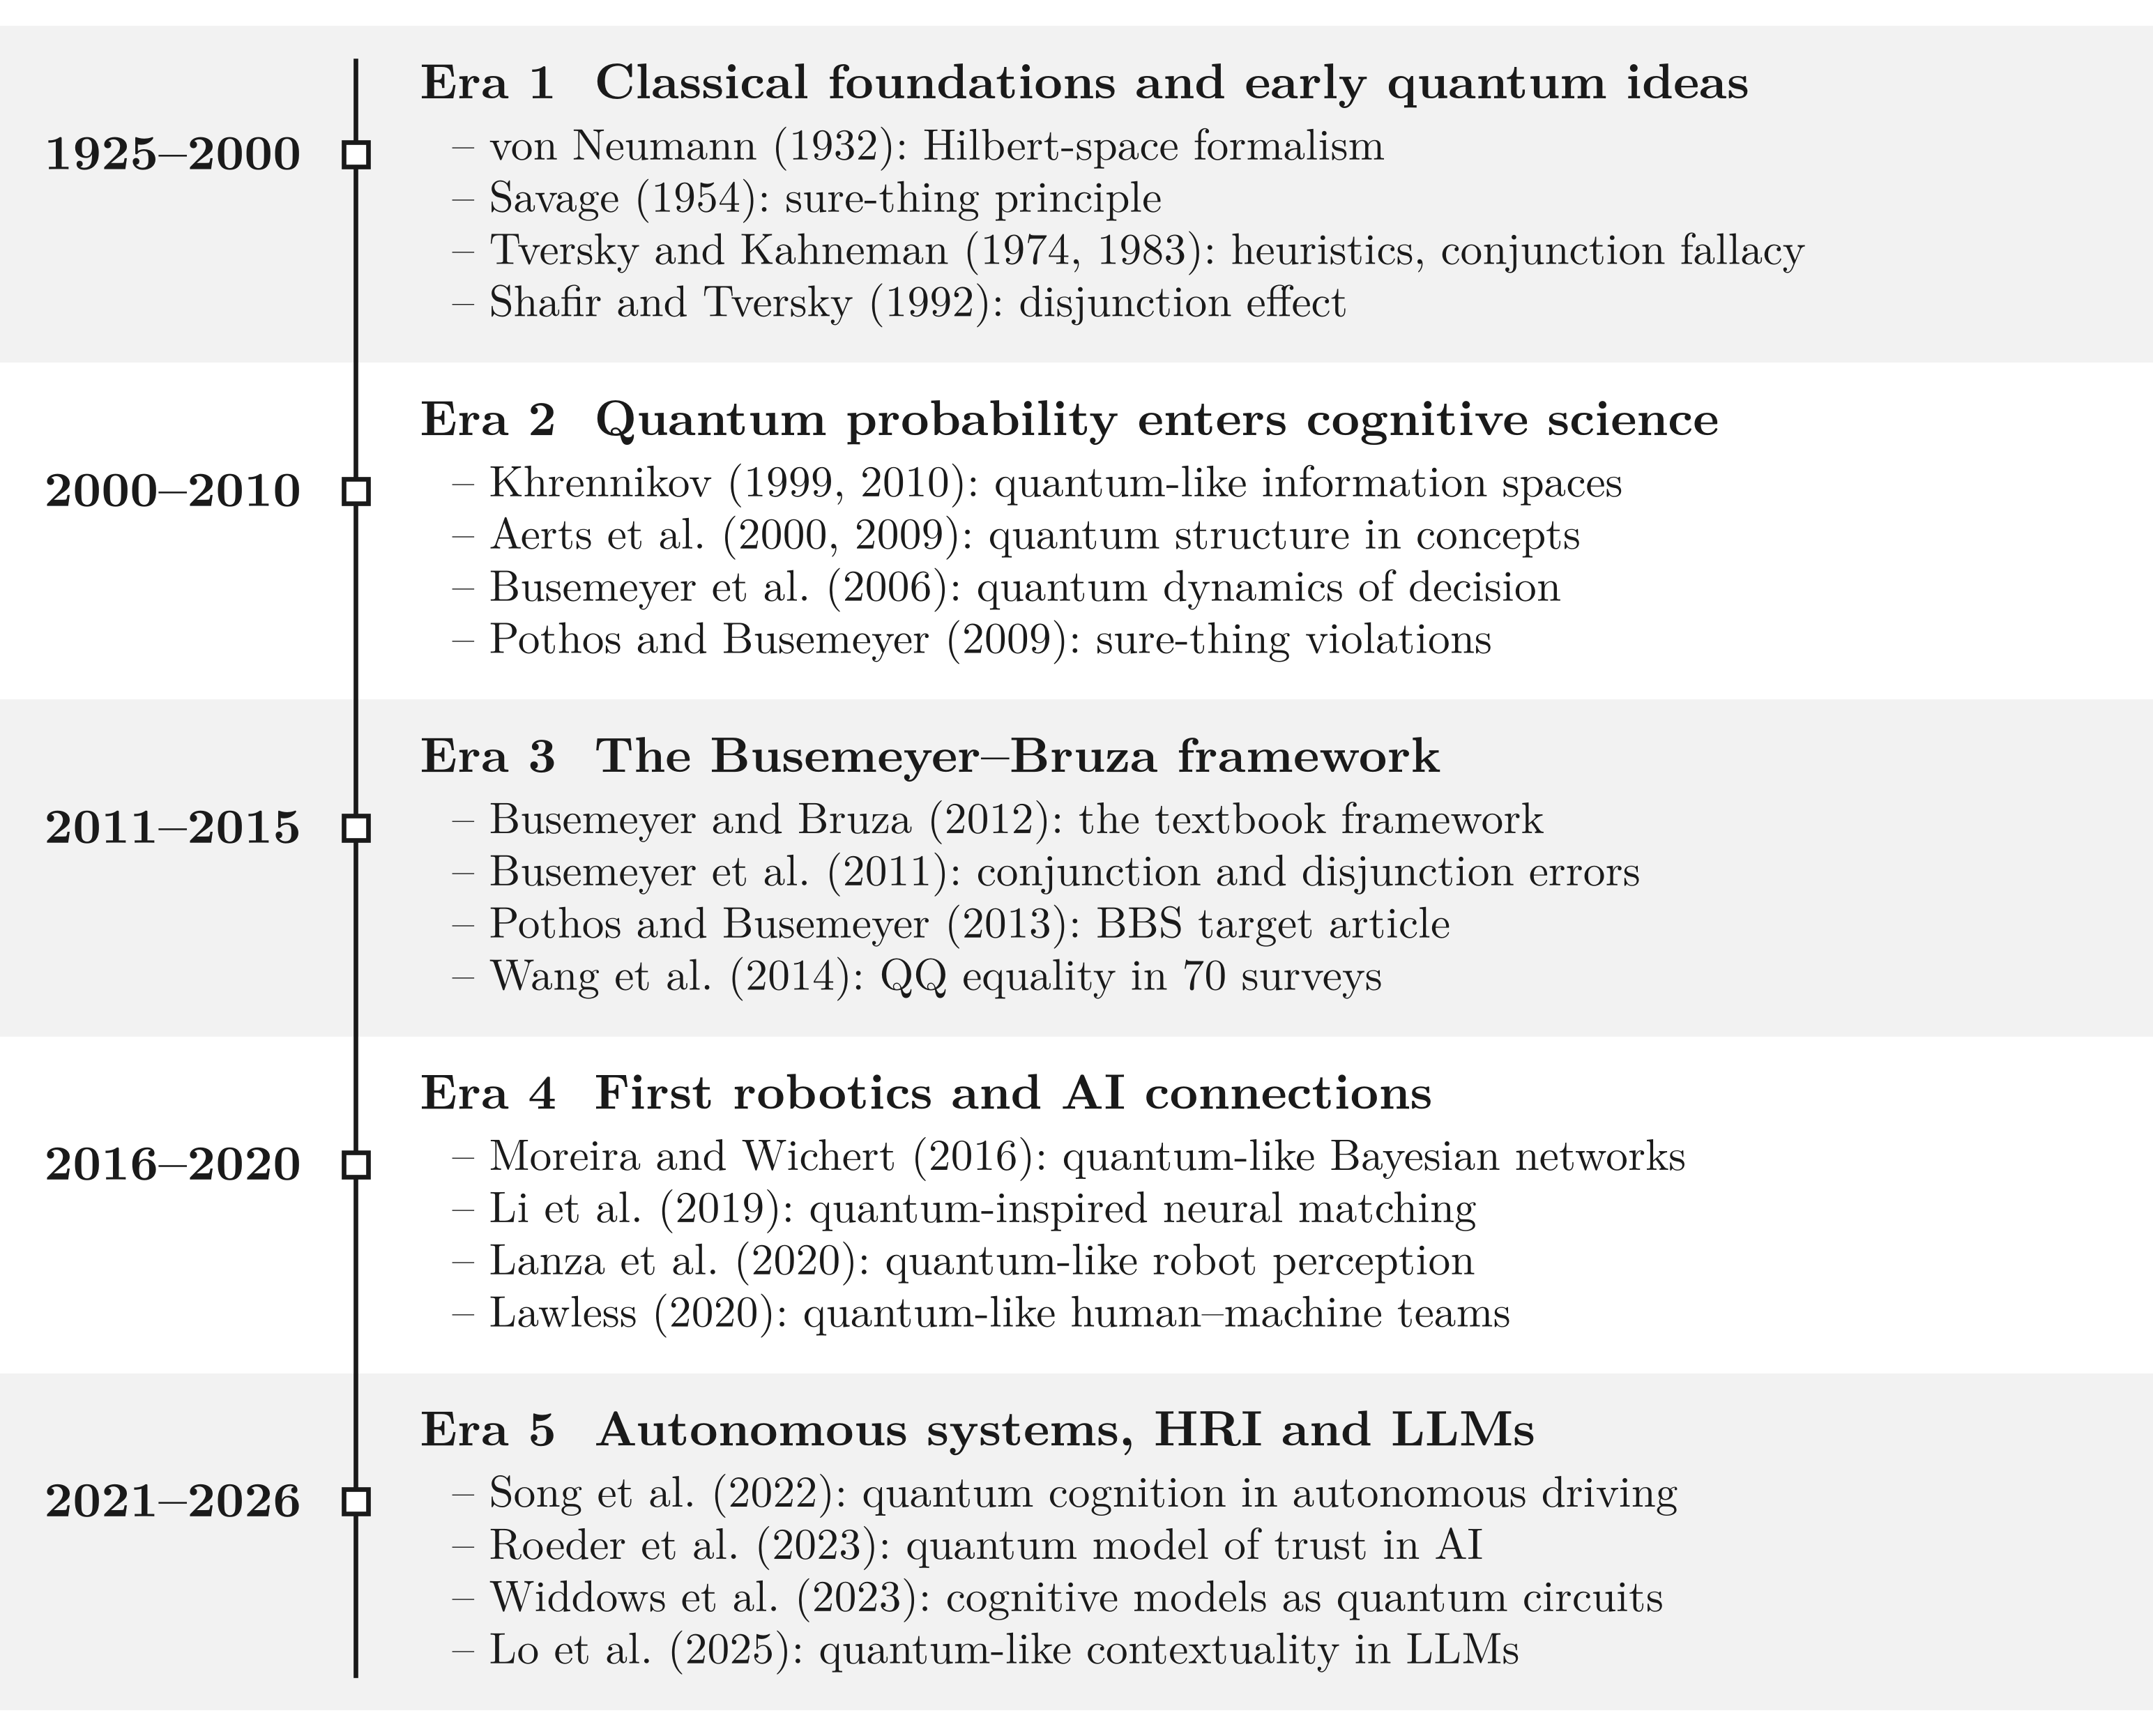
\includegraphics[width=1.00\textwidth]{figures/Fig1_eras.png}
\caption{Five eras of quantum cognition and its transfer to autonomous agents, with representative works}\label{fig:eras}
\end{figure}

\subsection{Era 1 (1925--2000): Classical Cognitive Foundations and Early Quantum Ideas}\label{sec:era1}

\subsubsection{Von Neumann and Dirac: Quantum Formalism Emerges (1925--1932)}
The formalism that quantum cognition borrows was consolidated by von Neumann, who represented states as vectors in a Hilbert space, observables as self-adjoint operators and measurement as projection~\citep{vonNeumann1932}. Two of his results matter here. First, quantum probability is defined on a lattice of subspaces that is not distributive, so the classical identity $P(A) = P(A \wedge B) + P(A \wedge \neg B)$ can fail. Second, measurement changes the state, the property later exploited to model the constructive nature of human judgement.

\subsubsection{Classical Cognitive Revolution (1950s--1980s): Bayesian Networks and Symbols}
Savage's axiomatisation of subjective expected utility made the sure-thing principle a pillar of rational choice~\citep{Savage1954}. Cognitive science then developed along two lines that still shape autonomous systems: symbolic architectures, from which today's cognitive architectures descend~\citep{Kotseruba2020,Laird2017}, and probabilistic models, later formalised as Bayesian networks and probabilistic robotics~\citep{Thrun2005}. Both assume that all variables can be placed in one sample space.

\subsubsection{Tversky and Kahneman: Decision Anomalies Surface (1974--2000)}
The heuristics-and-biases programme documented systematic departures from probability theory~\citep{Tversky1974}. The conjunction fallacy (judging ``bank teller and feminist'' more probable than ``bank teller'')~\citep{Tversky1983}, ambiguity aversion in the Ellsberg paradox~\citep{Ellsberg1961} and the disjunction effect in the Prisoner's Dilemma~\citep{Shafir1992} became the benchmark phenomena that quantum models would later address.

\subsection{Era 2 (2000--2010): Quantum Probability Enters Cognitive Science}\label{sec:era2}

\subsubsection{Aerts and Gabora: First Quantum Cognition Papers}
The Brussels group argued that concepts behave like quantum entities whose meaning is actualised by context. Aerts, D'Hondt and Gabora showed that the quantum-logical disjunction is not classical~\citep{Aerts2000}, and Aerts later showed that membership judgements for combined concepts (the ``guppy effect'' and over- and underextension) are incompatible with classical models but reproduced in Fock space~\citep{Aerts2009}.

\subsubsection{Khrennikov: Quantum-Like Formalism in Cognition}
Khrennikov developed quantum-like models of information spaces~\citep{Khrennikov1999} and a contextual probability framework in which interference arises from incompatible contexts rather than physical quantum effects~\citep{Khrennikov2010}. The ``quantum-like'' label used throughout this review originates in this work.

\subsubsection{Early Applications: Prisoner's Dilemma, Concept Combinations}
Busemeyer, Wang and Townsend introduced quantum dynamics of decision-making, contrasting quantum and Markov random walks~\citep{Busemeyer2006}. Pothos and Busemeyer then showed that interference between the ``opponent defects'' and ``opponent cooperates'' branches reproduces the disjunction effect that classical models cannot~\citep{Pothos2009}, and Busemeyer, Wang and Lambert-Mogiliansky derived parameter-free empirical tests separating Markov and quantum models~\citep{Busemeyer2009}. Bruza and colleagues asked whether the human mental lexicon is quantum-like~\citep{Bruza2009}.

\subsection{Era 3 (2011--2015): The Busemeyer and Bruza Framework Emerges}\label{sec:era3}

\subsubsection{Busemeyer and Bruza, ``Quantum Models of Cognition and Decision'' (2012)}
The monograph by Busemeyer and Bruza unified the field's principles, models and data~\citep{Busemeyer2012}; it remains the standard reference, and a second edition appeared in 2024. Its companion target article in Behavioral and Brain Sciences, with open peer commentary, made the case to mainstream cognitive science~\citep{Pothos2013a}.

\subsubsection{Order Effects and Conjunction Fallacy Formalised}
Busemeyer, Pothos, Franco and Trueblood explained conjunction and disjunction errors as sequential projections~\citep{Busemeyer2011}; Trueblood and Busemeyer modelled order effects in inference~\citep{Trueblood2011}; and Wang and Busemeyer derived the QQ equality~\citep{Wang2013b}, confirmed in 70 national surveys~\citep{Wang2014}.

\subsubsection{Interference Effects: Two-Stage Measurements in Decisions}
Two-stage paradigms, in which an intermediate judgement is either elicited or not, became the main test of interference. Making a categorisation before an action~\citep{Wang2016}, or a choice before a confidence rating~\citep{Kvam2015}, changed later judgements in ways that violate the law of total probability.

\subsubsection{Widespread Adoption in Psychology (Special Issues, Conferences)}
A special issue of Topics in Cognitive Science set out the case for quantum models of cognition~\citep{Wang2013a} and extended them to similarity~\citep{Pothos2013b}, vagueness~\citep{Blutner2013} and concept dynamics~\citep{Aerts2013}. The Quantum Interaction conference series provided a venue shared with information retrieval and AI, where the first explicit bridge to AI and robotics was proposed~\citep{Aerts2011d,Aerts2011b}. Survey articles consolidated the field~\citep{Ashtiani2015,Bruza2015}.

\subsection{Era 4 (2016--2020): Beyond Psychology --- First Robotics and AI Connections}\label{sec:era4}

\subsubsection{Quantum Cognition Applied to Autonomous Systems and ML}
Quantum-like Bayesian networks replaced classical probabilities with complex amplitudes and gave decision-support systems a way to represent sure-thing violations~\citep{Moreira2016,Moreira2017a}. In information retrieval and NLP, density-matrix language models~\citep{Sordoni2013} led to quantum-inspired neural networks for matching and sentiment~\citep{Zhang2018,Li2019}. In RL, a separate line of quantum-inspired algorithms had already been validated on a mobile robot~\citep{Dong2008,Dong2012}, and projective simulation offered a physics-motivated learning agent~\citep{Briegel2012} tested on real robotic manipulation~\citep{Hangl2016}. Order effects were proposed as a design concern for the queries of intelligent agents~\citep{Kak2018}.

\subsubsection{Exploration of Sensor Fusion and Perception Problems}
Quantum-inspired multimodal fusion treated modalities as incompatible measurement contexts~\citep{Li2021a,Gkoumas2021}. For robots, Lanza, Solinas and Mastrogiovanni proposed a quantum-like perception model in which percepts are qubit states and queries are measurements~\citep{Lanza2020}, extended to multi-sensory integration~\citep{Lanza2021}.

\subsubsection{Hybrid Quantum-Classical Architectures for Real-Time Control}
Early ``quantum robot'' architectures combined classical controllers with (then hypothetical) quantum processors~\citep{Benioff1998,Dong2006}; robot emotion was modelled as a qubit-encoded emotion space~\citep{Yan2019} and as mixed states of reflection and affect~\citep{Hoorn2019}; and a quantum-like cognitive architecture was proposed as an alternative to resource-rational analysis~\citep{Moreira2020a}. None of these architectures closed a real-time control loop with a quantum processor.

\subsection{Era 5 (2021--Present): Quantum Cognition for Autonomous Systems}\label{sec:era5}

\subsubsection{Fault Diagnosis and Multi-Goal Trade-offs in Autonomous Robots}
Recent robot-facing work includes quantum-like pedestrian-intention models for automated driving~\citep{Song2022}, quantum affective decision models for social robots~\citep{Ho2022,Yan2021c}, quantum-circuit teleo-reactive controllers~\citep{Chella2026}, quantum game models of driving interactions~\citep{Essalmi2025,Essalmi2026} and a social-robotics research programme~\citep{DeCarolis2025}. Multi-goal trade-offs appear in quantum-like evidence networks~\citep{Gao2025} and multi-attribute decision models~\citep{She2021}. We found no study that applies quantum cognition to fault diagnosis in robots; the closest work is a fault-tolerant quantum filter for quantum systems~\citep{Gao2021}, which addresses a different problem.

\subsubsection{ML and AI Integration: Feature Learning and Decision-Making}
Quantum-cognitive fusion~\citep{Gkoumas2021}, density-matrix matching~\citep{Zhang2025} and quantum-cognitive neural networks that reproduce human-like confidence~\citep{Maksimovic2025} extend quantum-inspired ML, and complex-valued sequence models with Born-rule decoding carry the same ideas into language modelling~\citep{Nebli2026}. Since 2024, a new line probes LLMs for quantum-like structure: contextuality in LLM-derived probabilities~\citep{Lo2025}, context effects in similarity judgements~\citep{Uprety2024}, Bell-type correlations in concept combinations~\citep{Aerts2026}, and probability-judgement fallacies~\citep{Imannezhad2026,Kang2026}.

\subsubsection{RL Applications: Policy Optimisation Under Uncertainty}
Quantum-inspired experience replay continued the classical quantum-inspired RL line~\citep{Wei2022}, while variational-circuit RL grew into a separate field that the companion survey reviews~\citep{Guru2026,Meyer2022}. On the cognitive side, open-system quantum--Markov models describe how preferences and beliefs evolve~\citep{Busemeyer2020,Kvam2021,Epping2023}, and quantum models of trust in AI track how human reliance changes during interaction~\citep{Roeder2023,vanderMeer2025,Humr2025}. Both are candidate models of the human reward-giver in RL from human feedback (Section \ref{sec:mdp}).

\subsubsection{Integration with Survey 1 (Quantum Robotics Comprehensive Overview)}\label{sec:era5-s1}
This review is the second of a pair. The companion systematic survey~\citep{Guru2026} covers quantum computing, sensing and communication for robots: quantum optimisation and search for planning and scheduling, variational-circuit reinforcement learning, quantum navigation sensors and quantum communication between robots, graded by how close each result comes to a working robot. It found that no quantum-computing method has yet reached deployment on a robot, whereas quantum sensing and communication have, and it treats quantum cognition in a single short section. The present review is the in-depth treatment of the cognitive side. Quantum cognition needs no quantum processor, so its bottleneck is empirical validation rather than hardware: of the quantum routes into robotics surveyed in the two reviews, it is the only one whose claimed benefit, a better representation of human-like judgement, can be tested on robots and AI systems today. Where the two meet, for example quantum RL and circuit implementations of cognitive models, we refer to the companion survey for hardware constraints. Studies that use quantum computation only as an accelerator are excluded here (criterion E5) and cited only to mark the boundary; eight application studies are discussed in both reviews, from different angles, and are flagged in the dataset (Online Resource 3).


%% -----------------------------------------------------------------------------
\section{Mathematical Preliminaries --- Linear Algebra and Hilbert Spaces (for AI/ML/Roboticists)}\label{sec:math}
This section gives the minimum machinery needed to read the rest of the review; derivations are collected in Appendix \ref{app:math}, and tutorials are available elsewhere~\citep{Yearsley2016a,Yearsley2017}.

\subsection{Complex Vector Spaces and Inner Products}\label{sec:vec}
A state is a vector $\ket{\psi}$ in $\mathbb{C}^n$. The inner product $\langle\phi|\psi\rangle = \sum_i \phi_i^{*}\psi_i$ is linear in its second argument and conjugate-linear in its first; the norm is $\lVert\psi\rVert = \sqrt{\langle\psi|\psi\rangle}$. Complex amplitudes matter because probabilities are squared magnitudes: two paths to the same outcome add as amplitudes, and their relative phase determines whether they reinforce or cancel.

\subsection{Hilbert Spaces and Orthonormality}\label{sec:hilbert}
A Hilbert space is a complete inner-product space; all models in this review are finite-dimensional, so it is simply $\mathbb{C}^n$ with the standard inner product. An orthonormal basis $\{\ket{e_i}\}$ satisfies $\langle e_i|e_j\rangle = \delta_{ij}$. In cognitive models each basis vector represents a fully resolved answer pattern, and different questions correspond to different bases of the same space.

\subsection{Linear Operators and Matrices}\label{sec:ops}
Observables are Hermitian operators ($A = A^{\dagger}$); dynamics are unitary operators ($U^{\dagger}U = I$) that preserve norms, generated by a Hermitian Hamiltonian $H$ through $U(t) = \exp(-iHt)$. Two operators are compatible when they commute ($AB = BA$). The commutator $[A, B] = AB - BA$ measures incompatibility and is the formal source of order effects.

\subsection{Eigenvalues, Eigenvectors and Projectors}\label{sec:proj}
A Hermitian operator has real eigenvalues and an orthonormal basis of eigenvectors; each distinct answer to a question corresponds to an eigenvalue, and the eigenvectors with that eigenvalue span the answer's subspace. A projector $P$ satisfies $P = P^{\dagger} = P^2$; it projects onto that subspace. The Born rule gives $p(\text{answer}) = \lVert P\ket{\psi}\rVert^2 = \bra{\psi}P\ket{\psi}$, and the L\"uders rule gives the post-answer state $P\ket{\psi}/\lVert P\ket{\psi}\rVert$. Sequential judgements therefore have probability $p(A \text{ then } B) = \lVert P_B P_A \ket{\psi}\rVert^2$, which differs from $p(B \text{ then } A)$ when $P_A$ and $P_B$ do not commute. Mixed states are density matrices $\rho$ (positive, unit trace), with $p = \mathrm{tr}(P\rho)$; general measurements are positive-operator-valued measures (POVMs) or quantum instruments, which are needed to model some combinations of effects (Section \ref{sec:postulates})~\citep{Ozawa2020,Fuyama2025}.

\subsection{Tensor Products and Multi-Dimensional Spaces}\label{sec:tensor}
Composite systems live in tensor products: two binary questions that are compatible can be represented in $\mathbb{C}^2 \otimes \mathbb{C}^2 = \mathbb{C}^4$. States that cannot be written as products (entangled states) represent dependencies that are not reducible to separate beliefs, and have been used to model concept combination~\citep{Aerts2011a}. For ML practitioners, tensor products are also the basis of tensor-network models~\citep{Stoudenmire2016}. The dimension grows as $2^n$ for $n$ binary variables, which is the central computational limitation of naive QP models (Section \ref{sec:hw}). Hilbert-space multidimensional theory addresses this by choosing low-dimensional representations tailored to the questions asked~\citep{Busemeyer2018}.


%% -----------------------------------------------------------------------------
\section{Standardised Terminology --- Glossary and Visual Diagrams}\label{sec:terminology}

\subsection{Key Terms: Superposition, Entanglement, Interference, Measurement}\label{sec:terms}
In quantum cognition these terms are used in a precise mathematical sense that should not be confused with claims about physical quantum states in the brain. Superposition denotes a state that is a linear combination of answer states, representing unresolved uncertainty that is not mere ignorance of a fixed answer. Measurement is the act of eliciting a judgement or decision, which projects the state and so changes subsequent judgements. Interference is the cross term that appears when the probability of an outcome is computed from two unresolved paths; it is responsible for violations of the law of total probability. Entanglement is non-separability of a composite state; in cognition it is usually diagnosed by Bell-type or CHSH inequalities, and such diagnoses require care because signalling between measurements (direct influence of context on marginal probabilities) can mimic it~\citep{Dzhafarov2016a}.

\subsection{Quantum vs. Classical Probability}\label{sec:qvc}
Table \ref{tab:qvc} compares the two frameworks. Classical probability assigns probabilities to subsets of one sample space and is commutative and distributive; QP assigns them to subspaces, is non-commutative for incompatible questions and violates the distributive law. Both satisfy the basic axioms for a single set of compatible events, and QP reduces to classical probability when all projectors commute~\citep{Bruza2015}. The difference matters only for incompatible questions, which is why careful experimental design is needed to discriminate the two.

\begin{table}[ht]
\caption{Classical versus quantum probability}\label{tab:qvc}%
\footnotesize
\begin{tabular}{@{}>{\raggedright\arraybackslash}p{0.240\dimexpr\textwidth-6\tabcolsep\relax}>{\raggedright\arraybackslash}p{0.360\dimexpr\textwidth-6\tabcolsep\relax}>{\raggedright\arraybackslash}p{0.400\dimexpr\textwidth-6\tabcolsep\relax}@{}}
\toprule
\textbf{Aspect} & \textbf{Classical (Kolmogorov) probability} & \textbf{Quantum probability} \\ \midrule
Events & Subsets of one sample space & Subspaces of a Hilbert space \\
State & Probability distribution & Unit vector $\ket{\psi}$ or density matrix $\rho$ \\
Probability rule & Measure of the subset & Born rule: $\lVert P\ket{\psi}\rVert^2$ or $\mathrm{tr}(P\rho)$ \\
Updating & Bayes' rule (conditioning) & L\"uders rule (projection) or quantum instrument \\
Conjunction & Commutative & Sequential and order-dependent for incompatible questions \\
Law of total probability & Always holds & Can be violated by interference terms \\
Distributive law & Holds & Fails for incompatible events \\
Joint distribution & Always exists & Exists only for compatible questions \\
Dynamics & Markov (Kolmogorov) equations & Unitary (Schr\"odinger) or open-system (Lindblad) equations \\
Relation & -- & Reduces to classical probability when all projectors commute \\
\botrule
\end{tabular}
\end{table}

\subsection{Visual Diagrams: Bloch Sphere, State Vectors, Measurement Bases}\label{sec:diagrams}
Figure \ref{fig:order} illustrates the geometry of an order effect and Figure \ref{fig:bloch} the standard geometric picture for a single binary question; interference is illustrated in Figure \ref{fig:interference} (Section \ref{sec:interference}). On the Bloch sphere, a pure state of one qubit is a point on the surface; a binary question is a diameter; the probability of ``yes'' is $\cos^2(\theta/2)$, where $\theta$ is the angle between the state and the ``yes'' pole. Two questions whose diameters are not aligned are incompatible.

\begin{figure}[ht]
\centering
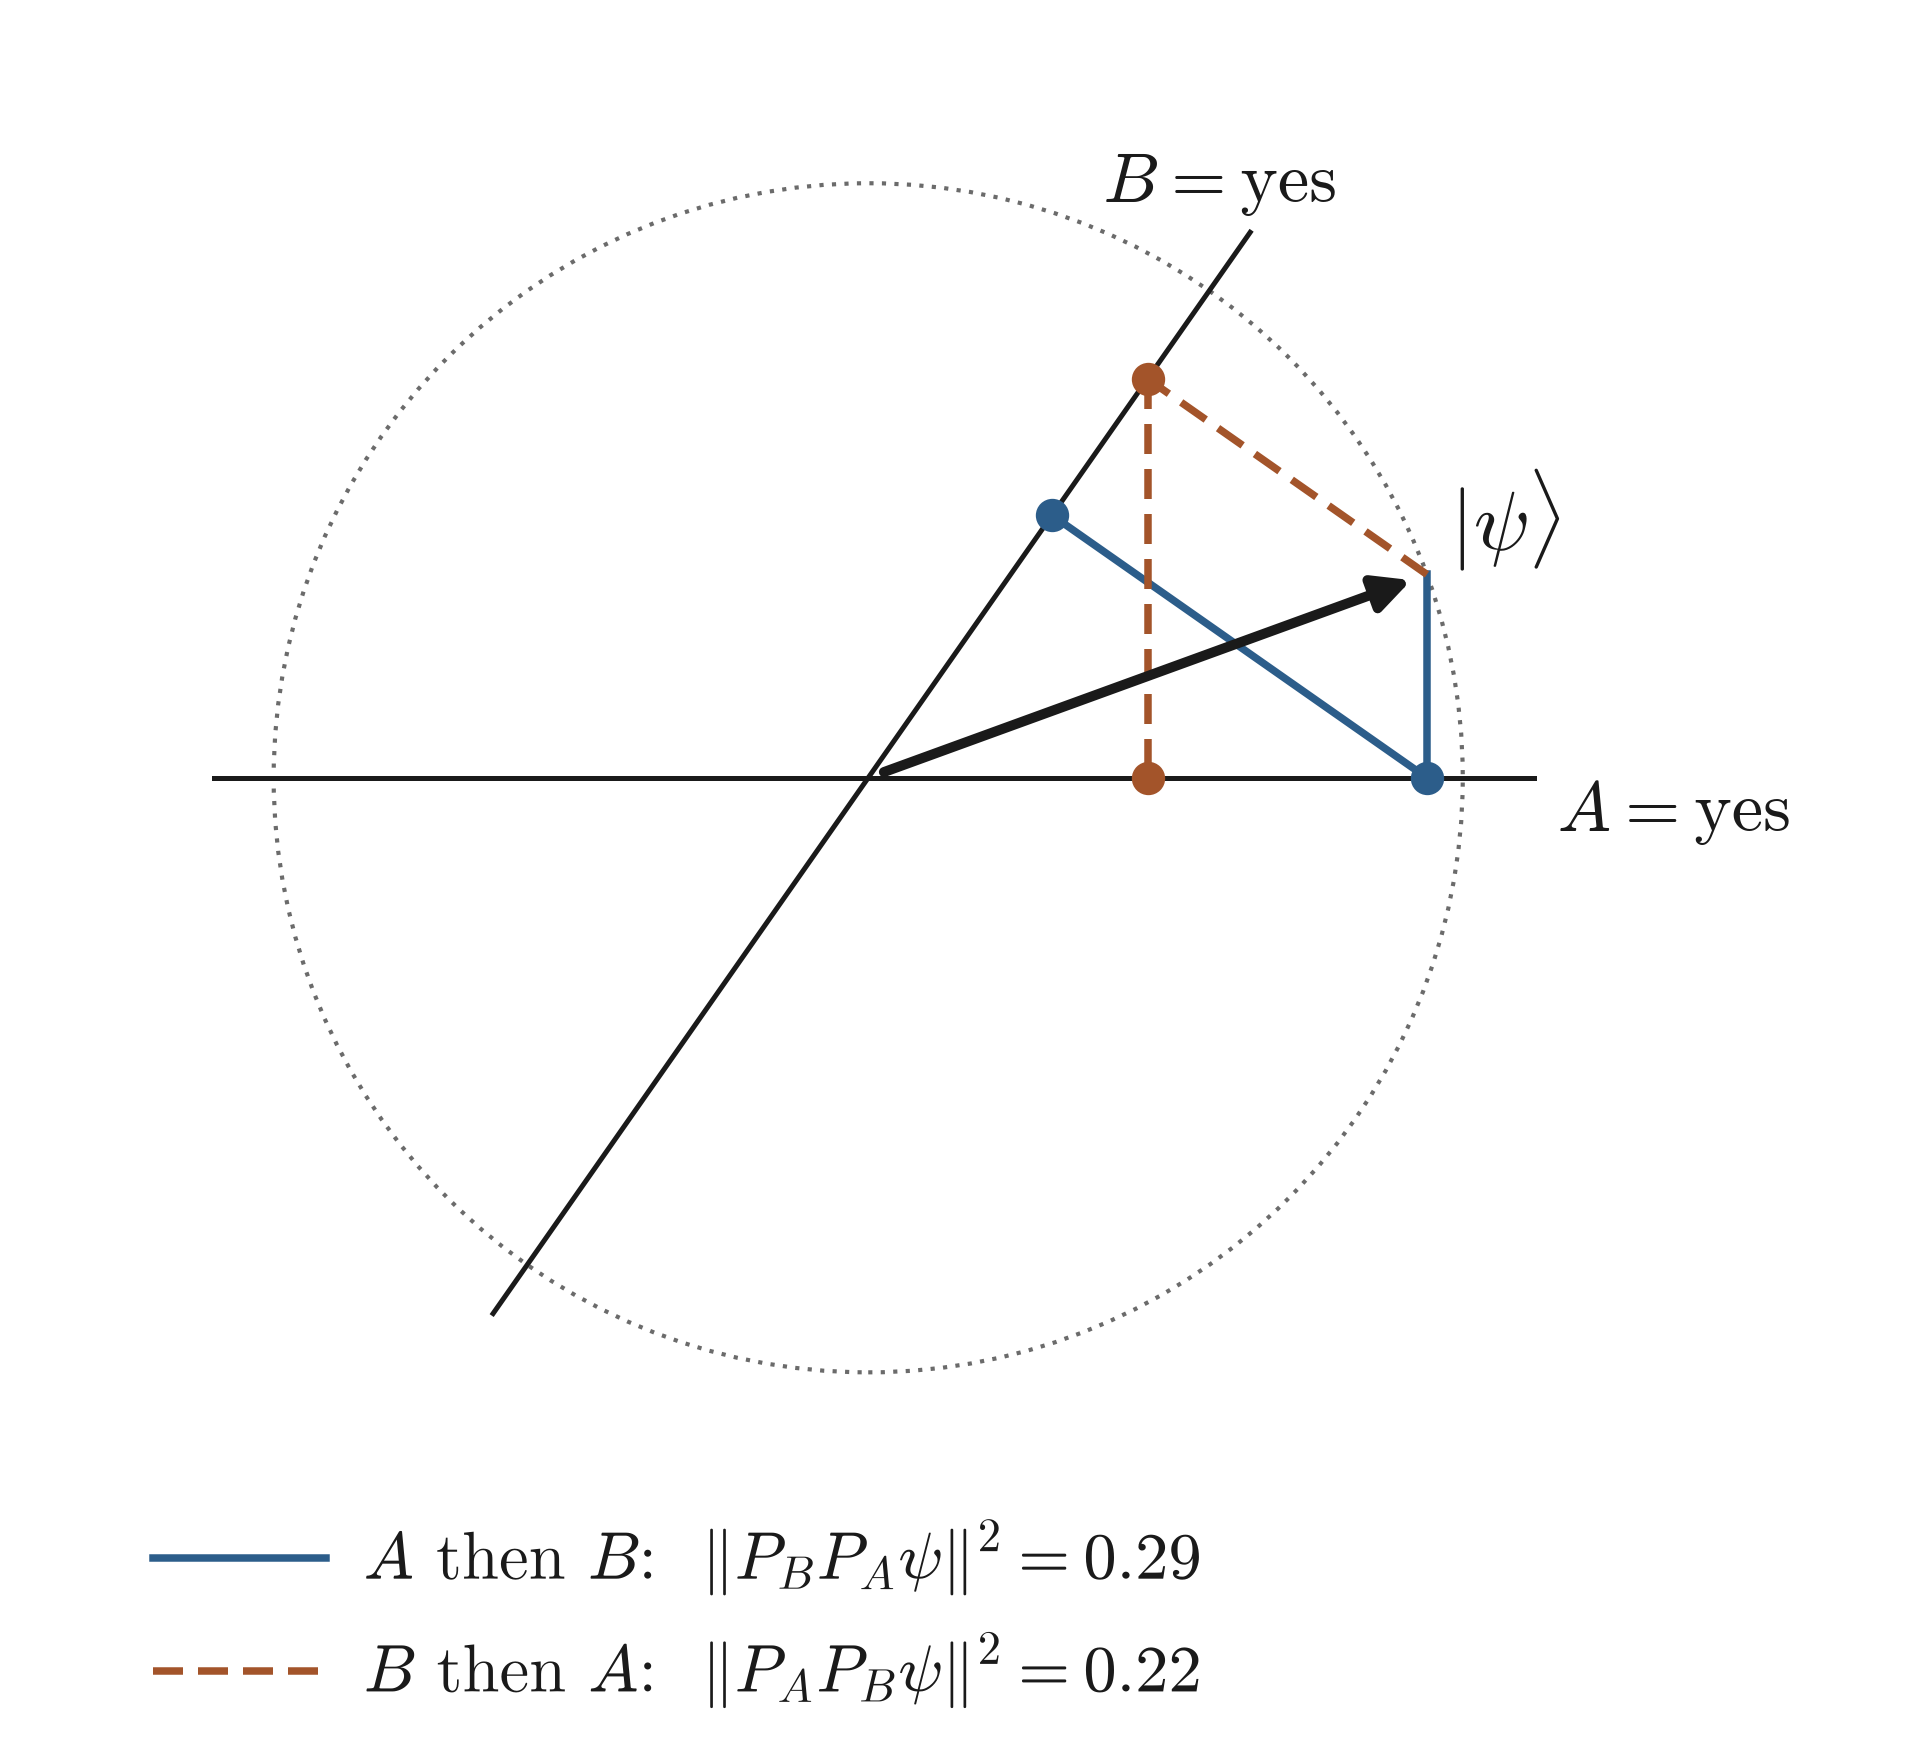
\includegraphics[width=0.62\textwidth]{figures/Fig2_order_geometry.png}
\caption{Geometry of a question-order effect in a real two-dimensional belief space. The state $\ket{\psi}$ is projected onto ``A = yes'' then ``B = yes'' (solid path) or in the reverse order (dashed path). With the angles used in Example 1 (Section \ref{sec:order}), $p(A \text{ then } B) = 0.29$ and $p(B \text{ then } A) = 0.22$, while the QQ equality is satisfied exactly}\label{fig:order}
\end{figure}

\begin{figure}[ht]
\centering
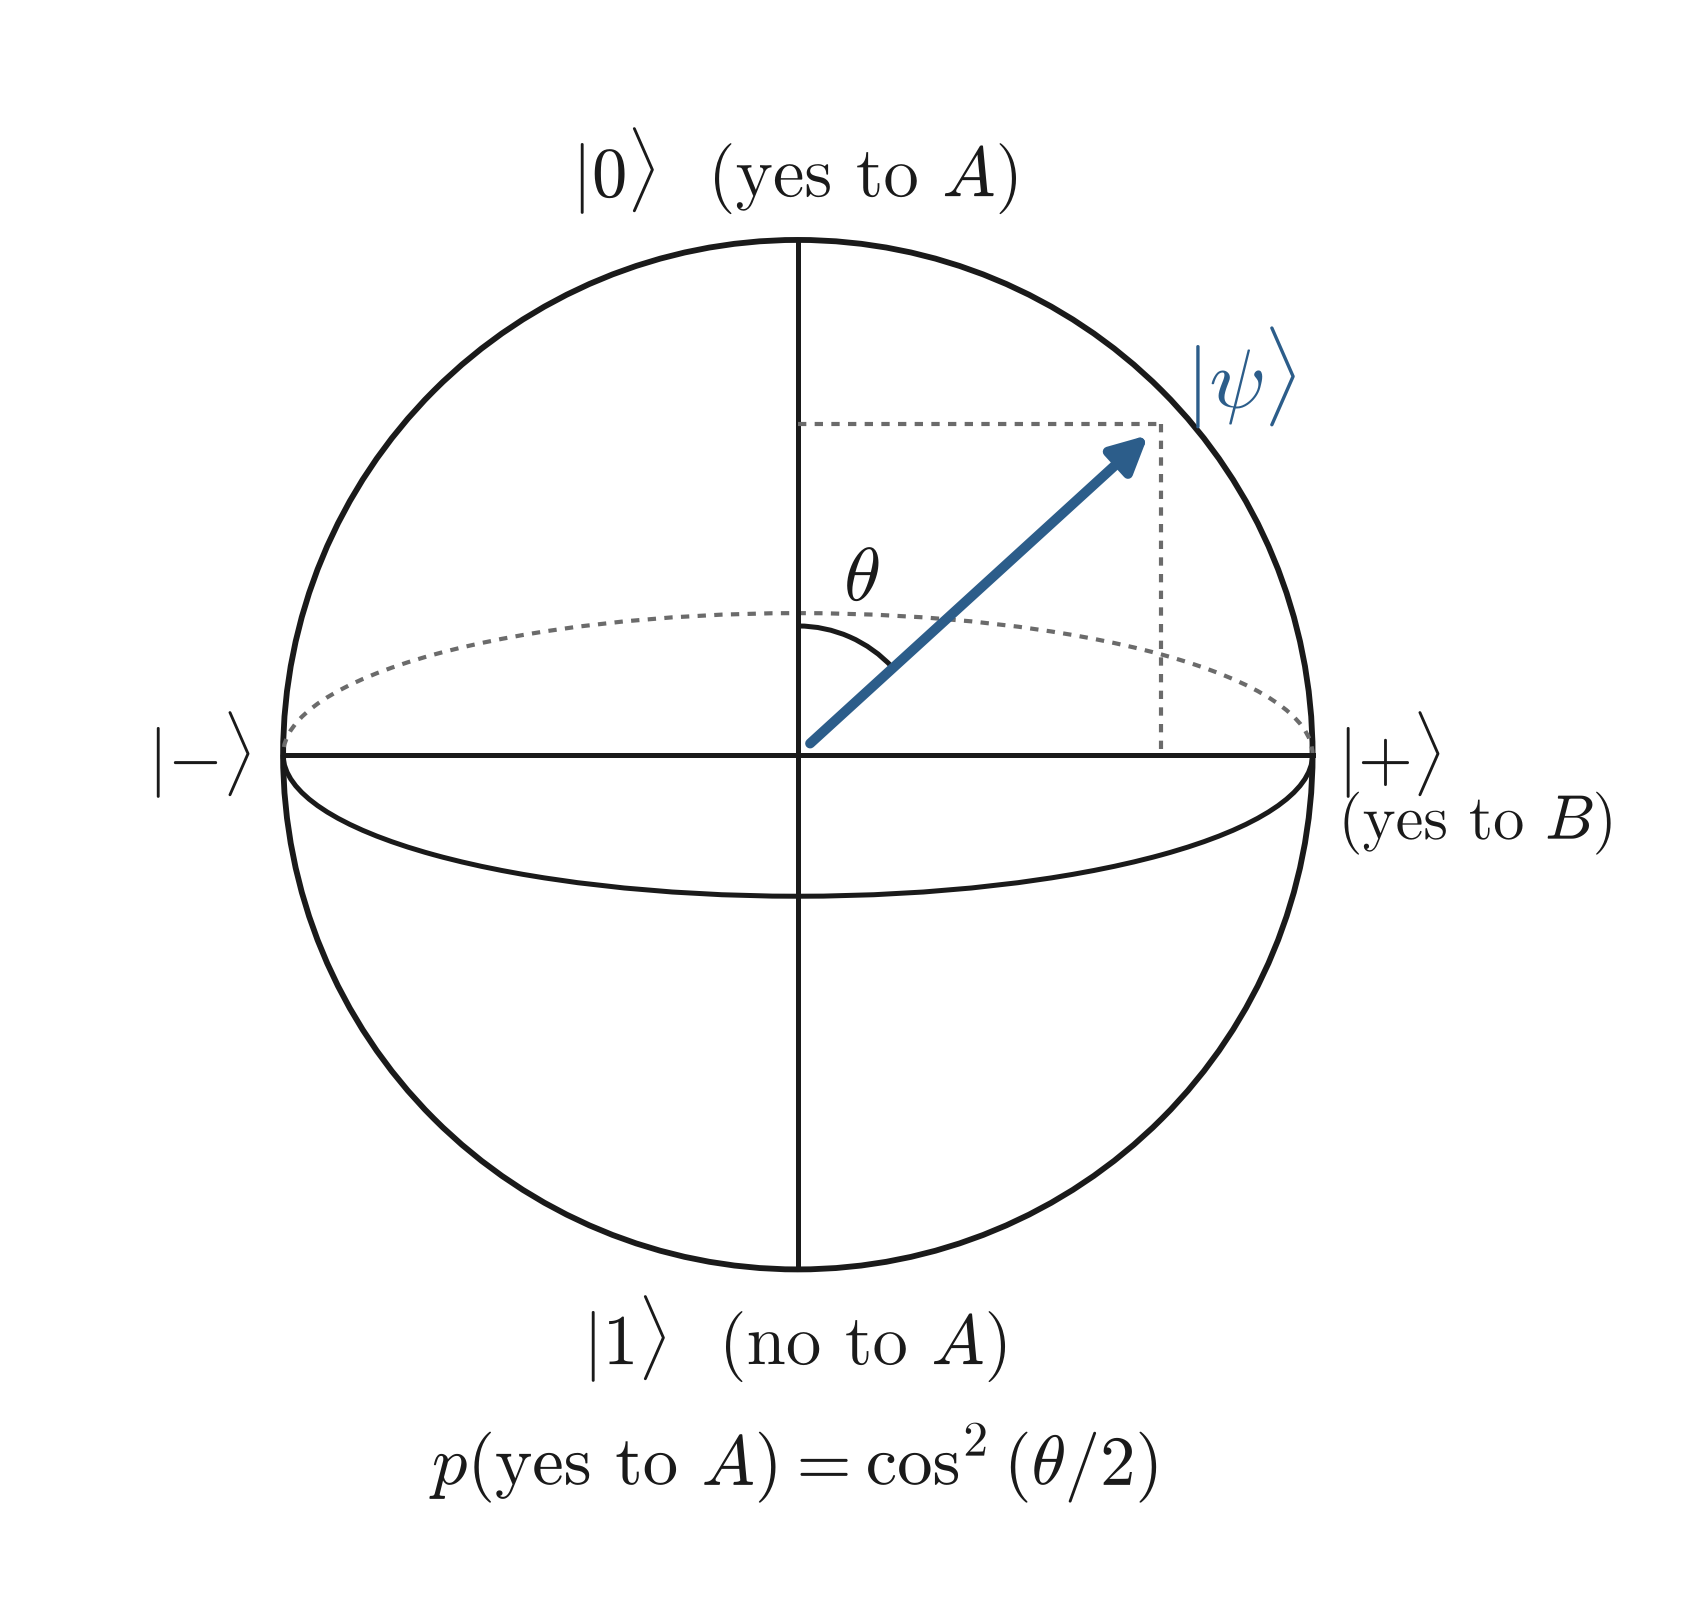
\includegraphics[width=0.55\textwidth]{figures/Fig3_bloch.png}
\caption{Bloch-sphere representation of a single binary judgement. Complementary questions A and B correspond to orthogonal axes; the state $\ket{\psi}$ has definite probabilities for both, but no joint distribution over the two answers}\label{fig:bloch}
\end{figure}

\subsection{Glossary of Symbols and Notation}\label{sec:glossary}
Table \ref{tab:glossary} lists the symbols and abbreviations used in the review.

\begin{table}[ht]
\caption{Glossary of symbols and notation}\label{tab:glossary}%
\footnotesize
\begin{tabular}{@{}>{\raggedright\arraybackslash}p{0.300\dimexpr\textwidth-4\tabcolsep\relax}>{\raggedright\arraybackslash}p{0.700\dimexpr\textwidth-4\tabcolsep\relax}@{}}
\toprule
\textbf{Symbol} & \textbf{Meaning} \\ \midrule
$\ket{\psi}$, $\bra{\psi}$ & State vector (ket) and its conjugate transpose (bra) \\
$\langle\phi|\psi\rangle$ & Inner product \\
$\rho$ & Density matrix (mixed state); $\mathrm{tr}\,\rho = 1$, $\rho \succeq 0$ \\
$P_A$, $I - P_A$ & Projectors onto the ``yes'' and ``no'' subspaces of question A \\
$[A, B] = AB - BA$ & Commutator; zero for compatible questions \\
$\lVert P\ket{\psi}\rVert^2$ & Born-rule probability \\
$U(t) = \exp(-iHt)$ & Unitary evolution generated by Hamiltonian $H$ \\
$L_k$, $\gamma_k$ & Lindblad (jump) operators and rates in open-system models \\
$\otimes$ & Tensor product of spaces or states \\
$\theta$ & Interference phase between two branches \\
QQ & Quantum question equality \\
QLBN & Quantum-like Bayesian network \\
QRL, QiRL & Quantum and quantum-inspired reinforcement learning \\
PQC, VQC & Parametrised and variational quantum circuit \\
PS & Projective simulation \\
CbD & Contextuality-by-default \\
POVM & Positive-operator-valued measure (generalised measurement) \\
QPU & Quantum processing unit \\
\botrule
\end{tabular}
\end{table}


%% =============================================================================
\surveypart{Part B --- Theory (Sections 5--7)}

\section{Foundational Theory --- Busemeyer, Bruza, Order Effects, Conjunction Fallacy}\label{sec:theory}

\subsection{Overview of Quantum Cognition as a Psychological Theory}\label{sec:psych}
Quantum cognition is best understood as a family of formal models, not a single theory of mind. Its common core is the use of QP to represent judgement and decision processes in which the act of judging is constructive: a person does not read out a pre-existing answer but creates one in the context of the question, and that answer becomes part of the context for the next question~\citep{Busemeyer2012,Pothos2013a}. On this view the probabilistic ``errors'' catalogued by the heuristics-and-biases programme are not failures of a classical reasoner but signatures of a different, and arguably principled, probability calculus~\citep{Pothos2017}. The Annual Review by Pothos and Busemeyer~\citep{Pothos2022} and the 2025 overview of the research programme~\citep{Huang2025b} are the authoritative summaries; Busemeyer and Wang give an accessible introduction~\citep{Busemeyer2015}.

\subsection{The Quantum Cognition Framework: Core Postulates}\label{sec:postulates}
Following~\citet{Busemeyer2012} and~\citet{Yearsley2016a}, a quantum cognitive model specifies five elements:

\begin{itemize}
\item A Hilbert space whose dimension is set by the number of distinguishable answer patterns (often 2--4 dimensions per question set).
\item An initial belief state $\ket{\psi}$ (or density matrix $\rho$) before any question is asked.
\item A projector (or, more generally, an instrument) for each answer to each question, with incompatible questions represented in different bases.
\item Born and L\"uders rules for the probability of an answer and the updated state.
\item Optionally, a Hamiltonian or Lindblad generator for how the state evolves between measurements, for example as evidence accumulates~\citep{Busemeyer2006,Busemeyer2020}.
\end{itemize}

Two refinements are now standard. First, projective measurement alone cannot reproduce both question-order effects and response replicability (repeating a question returns the same answer), a result known as the response-replicability problem~\citep{Khrennikov2014}. Quantum instruments, more general state-update maps, resolve this~\citep{Ozawa2020,Ozawa2021}, and recent work argues that the non-classicality of cognition lies in non-commuting state updates rather than non-commuting observables~\citep{Fuyama2025,Busemeyer2025}. Second, pure unitary dynamics predicts perpetual oscillation, so open-system (quantum--Markov, Gorini--Kossakowski--Sudarshan--Lindblad) models, in which the belief state couples to an environment and settles into a decision, have become the preferred dynamical framework~\citep{Busemeyer2020,Khrennikov2023a,Asano2026}. These refinements increase flexibility and thus the burden of showing that a model is not merely descriptive (Section \ref{sec:limits})~\citep{Broekaert2017}.

\subsection{Order Effects: Why Measurement Sequence Matters}\label{sec:order}
If the questions ``Is Clinton honest?'' and ``Is Gore honest?'' are represented by non-commuting projectors $P_A$ and $P_B$, then $p(A\text{ yes, then }B\text{ yes}) = \lVert P_B P_A \psi\rVert^2$ differs from $p(B\text{ yes, then }A\text{ yes})$. Wang and Busemeyer showed that any such model, as long as the questions are represented by projectors and the state is pure, obeys a parameter-free constraint, the QQ equality: $[p(A_yB_n) + p(A_nB_y)] - [p(B_yA_n) + p(B_nA_y)] = 0$~\citep{Wang2013b}. Classical Markov models that produce order effects do not generally satisfy it. Wang, Solloway, Shiffrin and Busemeyer tested the equality in 70 national surveys on question order and found it statistically supported, while anchoring-and-adjustment models failed to reproduce the pattern~\citep{Wang2014}. Order effects also arise in inference, where evidence presented in different orders leads to different final beliefs~\citep{Trueblood2011,Trueblood2017a}.

Worked Example 1 makes the mechanism concrete (code in Appendix \ref{app:code} and Online Resource 2). Take a real two-dimensional belief space with the state at 20\textdegree{}, question A at 0\textdegree{} and question B at 55\textdegree{}. Then $p(A\text{ yes}) = 0.883$ and $p(B\text{ yes}) = 0.671$; $p(A\text{ yes, then }B\text{ yes}) = 0.291$ while $p(B\text{ yes, then }A\text{ yes}) = 0.221$, an order effect of 7 percentage points; and the QQ quantity evaluates to zero to machine precision (Figure \ref{fig:order}). The effect disappears exactly when the projectors commute: here the norm of their commutator is 0.66, and setting the two angles equal or orthogonal reduces it to zero.

Two cautions apply. The QQ equality is necessary rather than sufficient evidence for a quantum model: non-Hilbertian and classical models can also satisfy it~\citep{Aerts2017b,Kellen2018}, and when interference plays no role the same order effects can be captured by a classical projection model~\citep{Moreira2017b}. The claim therefore rests on the combination of an a priori prediction and its robust confirmation, not on uniqueness.

\subsection{The Conjunction Fallacy: Violations of Classical Probability}\label{sec:conj}
In the classic Linda problem, people judge ``Linda is a feminist bank teller'' more likely than ``Linda is a bank teller''~\citep{Tversky1983}. The quantum account treats the conjunction as a sequence of projections: judging the more representative property first (``feminist'') moves the state towards a subspace from which ``bank teller'' is more reachable than from the initial state~\citep{Busemeyer2011}. Worked Example 2 shows this. With the state at 0\textdegree{}, ``feminist'' at 40\textdegree{} and ``bank teller'' at 80\textdegree{}, $p(\text{bank teller}) = 0.030$ but $p(\text{feminist, then bank teller}) = 0.344$, so the model produces a large conjunction fallacy without any free parameter beyond the three angles. The same model predicts disjunction errors and the relative size of both effects~\citep{Busemeyer2011}.

The conjunction fallacy is also where the quantum account is most contested. Boyer-Kassem, Duch\^ene and Guerci derived testable consequences of the main quantum-like models and found experimental results at odds with them~\citep{BoyerKassem2016}; web-scale tests suggest that emergent meaning in concept combination, rather than order, drives the effect~\citep{Aerts2017}; and the ``probability theory plus noise'' model explains conjunction and related biases with noisy classical reasoning~\citep{Costello2014,Costello2018}. A review of experimental designs shows that most studies have explored a narrow part of the possible outcome space~\citep{Veloz2024}. For autonomous systems, the practical conclusion is that conjunction-fallacy modelling alone is weak justification for adopting QP.

\subsection{Interference Effects: Double-Slit Analogy in Decision-Making}\label{sec:interference}
In the double-slit experiment, the pattern produced when the path is unobserved is not the sum of the patterns for each path. The decision analogue is the disjunction effect. In a one-shot Prisoner's Dilemma, Shafir and Tversky found that 97\% of participants defected when told the opponent had defected and 84\% when told the opponent had cooperated, but only 63\% when the opponent's move was unknown~\citep{Shafir1992}. The law of total probability requires the unknown case to lie between 0.84 and 0.97 (0.905 with equal priors). In QP the unknown-case probability is the classical mixture plus an interference term $2\sqrt{\pi_1 p_1 \pi_2 p_2}\cos\theta$, where $\pi_1$ and $\pi_2$ are the prior weights of the two branches (Appendix \ref{app:interf}). Worked Example 3 solves for this term (Figure \ref{fig:interference}): the observed 0.63 requires an interference term of $-0.275$, which corresponds to a phase $\theta \approx 108$\textdegree{}~\citep{Pothos2009}. The model explains the violation, but in this form the phase is fitted to the very datum it explains, which is why later work has sought ways to predict it, as discussed in Section \ref{sec:fusion}~\citep{Moreira2016,Wichert2020}. Yukalov and Sornette's quantum decision theory provides an alternative formalism in which an ``attraction factor'' plays the role of interference and a quarter-law gives an a priori estimate of its size~\citep{Yukalov2011,Yukalov2016}.

\begin{figure}[ht]
\centering
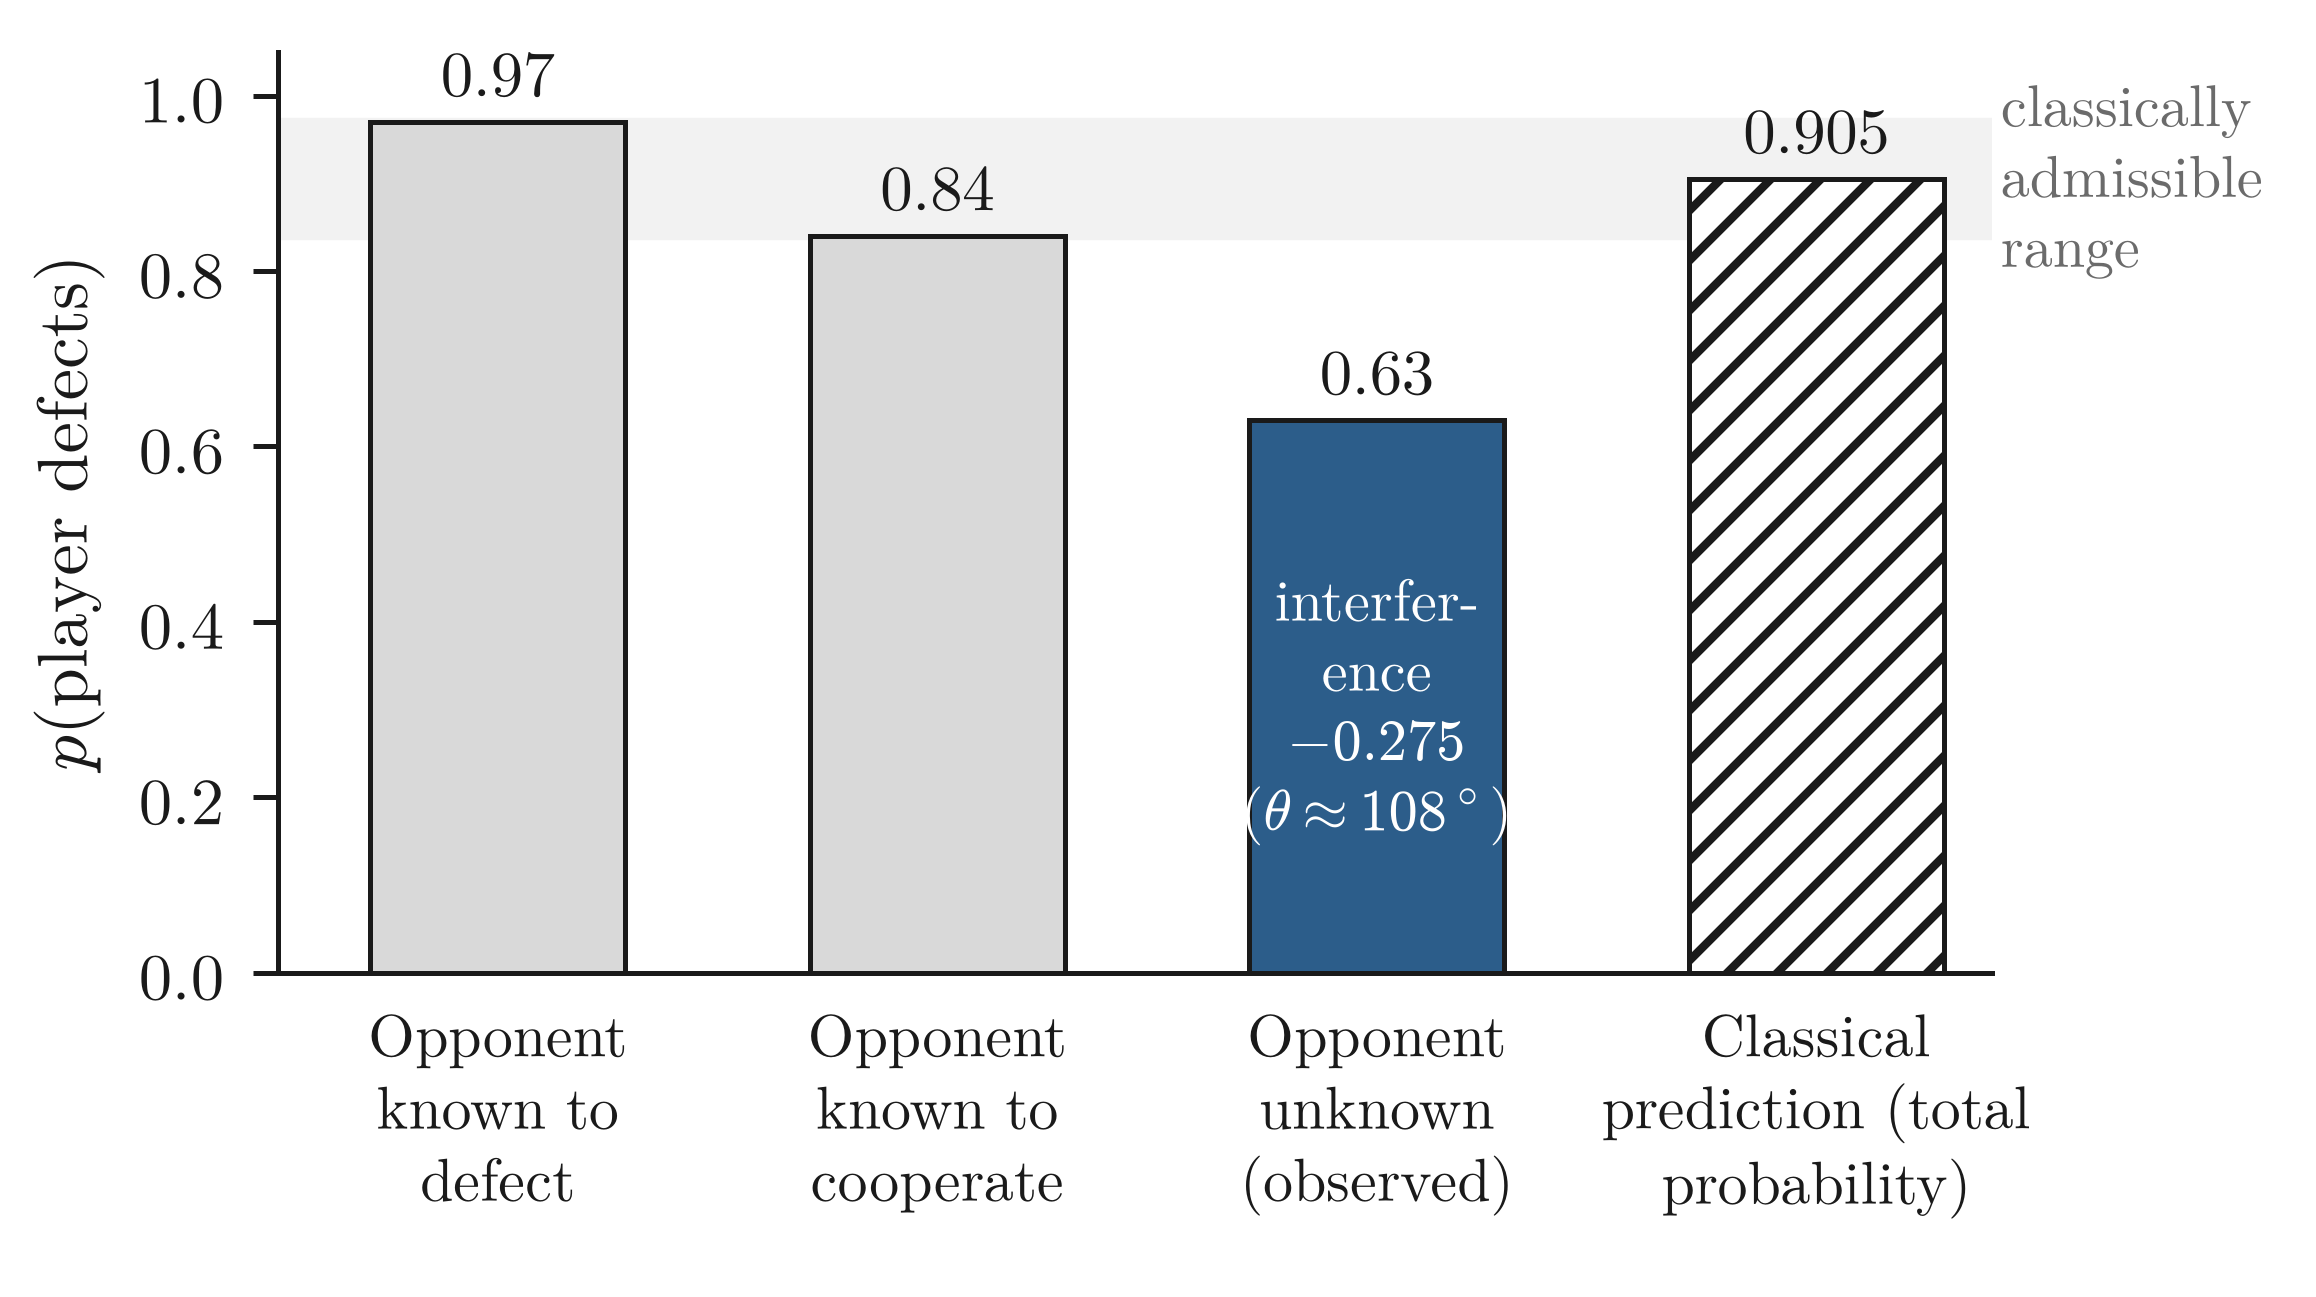
\includegraphics[width=0.75\textwidth]{figures/Fig4_interference.png}
\caption{Interference in the Prisoner's Dilemma disjunction effect. Observed defection rates from Shafir and Tversky (1992) and the classical prediction from the law of total probability with equal priors. The observed rate for the unknown condition lies outside the classically admissible range; QP accommodates it with an interference term of $-0.275$ (phase $\approx 108$\textdegree{}). Values computed with the code in Online Resource 2}\label{fig:interference}
\end{figure}

\subsection{Evidence: Where Quantum Models Outperform Classical Approaches, and Where They Do Not}\label{sec:evidence}
The strongest evidence comes from three kinds of test. The first is a priori, parameter-free predictions confirmed in new data, above all the QQ equality~\citep{Wang2014}. The second is dynamic signatures that Markov models cannot produce: interference of an intermediate choice on later confidence~\citep{Kvam2015}, oscillations in preference strength~\citep{Kvam2021} and a Zeno-like slowing of belief change under frequent measurement~\citep{Yearsley2016b}. The third is quantitative model comparison, where Hilbert-space multidimensional models compared favourably with Bayesian networks~\citep{Busemeyer2018} and a quantum sequential sampler compared favourably with the Bayesian sampler~\citep{Huang2025a}. Contextuality analyses that control for direct influences have also found genuine contextuality in carefully designed tasks~\citep{Cervantes2018,Basieva2019}, and a temporal Bell inequality was violated in one of the tested cases~\citep{Waddup2023}.

The picture is not one-sided. When the contextuality-by-default method was applied to earlier datasets, it found no true contextuality once direct influences were accounted for~\citep{Dzhafarov2016b}. In dynamic belief-change data, quantum advantages were confined to low-coherence conditions and shrank against a stronger Markov baseline~\citep{Busemeyer2019}. An open-system model of choice and response time was needed for only a subset of participants, the rest being fitted adequately by a Markov model~\citep{Epping2023}. Of the 71 theory and evidence studies in our corpus, 37 test their models on human data (E3) and 31 are formal models without data (Table \ref{tab:levels} and Online Resource 1). The fair summary is therefore that QP models outperform standard classical models on a well-defined class of phenomena involving incompatible, sequential or context-dependent judgements, and are unnecessary elsewhere. This class is exactly the one autonomous agents encounter when they interact with people.


%% -----------------------------------------------------------------------------
\section{Tier 1 (Deep) --- Perception, Memory and Decision-Making in Autonomous Systems}\label{sec:framework}
Sections \ref{sec:framework}--\ref{sec:multi} are organised in three tiers of depth: Tier 1 (this section) treats the functions with the most developed models, Tier 2 (Section \ref{sec:tier2}) the functions with partial evidence, and Tier 3 (Section \ref{sec:multi}) the speculative multi-agent applications. Figure \ref{fig:framework} maps the QP principles of Section \ref{sec:theory} onto these agent functions. Three questions recur: whether the judgements involved are incompatible (so that a single joint distribution does not exist), whether the agent's task requires predicting or aligning with such judgements, and whether the QP model makes an a priori prediction that could fail. Only when all three hold is a QP module likely to add value over a classical model; Section \ref{sec:compare} turns this into a decision guide.

\begin{figure}[ht]
\centering
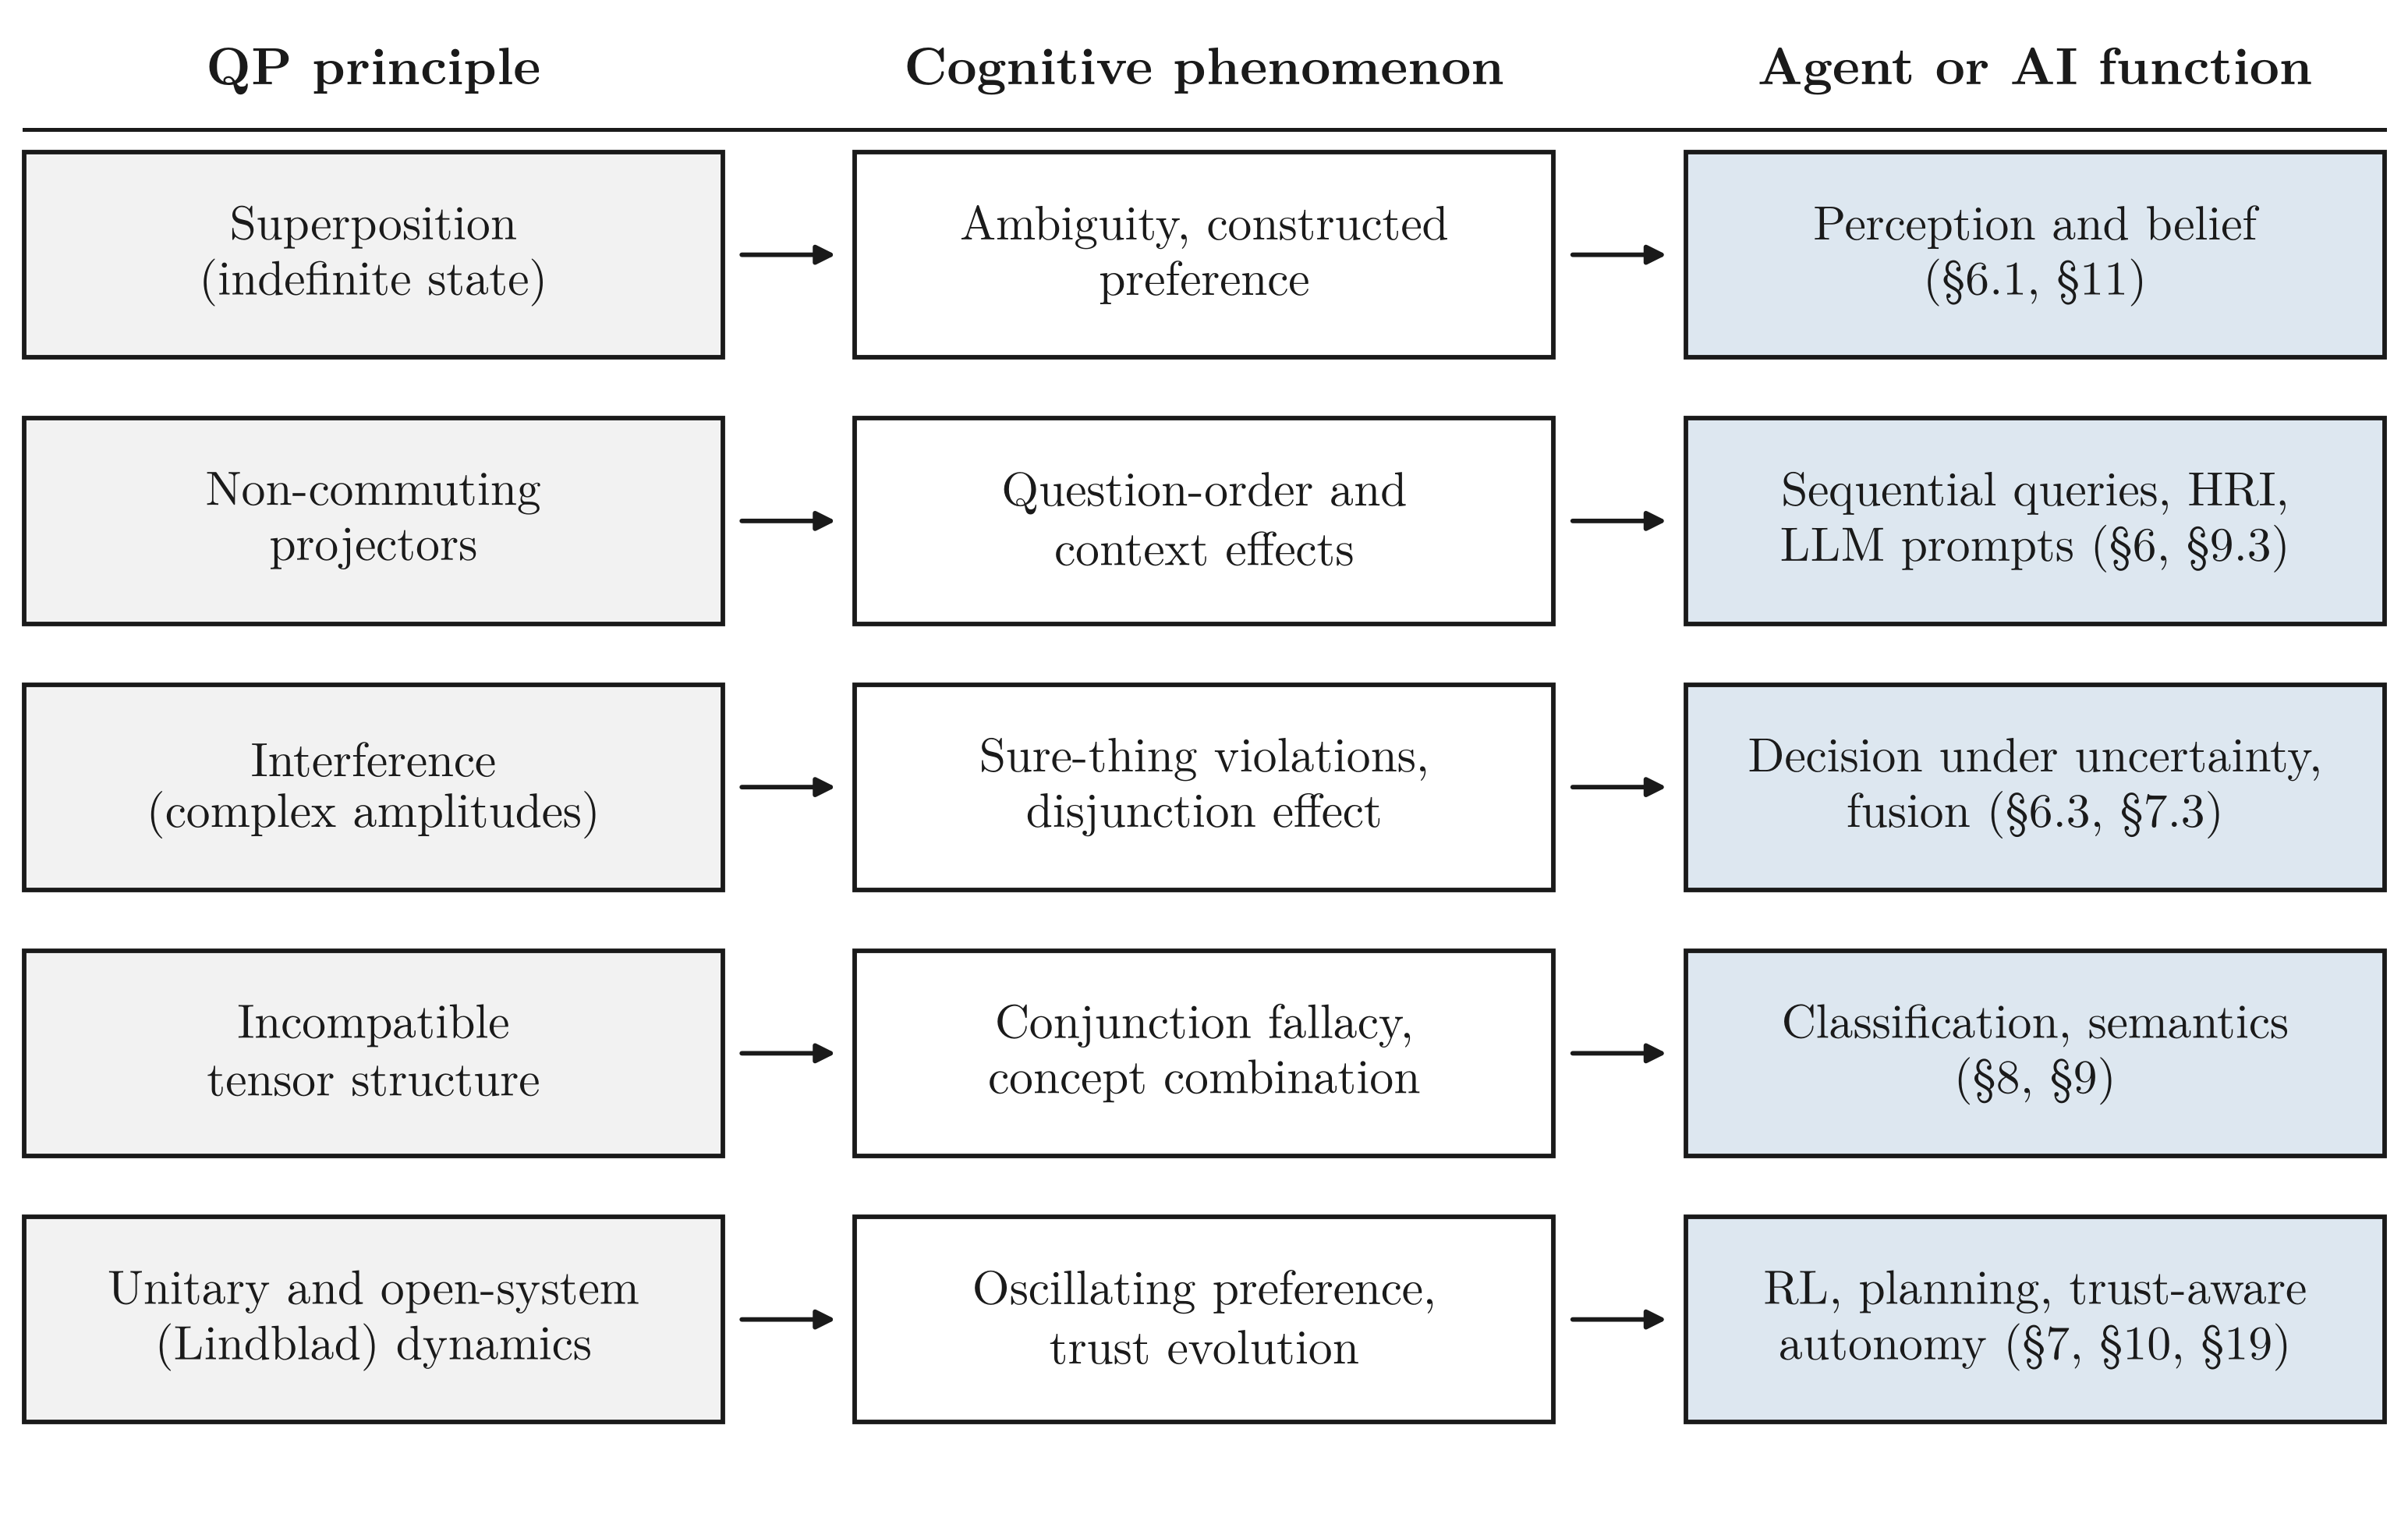
\includegraphics[width=1.00\textwidth]{figures/Fig5_framework.png}
\caption{From quantum-probability principles to cognitive phenomena and to the agent functions reviewed in this survey}\label{fig:framework}
\end{figure}

\subsection{Perception Under Sensor and Feature Ambiguity}\label{sec:ambig}

\subsubsection{Problem: Non-Independent Sensor and Feature Measurements}
Classical perception pipelines assume that each percept can be assigned a probability within one joint distribution over features. This assumption fails when features are not jointly measurable. Examples include ambiguous figures, vague categories whose boundaries shift with context~\citep{Blutner2013}, similarity judgements that are asymmetric and order-dependent~\citep{Pothos2013b}, and robots whose limited sensors cannot resolve mutually exclusive interpretations. In these cases the order in which features are queried, or the framing of the query, changes the outcome.

The problem has a second, human-facing side. Perception in human--robot teams is often shared: an operator reports what they see, confirms a robot's classification or is asked for a confidence rating. Human evidence accumulation does not behave like a classical random walk in such settings. When participants in a random-dot motion task had to make an explicit choice before rating their confidence, their later confidence differed from that of participants who rated without choosing, an interference effect that a quantum random-walk model fitted better than Markov models~\citep{Kvam2015}. Asking an operator to commit to a percept therefore changes the percept that the robot will later receive, which a fusion pipeline that treats human reports as independent measurements cannot represent.

\subsubsection{Quantum Solution: Entanglement and Superposition in Feature Spaces}
Lanza, Solinas and Mastrogiovanni proposed the first explicitly quantum-like robot perception model~\citep{Lanza2020}. A stationary robot with a front and a back presence sensor observes a moving object; the relative frequency of back-sensor events is encoded by a rotation into a single qubit, so that the qubit holds the balance between two mutually exclusive percepts and repeated measurement recovers their probabilities. The circuit reproduced the designed behaviour in simulation, whereas runs on real quantum processors showed large errors, particularly for unbalanced probabilities, and the authors recommend quantum-like simulation over current hardware. The multi-sensory extension encodes $n$ normalised sensor readings in $n$ qubits, so that the register holds a superposition over $2^n$ world configurations, and defines ``query operators'' that let the robot read out its degree of belief in a target configuration~\citep{Lanza2021}. Both studies are formal proofs of concept (E2): binary or colour percepts, no physical robot, a state destroyed by each query and no comparison with Bayesian or fuzzy fusion. They demonstrate representability, not improved perception.

The most recent robot study moves from representation to action. Chella et al.\ map a robot's sensor vector into a quantum feature space in which learned concepts or rule-defined perceptual regions are stored as reference states, and select reactive actions by their similarity to these references~\citep{Chella2026}. Two implementations, a quantum-kernel classifier compared with a classical radial-basis-function kernel and an illustrative circuit that selects actions by measurement after amplitude amplification, were evaluated offline on a public wall-following robot dataset, with errors concentrated near the boundaries between action regions. The authors present this explicitly as an offline proxy for reactive control rather than a closed-loop controller or evidence of quantum advantage, and its circuits use quantum computation, so it sits at the edge of this review's scope (E4).

Cognitive science supplies the templates that such robot models could follow but do not yet use. The quantum geometric model of similarity represents concepts as subspaces and computes similarity from sequential projections, so that asymmetries in similarity judgements emerge as order effects and violations of the triangle inequality as context effects~\citep{Pothos2013b}. Quantum-like concept representations account for the over- and under-extension of membership in combined concepts, such as ``pet fish'', that classical fuzzy-set models cannot fit~\citep{Aerts2009,Aerts2013}. Quantum-like Bayesian networks provide an inference engine that could combine such percepts with prior knowledge (Section \ref{sec:fusion})~\citep{Moreira2014}. For an autonomous agent, three uses follow. A QP percept can hold incompatible interpretations without forcing an early commitment; a QP model of a human observer can predict how that observer's reports depend on the order and framing of the robot's questions; and the order of perceptual queries becomes a design variable with a predictable effect. None of these uses has been tested on a robot.

\subsection{Memory and Episode Recognition}\label{sec:memory}

\subsubsection{Problem: Context-Dependent Retrieval and Associations}
Human memory is reconstructive: whether an item is recognised depends on the retrieval cue and on earlier retrievals, and people can simultaneously endorse mutually exclusive memory claims. Two signatures are well documented. In over-distribution, the probabilities of accepting an item as having appeared in each of two mutually exclusive conditions sum to more than the probability of accepting it as having appeared in either; in subadditivity, acceptance probabilities across exclusive and exhaustive instruction conditions sum to more than one~\citep{Trueblood2017b}. A classical memory store with fixed item probabilities cannot produce these patterns without additional mechanisms. Memory also interacts with judgement: people remember their own recent answers, and that record influences what they answer next, although a Bayesian observer would treat it as uninformative~\citep{Busemeyer2025}.

\subsubsection{Quantum Solution: Superposed Memory States and Contextual Collapse}
The generalised quantum episodic memory model treats verbatim and gist traces as incompatible features. Fitted to a new item-memory experiment and to published source-memory data, it accounts for subadditivity as well as over-distribution, which the dual-trace over-distribution model explains only in part~\citep{Trueblood2017b}. Busemeyer, Ozawa, Pothos and Tsuchiya compared three ways of incorporating episodic memory of one's own responses into quantum judgement models: an instrument-based account, a system-plus-environment account with an explicit recall operation, and a reformulation of the latter in instrument terms. The accounts differ in whether order effects arise from non-commuting projections or from belief updates, and in whether people must repeat an earlier answer when asked the same question again; the comparison is analytical, and the authors note that the empirical evidence on repeated questions is itself contested~\citep{Busemeyer2025}. Associative structure in the mental lexicon also has a quantum-like description~\citep{Bruza2009}, and order effects in the memory and belief queries of intelligent agents have been analysed in the same terms, with a maze example that contrasts classical and quantum decision scenarios~\citep{Kak2018}.

Three design implications follow for artificial agents. First, an agent that relies on human testimony, for example a service robot asking where an object was left or a decision aid eliciting an incident report, should expect recollections that endorse mutually exclusive claims and should not treat them as noise. Second, the order in which an agent queries a person's memory is a design variable, because each query changes the state that the next query probes. Third, the question of how an agent's record of its own past outputs should enter its next belief update, which is pressing for language-model agents that condition on their earlier answers, has a precise formulation in the instrument-based models. No robot or AI memory system based on these models has been reported, and their value for an artificial agent remains unestablished; their established value is in anticipating human recall.

\subsection{High-Stakes Decision-Making Under Uncertainty}\label{sec:decision}

\subsubsection{Problem: Violation of the Independence Axiom in Decisions}\label{sec:independence}
Expected-utility theory and the POMDP formalism rest on Savage's sure-thing principle~\citep{Savage1954}. Humans violate it (Section \ref{sec:interference})~\citep{Shafir1992}, and the Ellsberg paradox shows that ambiguity, not just risk, shapes choice~\citep{Ellsberg1961}. When an autonomous system must predict or collaborate with human decisions (in driving, triage, defence or shared control), a normative model will mispredict precisely those choices. The violations also arise from the decision process itself: asking a person to classify a situation before acting changes the action they take~\citep{Wang2016}, which matters for every interface in which a robot asks its operator to confirm a category first.

\subsubsection{Quantum Solution: Interference Effects in Sequential Decisions}
Quantum decision models represent the unresolved state of the world as a superposition, so that deciding with the uncertainty unresolved differs from deciding in each resolved case~\citep{Pothos2009,Busemeyer2012}. Quantum decision theory treats prospects as superpositions and splits a choice probability into a utility factor and an attraction (interference) factor, whose magnitude a ``quarter law'' fixes at about $0.25$ before any data are seen~\citep{Yukalov2011,Yukalov2016}. In the Prisoner's Dilemma data used to illustrate it, cooperation and defection probabilities with the partner's move unknown were 0.37 and 0.63, and the parameter-free prediction was 0.35 and 0.65~\citep{Yukalov2016}; the illustration rests on a single example. Its evolutionary extension addresses time-inconsistent choices~\citep{Yukalov2020}, and a quantum-conceptual account of expected-utility violations has been proposed~\citep{Aerts2011c}.

Interference also arises from an intermediate step. In three experiments with 721 participants, people who categorised a face before deciding how to act chose differently from the total probability implied by their categorisations, and a belief--action entanglement model predicted the pattern; the effect appeared in some conditions only~\citep{Wang2016}. An intermediate choice affects later confidence in the same way~\citep{Kvam2015}. Both results bear directly on agents that must first classify a situation (friend or foe, safe or unsafe) and then act, or that ask a human to do so. For prediction at scale, quantum-like Bayesian networks embed these effects in graphical models and set their interference phases by heuristics or by parameter-free laws rather than by fitting~\citep{Moreira2016,Wichert2020}; so far they have been evaluated on aggregate data from a few classic paradigms (Section \ref{sec:fusion}).

The most direct robotics application is Song et al.'s quantum-like Bayesian model of pedestrian crossing decisions for automated driving: the model captures crossings that a classical model treats as irrational and covers edge events in interactive scenes better than a Social-LSTM baseline~\citep{Song2022}. That study is a simulation on trajectory data (E4), and its interference parameters appear to be set rather than learned. It nonetheless marks the point at which quantum cognition entered a safety-critical autonomy problem. Quantum models of trust extend the same logic to decisions about relying on automation, with the strongest human-data support in the field (Section \ref{sec:map})~\citep{Roeder2023}.

\paragraph{Tier 1 at a glance} Table \ref{tab:tier1} summarises the three functions. In each, the cognitive models are tested on human data (E3), while the agent studies are formal models or offline simulations (E2--E4). The gap common to all three is the same: no study has placed a QP perception, memory or decision module in a closed loop with a robot and compared it with a classical module on the same task.

\begin{table}[ht]
\centering
\caption{Tier 1 functions: the QP models available, their strongest evidence, the agent studies and the main gap}\label{tab:tier1}
\footnotesize
\begin{tabular}{@{}>{\raggedright\arraybackslash}p{0.110\dimexpr\textwidth-10\tabcolsep\relax}>{\raggedright\arraybackslash}p{0.260\dimexpr\textwidth-10\tabcolsep\relax}>{\raggedright\arraybackslash}p{0.230\dimexpr\textwidth-10\tabcolsep\relax}>{\raggedright\arraybackslash}p{0.190\dimexpr\textwidth-10\tabcolsep\relax}>{\raggedright\arraybackslash}p{0.210\dimexpr\textwidth-10\tabcolsep\relax}@{}}
\toprule
\textbf{Function} & \textbf{QP models} & \textbf{Strongest evidence} & \textbf{Agent studies} & \textbf{Main gap} \\
\midrule
Perception & Qubit percepts~\citep{Lanza2020,Lanza2021}; quantum similarity~\citep{Pothos2013b}; quantum walk of evidence~\citep{Kvam2015} & Interference of an intermediate choice on confidence (E3)~\citep{Kvam2015} & \citet{Lanza2020,Lanza2021} (E2); \citet{Chella2026} (E4, offline) & No comparison with Bayesian or fuzzy fusion; no closed loop \\
Memory & Generalised quantum episodic memory~\citep{Trueblood2017b}; instruments with memory~\citep{Busemeyer2025} & Over-distribution and subadditivity fitted (E3)~\citep{Trueblood2017b} & \citet{Kak2018} (E2, conceptual) & No artificial-agent memory built on these models \\
Decision & QP decision models~\citep{Pothos2009}; quantum decision theory~\citep{Yukalov2011}; QLBNs~\citep{Moreira2016}; belief--action entanglement~\citep{Wang2016} & Disjunction effect and categorisation interference (E3)~\citep{Pothos2009,Wang2016} & \citet{Song2022} (E4) & Interference parameters set, not learned; no closed-loop test \\
\bottomrule
\end{tabular}
\end{table}


%% -----------------------------------------------------------------------------
\section{Tier 2 (Medium) --- Learning, Planning and Sensor Fusion}\label{sec:tier2}

\subsection{Quantum Reinforcement Learning in Autonomous Agents}\label{sec:qirl}

\subsubsection{Exploration vs. Exploitation Trade-off}
Every RL agent must balance exploiting what it knows against exploring what it does not. Classical agents use $\varepsilon$-greedy, softmax or optimism-based rules~\citep{Sutton2018}. Quantum-inspired RL replaces these with a representation in which each state holds a superposition of actions and action selection is a measurement.

\subsubsection{Quantum Superposition for Policy Search and Value Functions}
Dong, Chen, Li and Tarn's quantum RL (QRL) stores, for each state, amplitudes over ``eigen-actions''; rewards drive Grover-style amplitude amplification of the chosen action, so the exploration probability adapts automatically~\citep{Dong2008}. The robust quantum-inspired variant was validated on a real mobile robot and was more robust to the learning rate than temporal-difference learning~\citep{Dong2012}, and quantum-inspired experience replay extends the idea to deep RL~\citep{Wei2022}. These algorithms are classical and should be judged against modern classical exploration strategies. Our illustrative experiment in Section \ref{sec:rl-exp} does exactly this and finds a clear trade-off: faster early learning with noisy rewards, but no stable convergence. Projective simulation is a different, physics-motivated agent model in which deliberation is a random walk through episodic memory~\citep{Briegel2012}. Its convergence in Markov decision processes has been proved~\citep{Boyajian2020}, a photonic hardware architecture has been proposed for it~\citep{Flamini2020}, a photonic experiment demonstrated a quantum speed-up in learning~\citep{Saggio2021}, and its classical version has been benchmarked against Q-learning and SARSA~\citep{Melnikov2018} and used on real robots (Section \ref{sec:affordance}). Variational-circuit RL, which uses quantum computation rather than QP as a model of cognition, is reviewed in the companion survey (Section \ref{sec:vqcrl}).

\subsection{Planning Under Uncertainty}\label{sec:planning}

\subsubsection{Classical Planners and State Representation Limitations}
Classical planners and POMDP solvers represent belief as a distribution over a fixed state space~\citep{Lauri2023}. They cannot represent the context-dependent preferences and goals of human partners, which may be constructed during interaction rather than retrieved~\citep{Kvam2021}.

\subsubsection{Quantum Planning: Superposed Goal States and Interference in Paths}
Two different ideas are at work. Quantum algorithms that search plan spaces faster belong to quantum computing and are reviewed in the companion survey~\citep{Guru2026}; they inherit the limits of noisy hardware~\citep{Preskill2018}. The cognitive idea uses quantum dynamics to model deliberation. Quantum walks over option networks can produce choice probabilities that violate the sure-thing principle~\citep{MartinezMartinez2016}, Lindblad models describe how a deliberating agent escapes classical equilibria~\citep{Asano2026}, and a maze example contrasts classical and quantum decision scenarios for an intelligent agent~\citep{Kak2018}. Such models could let a planner anticipate how a human collaborator's goals will shift, but none has yet been integrated into a robot planner. We found no evidence that QP planning improves plan quality for autonomous systems, and we regard this as an open research question rather than an established capability.

\subsection{Multi-Source Fusion with Non-Independent Modalities}\label{sec:fusion}

\subsubsection{Problem: Kalman Filter and Classical Fusion Assumptions Break Down}
The Kalman filter is optimal for linear-Gaussian systems with known noise~\citep{Kalman1960}, and its non-linear and learned variants dominate robotic state estimation~\citep{Haykin2001,Thrun2005}. Its assumptions (a single joint distribution, independent noise, order-invariant updates) are appropriate for physical sensors measuring the same physical quantity. They break down when ``sensors'' are judgements from different contexts, for example a human report, a language instruction and a vision classifier, whose outputs cannot be embedded in one joint distribution. It is important to be precise here: for physical pose estimation from independent Gaussian sensors, QP adds nothing and the Kalman filter remains optimal (Section \ref{sec:case-fusion}).

\subsubsection{Quantum Fusion: Entangled State Updates and Measurement Context}
Quantum-like Bayesian networks (QLBNs) replace the conditional probabilities of a Bayesian network with complex amplitudes, so marginalising over an unobserved node produces interference terms~\citep{Moreira2014,Moreira2016}. The central difficulty is that every unobserved node adds a free phase. Successive work has proposed heuristics, including a similarity heuristic~\citep{Moreira2016}, a ``law of balance'' and ``law of maximum uncertainty''~\citep{Wichert2020} and influence diagrams that add utilities~\citep{Moreira2020b}, to set the phases without fitting them to the data being predicted. Extensions combine QLBNs with belief entropy for multi-attribute decisions~\citep{She2021}, with Dempster--Shafer evidence theory~\citep{Gao2025}, and with entanglement to capture biased selection, where a biased entangled model achieved an RMSE of 3.4 on Prisoner's Dilemma data, the best among the models compared~\citep{Meghdadi2022}. In multimodal ML, quantum-inspired fusion treats each modality's decision as a measurement in an incompatible basis; on video sentiment benchmarks this outperformed decision-level and content-level fusion and handled cases in which every unimodal classifier failed~\citep{Gkoumas2021,Li2021a}. These results are on benchmark labels, not human decision data, and the incompatibility assumption itself was not tested.


%% =============================================================================
\surveypart{Part C --- Applications and Validation (Sections 8--16)}

\section{Quantum Cognition for Machine Learning and AI}\label{sec:ml}

\subsection{Feature Learning and Representation Problem}\label{sec:features}

\subsubsection{Classical Approach: Dimensionality Reduction (PCA, t-SNE)}
Classical representation learning maps inputs to real-valued feature vectors, whether by linear projections such as PCA, non-linear embeddings such as t-SNE, or learned deep features~\citep{Krizhevsky2012}. Probabilities are then obtained by a fixed read-out (for example softmax), which produces a single joint distribution over labels regardless of the order or context of the query.

\subsubsection{Quantum Approach: Superposed Feature Spaces and Entangled Representations}
Three distinct ideas appear in the literature and should not be conflated. Quantum kernel methods map data into a quantum feature Hilbert space and require quantum hardware for any advantage~\citep{Schuld2019,Biamonte2017}. Their advantages are fragile, because trainability limits~\citep{Cerezo2021} and dequantisation results~\citep{Tang2019,Aaronson2015} often remove the claimed speed-up. Quantum-inspired representations use complex-valued vectors and density matrices on classical hardware: a word is a superposition of semantic ``sememes'', a sentence is a mixture, and matching is a measurement~\citep{Li2019,Zhang2018,Zhang2025}. Finally, quantum-cognitive representations aim to reproduce human-like judgement patterns rather than to improve accuracy~\citep{Maksimovic2025}. Tensor-network classifiers, which are classically simulable quantum-style models, reached below 1\% test error on MNIST~\citep{Stoudenmire2016}. Quantum-inspired matching models have typically performed comparably to strong CNN and RNN baselines rather than better, while offering representations their authors describe as more interpretable~\citep{Li2019}. Those interpretability claims have not been tested with users.

\subsection{Classification Under Label Ambiguity}\label{sec:labels}

\subsubsection{When Multiple Labels Apply Simultaneously: Order-Dependent Classification}
Real categories are vague and overlapping, and human annotators' labels depend on which category is considered first~\citep{Blutner2013,Wang2016}. A softmax classifier assigns a single distribution over labels and cannot represent the fact that the answer to ``is it a cat?'' depends on whether ``is it wild?'' was asked first. For ML systems trained on human labels, or used alongside human decision-makers, this is a modelling mismatch rather than label noise.

\subsubsection{Quantum Cognition: Interference in Multi-Class Decisions}
Representing labels as non-commuting projectors on a learned state produces order-dependent label judgements (Case Study 2, Section \ref{sec:case-label}). Quantum-cognitively motivated decision fusion used this structure to combine modality-specific sentiment judgements~\citep{Gkoumas2021}, and a survey of quantum-cognitively inspired sentiment analysis maps the design space~\citep{Liu2023}. Quantum-cognitive neural networks that use tunnelling-inspired activations reproduced human-like confidence and uncertainty on image classification and trained up to 50 times faster than their classical counterpart. That human-likeness was assessed by simulation rather than against participant data~\citep{Maksimovic2025}. No study has yet shown that order-aware QP classifiers improve agreement with individual human annotators on a standard benchmark; this is a clear, testable gap (Benchmark 3, Section \ref{sec:bench}).

\subsection{Knowledge Representation and Semantic Similarities}\label{sec:semantics}
Quantum logic has a long history in semantic representation. Widdows and Peters showed that negation and disjunction on word vectors behave as quantum-logical connectives, allowing unwanted word senses to be removed from queries~\citep{Widdows2003}. Density-matrix language models captured term dependencies for retrieval~\citep{Sordoni2013}, and a survey of quantum-theory-inspired information retrieval covers representation, ranking and user cognition~\citep{Uprety2021}. Widdows, Kitto and Cohen give the broadest account of quantum mathematics in AI~\citep{Widdows2021}. Compositional quantum NLP (DisCoCat) was run on real quantum hardware for small sentence-classification tasks, a feasibility demonstration with small datasets, long queue times and no quantum advantage~\citep{Lorenz2023}; two reviews cover the field~\citep{Widdows2024,Nausheen2025}. Contextual word embeddings have been recast in terms of quantum contextuality, as a framework without an empirical evaluation~\citep{Svozil2025}. For agents, such as robots grounding language instructions or dialogue systems tracking context, the relevant contribution is a principled way to represent meaning that depends on context. The contribution does not come from quantum computation.


%% -----------------------------------------------------------------------------
\section{Quantum Cognition for Deep Learning}\label{sec:dl}

\subsection{Activation and Representation Learning}

\subsubsection{Classical DL: Neuron Activations as Probabilities}
In standard deep networks, activations are real numbers and output probabilities come from a softmax. Uncertainty is typically estimated post hoc (ensembles, dropout, Bayesian layers), and all outputs are assumed to live in one classical probability space.

\subsubsection{Quantum DL: Superposed Activations and Non-Classical Interference}
Complex-valued, quantum-inspired networks carry phases as well as magnitudes, so that intermediate representations can interfere. CNM encodes words as complex superpositions and sentences as density matrices and matched strong baselines on question answering~\citep{Li2019}. A quantum many-body wave-function view of language modelling offered a theoretical justification for CNN structure~\citep{Zhang2018}, and a recent sequence model with unitary Hamiltonian dynamics and Born-rule decoding proves an expressivity gain on a constructed task family but has not yet been tested on language data~\citep{Nebli2026}. Quantum-inspired networks for conversational emotion recognition~\citep{Li2021b} and multimodal sentiment~\citep{Li2021a} performed on a par with the state of the art. Quantum Bayesian neural networks propose quantum algorithms for posterior sampling but were evaluated only in classical simulation~\citep{Berner2021}. The consistent pattern is parity, not superiority, on accuracy, with claims of interpretability that remain to be tested.

\subsection{Backpropagation and Gradient Descent Under Uncertainty}

\subsubsection{Problem: Gradient Vanishing and Loss-Function Plateaus}
Deep networks face vanishing gradients; variational quantum circuits face the more severe problem of barren plateaus, in which gradients vanish exponentially with the number of qubits for global cost functions~\citep{Cerezo2021}. This is a limitation of quantum hardware models, not of quantum-like models run classically, which are trained with ordinary automatic differentiation~\citep{Bergholm2018,Broughton2020}.

\subsubsection{Quantum Gradient Descent: Do Superposed Weight Updates Help?}
We found no evidence that ``superposed weight updates'' improve the training of classical deep networks, and we caution against the claim. Where quantum circuits are trained, gradients are estimated by parameter-shift rules and inherit barren-plateau and noise limits~\citep{Cerezo2021,Preskill2018}. Where quantum-inspired networks are trained classically, their complex-valued parameters are optimised by standard gradient descent. The contribution of quantum cognition to optimisation is therefore conceptual, for example modelling how a learner's uncertainty about incompatible hypotheses evolves, rather than algorithmic.

\subsection{Attention Mechanisms and Multi-Head Architectures}\label{sec:llm}

\subsubsection{Order-Dependent Attention: Measurement Sequence in Transformer Models}
Transformer outputs depend on prompt order and framing. Human-like response biases in survey-style prompts were found only partially, and inconsistently, across nine LLMs~\citep{Tjuatja2024}, while cognitive-psychology batteries revealed both human-like and non-human-like reasoning in GPT-3~\citep{Binz2023}. Quantum-cognition methods give these observations a precise vocabulary and test statistics. Lo, Sadrzadeh and Mansfield constructed a linguistic schema modelled on a contextual quantum scenario and, using a masked language model, found about 0.15\% of instances contextual under the sheaf-theoretic criterion and about 71\% under contextuality-by-default~\citep{Lo2025}. Context effects in LLM similarity judgements mirror human order effects in some settings but not others~\citep{Uprety2024}. Bell-type tests on LLM concept combinations reported violations and Bose--Einstein-like word statistics resembling human data~\citep{Aerts2026}. GPT-5 committed far fewer conjunction fallacies than humans, and its judgement pattern was closer to early QP models than to the noisy variants that fit people~\citep{Imannezhad2026}. An audit of question-order effects with the QQ equality found near-deterministic saturation in a small model, showing that the QQ test can be uninformative when an LLM's answers are saturated~\citep{Kang2026}. Together these studies suggest that attention-based models exhibit some context effects that QP models describe well, but they do not show that transformers are quantum-like in general. The analogy between attention and ``soft measurement'' remains a hypothesis to be tested (Section \ref{sec:vs-attention}).


%% -----------------------------------------------------------------------------
\section{Quantum Cognition for Reinforcement Learning}\label{sec:rl}

\subsection{Markov Decision Process (MDP) Assumptions and Their Violations}\label{sec:mdp}

\subsubsection{Problem: Memory Dependencies and Context Effects}
RL assumes the Markov property and stationary, additive rewards~\citep{Sutton2018}. Human feedback, which increasingly shapes RL for robots and LLMs, violates both: evaluations depend on what was asked before, preferences oscillate over time~\citep{Kvam2021}, and trust evolves non-monotonically~\citep{Roeder2023}. Reproducibility studies also show how sensitive deep RL is to seeds and hyperparameters, which sets a high bar for claims of improvement~\citep{Henderson2018}.

\subsubsection{Quantum RL: Non-Markovian Memory and State Superposition}
Open-system quantum--Markov models provide a principled way to model non-Markovian, context-dependent reward sources~\citep{Busemeyer2020,Epping2023}. They combine Markov and quantum dynamics in one Lindblad equation, with a single weight that sets the balance between the two, so that classical random-walk behaviour is a special case rather than a competitor~\citep{Busemeyer2020}. Their empirical motivation is directly relevant to human feedback. Preference strength oscillates systematically over time, and eliciting a choice early changes the later oscillation~\citep{Kvam2021}; in a pairwise-choice task the pure Markov model sufficed for most participants, but a substantial minority required the open-system model~\citep{Epping2023}; and in sequential inference the order in which evidence is presented changes the final judgement in a way that a QP model reproduces and an anchoring-and-adjustment model does not~\citep{Trueblood2011}.

For RL from human feedback, this suggests three concrete uses. A QP model of the evaluator can predict how a person's comparison of two trajectories depends on what they were shown before; it can be used to choose the order in which comparisons are presented so that the collected preferences are less order-biased; and its Markov--quantum weight separates genuine changes of preference from random variation. To our knowledge no RL algorithm has yet used such a model of the human reward-giver, which we identify as a promising direction (Section \ref{sec:directions}). The test is simple to state: fit the open-system model and a Markov model to counterbalanced human comparisons, and train the same agent on rewards corrected by each.

\subsection{Policy Search and Exploration Strategies}\label{sec:vqcrl}

\subsubsection{Classical RL: Epsilon-Greedy, Softmax, Boltzmann Exploration}
Classical exploration strategies are simple, well understood and hard to beat on small problems~\citep{Sutton2018}, and deep RL for real robots has succeeded mainly through careful engineering and simulation-to-real transfer rather than new exploration principles~\citep{Lauri2023}.

\subsubsection{Quantum RL: Quantum Superposition for Simultaneous Action Evaluation}
Three lines coexist, and only the first is in the scope of this review. Quantum-inspired RL (Section \ref{sec:qirl}) is classical: action amplitudes are ``measured'' to select an action, and amplitude amplification shifts the policy towards rewarded actions~\citep{Dong2008,Dong2012,Wei2022}. Quantum-agent theory proves speed-ups in deliberation and learning separations on specially constructed tasks~\citep{Dunjko2018}. Reinforcement learning with parametrised quantum circuits in place of neural networks uses quantum computation as a function approximator rather than QP as a model of cognition; it is reviewed, with its robot studies, in the companion survey~\citep{Guru2026} and in dedicated surveys~\citep{Meyer2022,Chen2024}. Its one consistent benefit there is parameter efficiency, and no study shows better policies than tuned classical networks of comparable compute. The question for this review is different: whether a QP model of how a learner, or a human teacher, holds and revises incompatible evaluations helps an agent learn. No study has yet tested this.

\subsection{Value Estimation and Q-Learning Under Uncertainty}\label{sec:value}

\subsubsection{Order Effects in Temporal-Difference Learning}
Temporal-difference learning is order-sensitive by construction: the same experiences presented in different orders yield different value estimates. Classical RL treats this as a nuisance that experience replay reduces. Quantum cognition suggests an alternative reading when the learner is human-like: order effects in the evaluation of evidence are systematic and predictable~\citep{Trueblood2011,Trueblood2017a}.

\subsubsection{Quantum Q-Values: Interference in Reward Prediction (Not Yet Demonstrated)}
Interference in reward prediction has not been demonstrated as a benefit in any benchmark we found. The quantum-inspired results that exist concern robustness rather than value accuracy: on a 58-state task and on a real mobile robot, quantum-inspired RL converged across a wider range of learning rates than temporal-difference learning~\citep{Dong2012}. In our own illustrative experiment (Case Study 3, Section \ref{sec:rl-exp}), amplitude-based exploration without a mechanism for reducing amplitudes became unstable under reward noise, which highlights a design gap rather than an advantage.

A fair test of interference in value estimation would hold three things fixed: the state representation, the number of environment interactions and the tuning budget of the classical baseline. It would then compare amplitude-based value updates that can both increase and decrease with tuned TD learning, on tasks whose rewards come from a context-dependent source such as human evaluations, because that is where QP structure is expected. Benchmark 4 (Section \ref{sec:bench}) sets out the tasks, baselines and metrics for it.


%% -----------------------------------------------------------------------------
\section{Quantum Cognition for Physical AI and Embodied Systems}\label{sec:robots}

\subsection{Sensorimotor Integration and Body Schema}\label{sec:embodied}

\subsubsection{Problem: Proprioception, Interoception and Multimodal Ambiguity}
Embodied agents must integrate signals whose meaning depends on the body's state and the task: proprioceptive, interoceptive, tactile and visual signals can conflict, and their interpretation depends on what the agent is trying to do. Predictive-processing accounts cast this as prediction-error minimisation over a generative model~\citep{Friston2010,Clark2013}. Classical cognitive architectures implement it with symbolic and probabilistic modules~\citep{Laird2017,Kotseruba2020}.

\subsubsection{Quantum Embodied Cognition: Entangled Sensor-Motor States}
Robot-facing proposals fall into four groups (Online Resource 1, Table S1). The first is quantum-like perception models, already discussed~\citep{Lanza2020,Lanza2021}. The second is quantum-circuit models of robot ``thinking'' and control: a classic--quantum dialogue model of robot creativity~\citep{Mannone2024}, a teleo-reactive robot whose action rules are evaluated by quantum kernels and measurement-based circuits, reaching about 0.91 accuracy offline on wall-following data~\citep{Chella2026}, and a neuro-cognitive agent architecture using Grover and Deutsch--Jozsa routines in a game environment~\citep{Daglarli2025}. The third is quantum models of robot emotion and affect: emotion spaces encoded in qubits~\citep{Yan2019}, Plutchik-based emotion circuits for companion robots~\citep{Yan2021c}, a review of emotion-space models~\citep{Yan2021b}, mixed states of reflection and affect realised as small entangling circuits~\citep{Hoorn2019}, the Q-Copp\'elia affective decision framework for human--robot interaction (HRI), which its authors present as a theoretical exercise because the circuit needs too many qubits even to simulate~\citep{Ho2022}, an early quantum-automata model of emotional robot behaviour~\citep{Lukac2007} and the QUADRI social-robotics programme~\citep{DeCarolis2025}. The fourth is architectural positions~\citep{Aerts2011d,Moreira2020a}. Of the 17 robot-facing studies, 11 are at E1--E2: circuits and formal models without user studies or classical baselines. The circuit-based models also blur the line between quantum-like modelling and quantum computing, which should be made explicit because only the former is deployable today. Figure \ref{fig:architecture} shows how a quantum-like module can sit in an embodied agent.

\begin{figure}[ht]
\centering
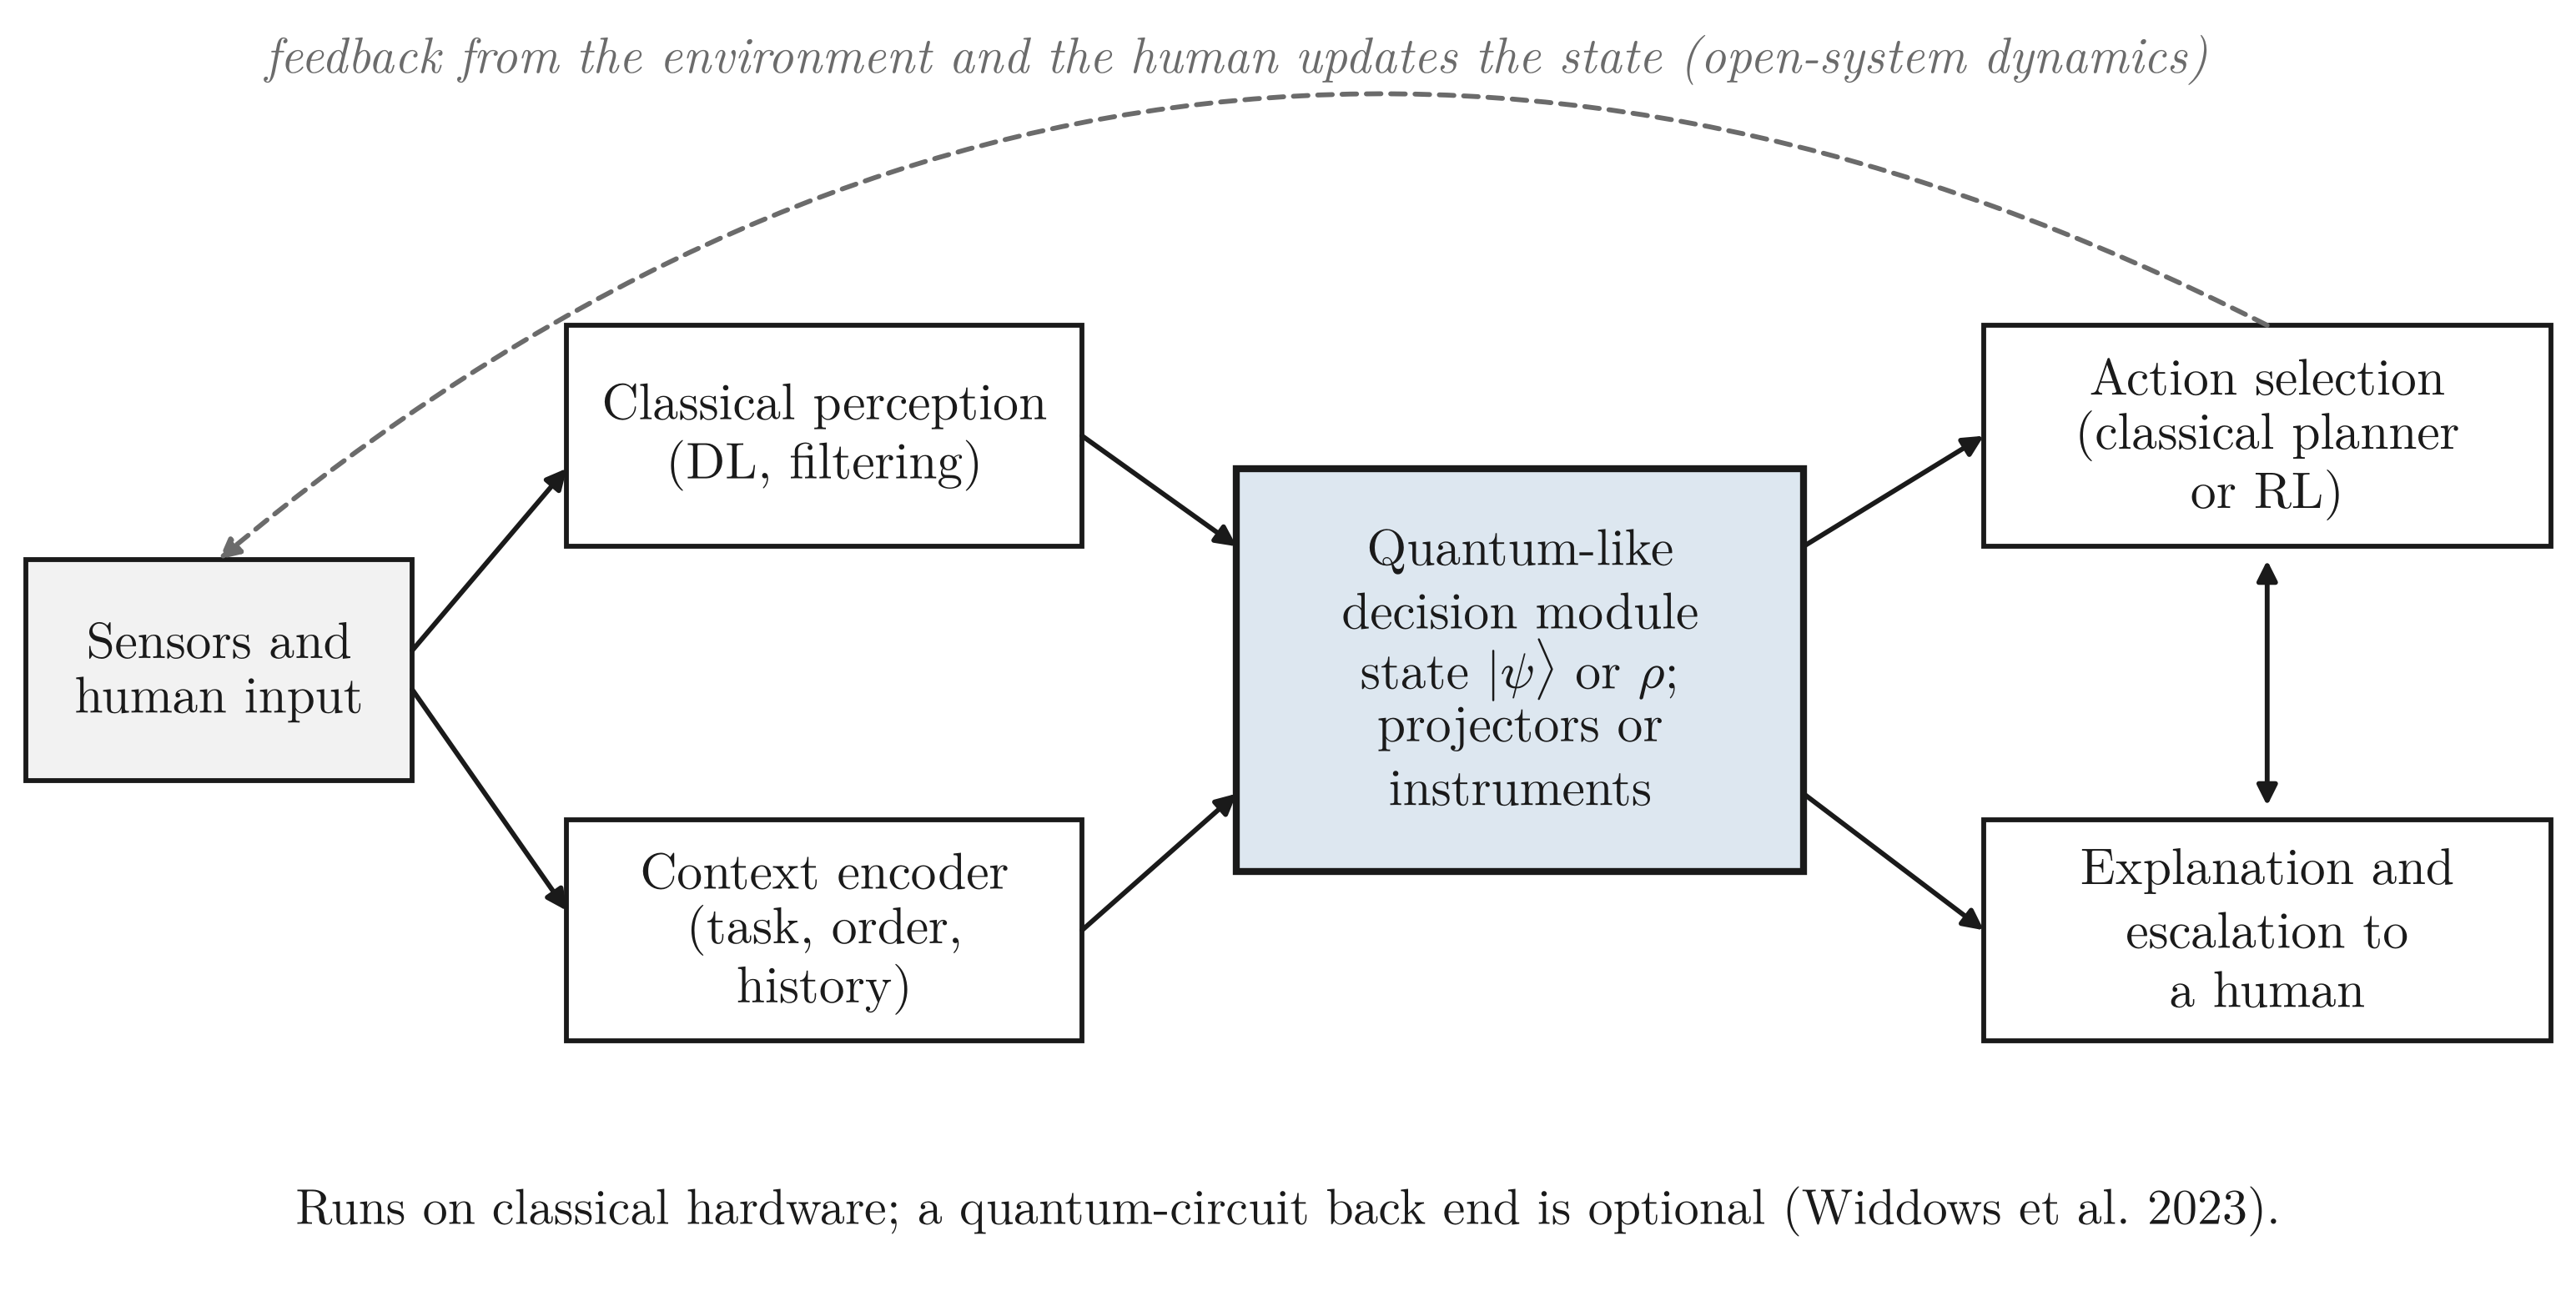
\includegraphics[width=1.00\textwidth]{figures/Fig6_architecture.png}
\caption{A hybrid architecture for a quantum-like decision module in an autonomous agent. Classical perception and a context encoder feed a QP state; context-dependent measurements (projectors or instruments) produce graded, order-aware judgements that a classical planner or RL policy acts on, with explanation and escalation to a human. Feedback updates the state as an open system}\label{fig:architecture}
\end{figure}

\subsection{Affordance Perception and Action Selection}\label{sec:affordance}

\subsubsection{Classical Approach: Discrete Action Sets and Binary Affordances}
Classical robots typically treat affordances (what an object allows the robot to do) as discrete, independently detectable properties, and select actions by maximising expected utility over a fixed action set.

\subsubsection{Quantum Approach: Superposed Affordances and Interference in Action Space}
The most mature embodied line is not quantum cognition but projective simulation (PS) run classically. A real robot learned hierarchical manipulation skills through play, reaching 90\% success in about 80 roll-outs in simulation~\citep{Hangl2016}, and PS with active learning and behaviour composition solved previously unsolvable tasks and improved learning speed by about 30\%~\citep{Hangl2020}. Superposed affordances in the QP sense, where an object's affordances are incompatible and the order of evaluation matters, have not been implemented on a robot. They remain a hypothesis (Section \ref{sec:multi-open}).

\subsection{Predictive Processing and Action Prediction Errors}\label{sec:predictive}

\subsubsection{Order-Dependent Prediction Errors in Physical Interaction}
Predictive processing treats perception and action as the minimisation of prediction error~\citep{Friston2010,Clark2013}. Quantum-like models add one ingredient: the order in which predictions are tested can change the result. In physical interaction, such as handover, shared manipulation or co-driving, the human partner's intentions are themselves constructed during the interaction~\citep{Kvam2021}, so a robot that queries (by gesture, speech or motion) changes what it is trying to predict. We know of no experiment that tests this in physical HRI; the handover setting often cited for it has no published quantum-like study, and the related works listed in some bibliographies could not be verified (Section \ref{sec:search}).


%% -----------------------------------------------------------------------------
\section{Tier 3 (Shallow) --- Speculation on Multi-Agent Coordination and Collective Cognition}\label{sec:multi}

\subsection{Quantum Cognition in Multi-Robot Coordination}\label{sec:teams}
Quantum game theory showed that entangled strategies can escape classical dilemmas~\citep{Eisert1999}. Physical entanglement between robots and quantum communication links belong to the companion survey~\citep{Guru2026}; quantum-like approaches instead model interdependent agents. Lawless argues that interdependence in autonomous human--machine teams is quantum-like: team performance is not decomposable into member contributions~\citep{Lawless2020,Lawless2023,Lawless2025}. Human interaction data show context sensitivity that a quantum model fitted better than a matched classical model~\citep{Waddup2021}. Quantum game models, simulated classically, have been proposed for interaction-aware automated driving with two players~\citep{Essalmi2025} and with several players and strategies, where they raised success rates and reduced collisions against classical game-theoretic models in simulation~\citep{Essalmi2026}; an independent reproduction of the earlier model could not confirm its collision results. Multi-robot emotion fusion through entangled qubit encodings remains a formal model~\citep{Yan2021a}.

\subsection{Distributed Quantum-Like Decisions Across Swarms}\label{sec:swarms}
Networks of quantum decision-makers exchanging information converge to consensus and reproduce a dynamic disjunction effect~\citep{Yukalov2018,Yukalov2022}, and affective AI has been framed as a ``quantum operation'' combining cognition and emotion~\citep{Yukalov2023}. Quantum stochastic walks give a network model of decision~\citep{MartinezMartinez2016}. PS swarms reproduce collective motion~\citep{Ried2019}, foraging-dependent alignment~\citep{LopezIncera2020} and queue formation with polarisation near 0.99~\citep{Kong2026}, all in simulation with classical PS.

\subsection{Concept Learning and Semantic Emergence}\label{sec:concepts}
Entangled concept combinations~\citep{Aerts2011a}, Fock-space concept dynamics~\citep{Aerts2013} and Bell-type structure in LLM language~\citep{Aerts2026} suggest that shared meaning in groups of agents could be modelled with quantum structure. Whether such models help artificial agents develop shared concepts is untested.

\subsection{Open Questions for Future Research}\label{sec:multi-open}
\begin{itemize}
\item Can a quantum-like model of human teammates improve a robot team's coordination with people, compared with Bayesian theory-of-mind models?
\item Do quantum-like consensus models predict human--robot group decisions better than classical opinion dynamics?
\item Are ``superposed affordances'' measurable in human behaviour during joint action, and do they help a robot anticipate its partner?
\item Which multi-agent claims survive when compared with classical models of equal parameter count, as the quantum game models of driving still need to be~\citep{Essalmi2025,Essalmi2026}?
\end{itemize}


%% -----------------------------------------------------------------------------
\section{Prior Work and Positioning}\label{sec:synthesis}
This section positions the primary literature and synthesises the evidence of Sections \ref{sec:theory}--\ref{sec:multi}; earlier \emph{reviews} are compared in Section \ref{sec:related}.

\subsection{Quantum Cognition in Psychology}
The psychological literature is mature, with a textbook~\citep{Busemeyer2012}, a BBS target article~\citep{Pothos2013a}, tutorials~\citep{Yearsley2016a,Yearsley2017}, reviews~\citep{Bruza2015,Pothos2022,Huang2025b} and an active critical literature (Sections \ref{sec:evidence} and \ref{sec:compare}). Its models are fitted to human data, which places 37 of the 71 theory and evidence studies at level E3.

\subsection{Quantum Probability in Decision Science and Cognitive Science}
Quantum decision theory~\citep{Yukalov2011,Yukalov2016}, contextual probability~\citep{Khrennikov2010,Khrennikov2023b}, contextuality-by-default~\citep{Dzhafarov2016a} and quantum-like heuristics~\citep{Huang2025c} provide alternative formalisms. A 2015 survey organised quantum-like decision models by formalism~\citep{Ashtiani2015}.

\subsection{Application to Robotics, AI, ML, DL and RL (2020--2026)}\label{sec:map}
Online Resource 1 (Table S1) lists every application study with its domain, model type, evidence level, task and main limitation, and Figure \ref{fig:evidence} summarises the distribution. Of the 67 application studies, 31 are quantum-like, 24 quantum-inspired, 10 quantum-circuit designs or simulations and 2 quantum circuits run on a QPU. Twenty-four are proposals or formal models (E1--E2), 9 are tested on human data (E3), 29 on simulations, ML benchmarks or LLM probes (E4), and 5 reach a physical system (E5). Two of the five run small cognitive or language models on quantum processors~\citep{Widdows2023,Lorenz2023}, and three are robot studies that use quantum-inspired RL or classical projective simulation~\citep{Dong2012,Hangl2016,Hangl2020}. None of the five tests a quantum-cognition decision model on a robot, and no study reaches E6.

\begin{figure}[ht]
\centering
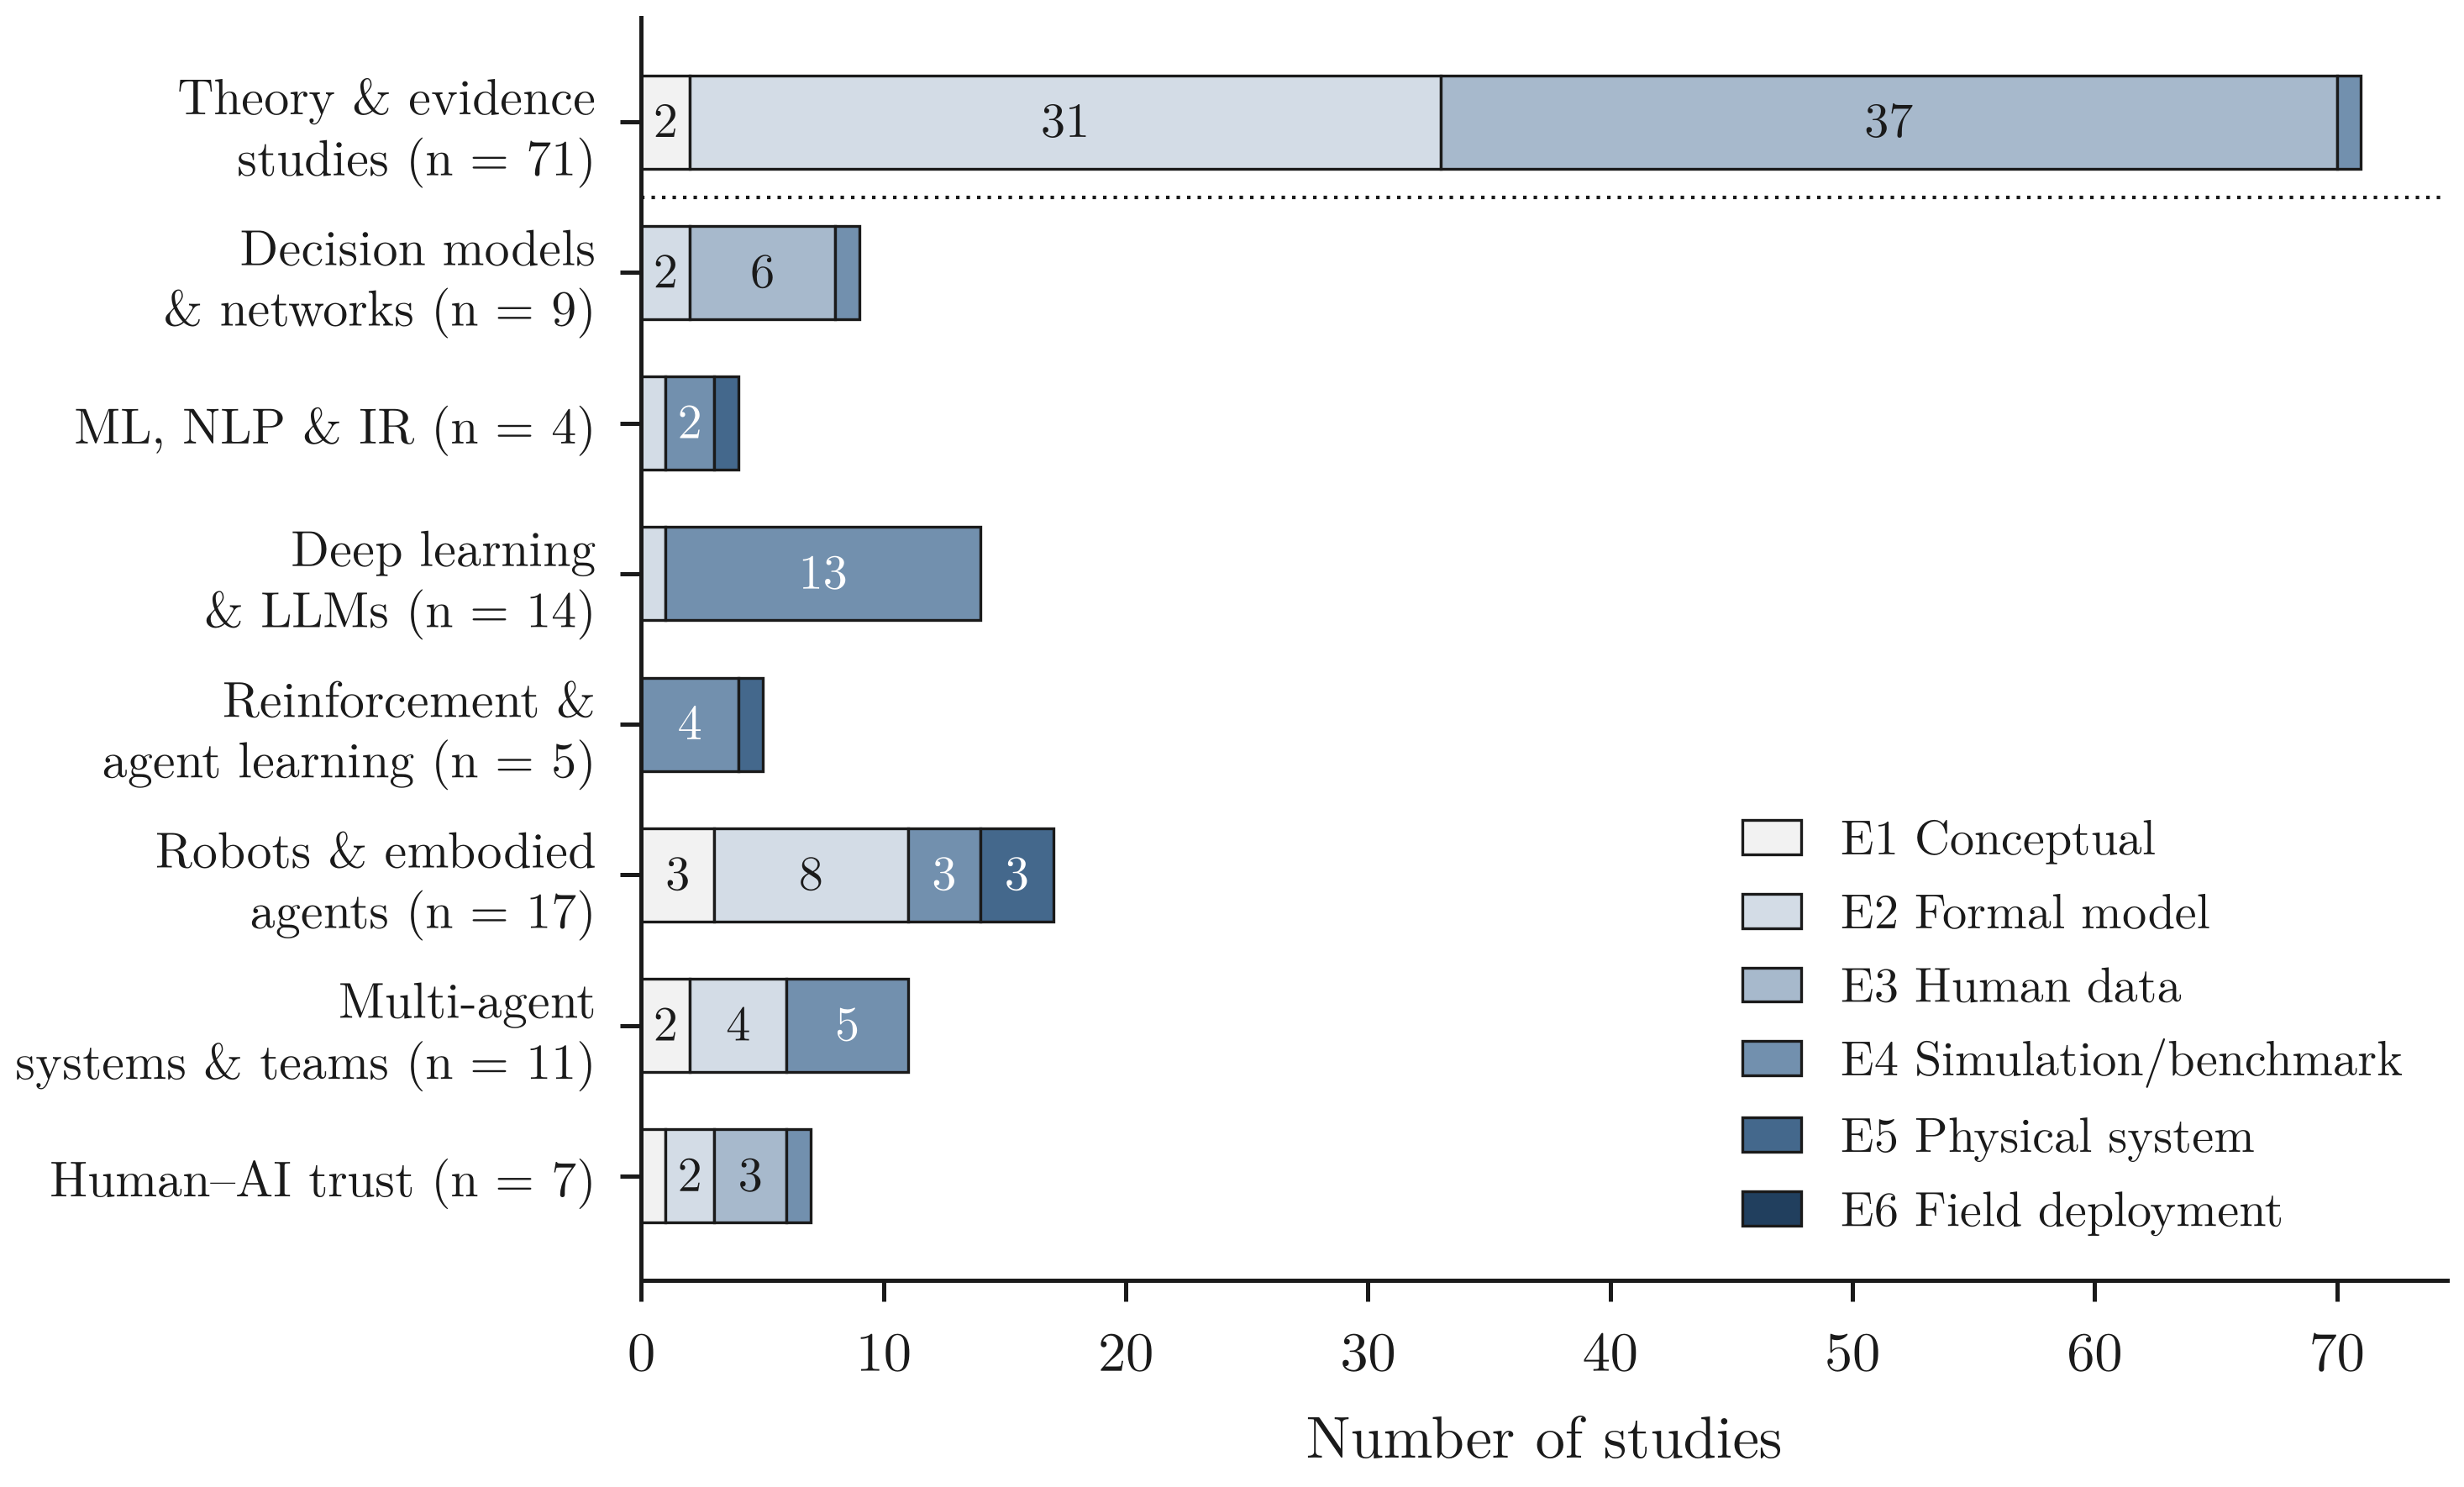
\includegraphics[width=0.95\textwidth]{figures/Fig7_evidence.png}
\caption{Evidence levels of the 138 graded studies in the corpus: the 71 theory and evidence studies (top bar) and the 67 application studies by domain (reviews and background works are not graded). E1 conceptual; E2 formal model; E3 human data; E4 simulation or benchmark; E5 physical system; E6 field deployment. No study reaches E6}\label{fig:evidence}
\end{figure}

\paragraph{Human--AI trust and oversight} Human trust in automation is the application domain in which quantum-like models have the strongest human-data support. Quantum models outperformed Markov models in predicting how people's reliability judgements of an automated system evolve over an interaction~\citep{Roeder2023}, and a quantum-inspired model was fitted to air-traffic controllers' trust in automation, although with a very small sample~\citep{Pushparaj2021}. Quantum-like trust models have been proposed for AI-supported decisions, including military decision aids~\citep{Humr2023,Humr2025,Humr2026}, and quantum random walks with interaction-dependent Hamiltonians have been fitted to the reliability ratings of 34 participants who worked with an AI image classifier~\citep{vanderMeer2025}; computational trust between artificial agents has also been given a quantum-like formulation~\citep{Ashtiani2019}. These models share a common structure: the person's trust is a state that is changed by each interaction, so the order in which the agent presents advice, explanations and errors becomes a design variable. For autonomous systems, the practical uses are to anticipate when a person's reliance will shift, to choose the order and framing of explanations, and to trigger escalation to human oversight before trust and system capability diverge (Section \ref{sec:safety}). None of these models has yet been evaluated in closed loop with a robot.

\paragraph{Quality of the application studies} The appraisal (Online Resource 1, Table S5) shows where the evidence is weakest. Model specification is the strongest criterion: 47 of the 61 appraised studies state their state space, operators and parameters in full. A classical model was evaluated on the same task in only 24 of the 61, partly in 16, and not at all in 21. Twenty-seven of the 61 give no a priori constraint on their free parameters, typically the interference phases, and validate them on no held-out data; 18 do. Empirical grounding is split: 19 studies use human data or a realistic agent or AI task, 24 use a narrow benchmark or aggregate data from a few classic paradigms, and 18 use toy examples or no data. Of the 14 studies whose code and data statements we could check, 5 released code or data in full or in part. Seven studies discuss their limitations and classical alternatives in depth; most do so briefly.

\subsection{Unique Contribution of This Survey}\label{sec:contrib}
To our knowledge, this review is the first to make the following six contributions.

\begin{enumerate}
\item It is the first systematic review, reported to PRISMA 2020, of quantum-cognition models applied to autonomous agents, with every judgement published as data (Section \ref{sec:method} and Online Resources 1, 3 and 4).
\item It connects the psychological evidence base to applications in robotics, reinforcement learning, machine learning and deep learning, large language models and human--AI trust within one framework (Sections \ref{sec:theory}--\ref{sec:multi}).
\item It separates quantum-like, quantum-inspired and quantum-circuit work consistently throughout.
\item It grades every application study on a six-level evidence scale, from conceptual proposals to field deployment, and appraises each against seven quality criteria.
\item It confronts the applications with the critical literature and with classical competitors (Sections \ref{sec:evidence} and \ref{sec:compare}).
\item It provides case studies, an illustrative experiment, a decision guide, a validation roadmap, a benchmark suite and a replication checklist, with reproducible code (Sections \ref{sec:cases}, \ref{sec:validation} and \ref{sec:bench}, Appendix \ref{app:code} and Online Resource 2).
\end{enumerate}


%% -----------------------------------------------------------------------------
\section{Head-to-Head Comparison --- Quantum vs. Classical (Honest Trade-offs)}\label{sec:compare}
Table \ref{tab:compare} summarises the comparison of quantum-like and classical approaches.

\begin{table}[ht]
\caption{Comparison of classical and quantum-like or quantum-inspired approaches}\label{tab:compare}%
\footnotesize
\begin{tabular}{@{}>{\raggedright\arraybackslash}p{0.200\dimexpr\textwidth-8\tabcolsep\relax}>{\raggedright\arraybackslash}p{0.250\dimexpr\textwidth-8\tabcolsep\relax}>{\raggedright\arraybackslash}p{0.270\dimexpr\textwidth-8\tabcolsep\relax}>{\raggedright\arraybackslash}p{0.280\dimexpr\textwidth-8\tabcolsep\relax}@{}}
\toprule
\textbf{Criterion} & \textbf{Classical (Bayes, Markov, DRL)} & \textbf{Quantum-like or quantum-inspired} & \textbf{Current evidence} \\ \midrule
Order and context effects & Require extra mechanisms (anchoring, memory) & Arise from non-commuting projectors; a priori QQ constraint & Strong for QQ~\citep{Wang2014}; classical accounts possible~\citep{Kellen2018} \\
Total-probability violations & Cannot be produced without changing the model & Interference terms & Replicated in two-stage tasks~\citep{Wang2016,Kvam2015} \\
Conjunction fallacy & Noise models (probability theory plus noise) & Sequential projection & Contested~\citep{BoyerKassem2016,Costello2018} \\
Dynamics of belief and trust & Markov random walks & Quantum walks, open systems & Mixed: quantum better at low coherence~\citep{Busemeyer2019}; trust~\citep{Roeder2023} \\
Physical state estimation & Kalman and particle filters (optimal) & No advantage expected & No comparison published \\
Classification accuracy & Strong deep-learning baselines & Parity on benchmarks & \citep{Li2019,Li2021b} \\
RL performance & Tuned deep RL, scalable & QiRL robust to learning rate; unstable under reward noise & No better policies~\citep{Dong2012}; Section \ref{sec:rl-exp} \\
Parameters and flexibility & Well understood & Phases and instruments add flexibility & Risk of over-fitting~\citep{Broekaert2017} \\
Interpretability & Varies & Geometric parameters; untested with users & No user studies \\
Hardware needs & CPU or GPU & CPU or GPU (quantum-like); QPU optional & Few-qubit demonstrations~\citep{Widdows2023} \\
\botrule
\end{tabular}
\end{table}

\subsection{Quantum Cognition vs. Bayesian Networks}

\subsubsection{When Classical Wins: Simple, Well-Defined Domains}
When all variables are compatible (jointly measurable, context-free), QP reduces to classical probability and adds only parameters~\citep{Bruza2015}. For physical state estimation, diagnosis from calibrated sensors~\citep{Blanke2016} and planning with known dynamics, Bayesian networks and filters are simpler, better understood and supported by mature tooling. Markov models remain adequate for most participants in several dynamic tasks~\citep{Busemeyer2019,Epping2023}.

\subsubsection{When Quantum Wins: Non-Commutative Measurements and Interference}
QP models win where their a priori structure matches the phenomenon: question-order effects that obey the QQ equality~\citep{Wang2014}, total-probability violations in two-stage decisions~\citep{Pothos2009,Wang2016} and interference of choice on confidence~\citep{Kvam2015}. In direct comparisons, Hilbert-space multidimensional models compared favourably with Bayesian networks~\citep{Busemeyer2018} and quantum-like influence diagrams predicted paradoxical choices that expected utility cannot~\citep{Moreira2020b}. The main classical competitors are noisy classical reasoning~\citep{Costello2014,Costello2018}, classical accounts of mirrored order effects~\citep{Kellen2018} and contextuality analyses that attribute effects to direct influences~\citep{Dzhafarov2016b}. Replies and new tests continue~\citep{Busemeyer2017b,Basieva2019}.

\subsection{Quantum Cognition vs. Deep Reinforcement Learning}

\subsubsection{Classical DRL: Scalable but Data-Hungry}
Deep RL scales to high-dimensional robot control but requires large amounts of data and careful tuning, and its reported gains are fragile~\citep{Henderson2018}.

\subsubsection{Quantum RL: Cheap and Parameter-Efficient, but Not Yet Better}
Quantum-inspired RL is cheap and can be robust to learning-rate choices~\citep{Dong2012}, but our illustrative experiment shows instability under reward noise (Section \ref{sec:rl-exp}). Circuit-based RL is parameter-efficient on benchmark tasks but not yet better or faster in wall-clock terms~\citep{Skolik2022,Jerbi2021,Meyer2022}, as the companion survey also concludes for robots~\citep{Guru2026}. The claim that quantum RL is more interpretable is not supported by any user study we found.

\subsection{Quantum Cognition vs. Transformer Attention Models}\label{sec:vs-attention}

\subsubsection{Attention as Soft Measurement: Order Effects in Transformers}
Attention weights a set of tokens by their compatibility with a query, loosely analogous to a context-dependent measurement. The analogy is suggestive, and QP tools (the QQ equality, contextuality-by-default) are useful auditing instruments for LLMs~\citep{Lo2025,Kang2026}. However, transformers are classical functions of their input; order effects in LLMs can arise from training data and position encodings without any QP structure, and their human-likeness varies across models and prompts~\citep{Tjuatja2024,Imannezhad2026}. QP models are best used here to describe and test LLM behaviour, not as a claim about its mechanism.

\subsection{Hybrid Approach: When to Use Each}\label{sec:guide}
Figure \ref{fig:guide} condenses the comparison into a decision guide. Keep a classical core for perception, estimation and control, where classical methods are optimal or nearly so. Add a quantum-like module only where the agent must predict, explain or align with judgements that are sequential, ambiguous or context-dependent. Typical cases are human intentions, trust and preferences, and the answers of other learned agents. Validate the module against a classical model with the same number of parameters and against a noise-augmented classical model.

\begin{figure}[ht]
\centering
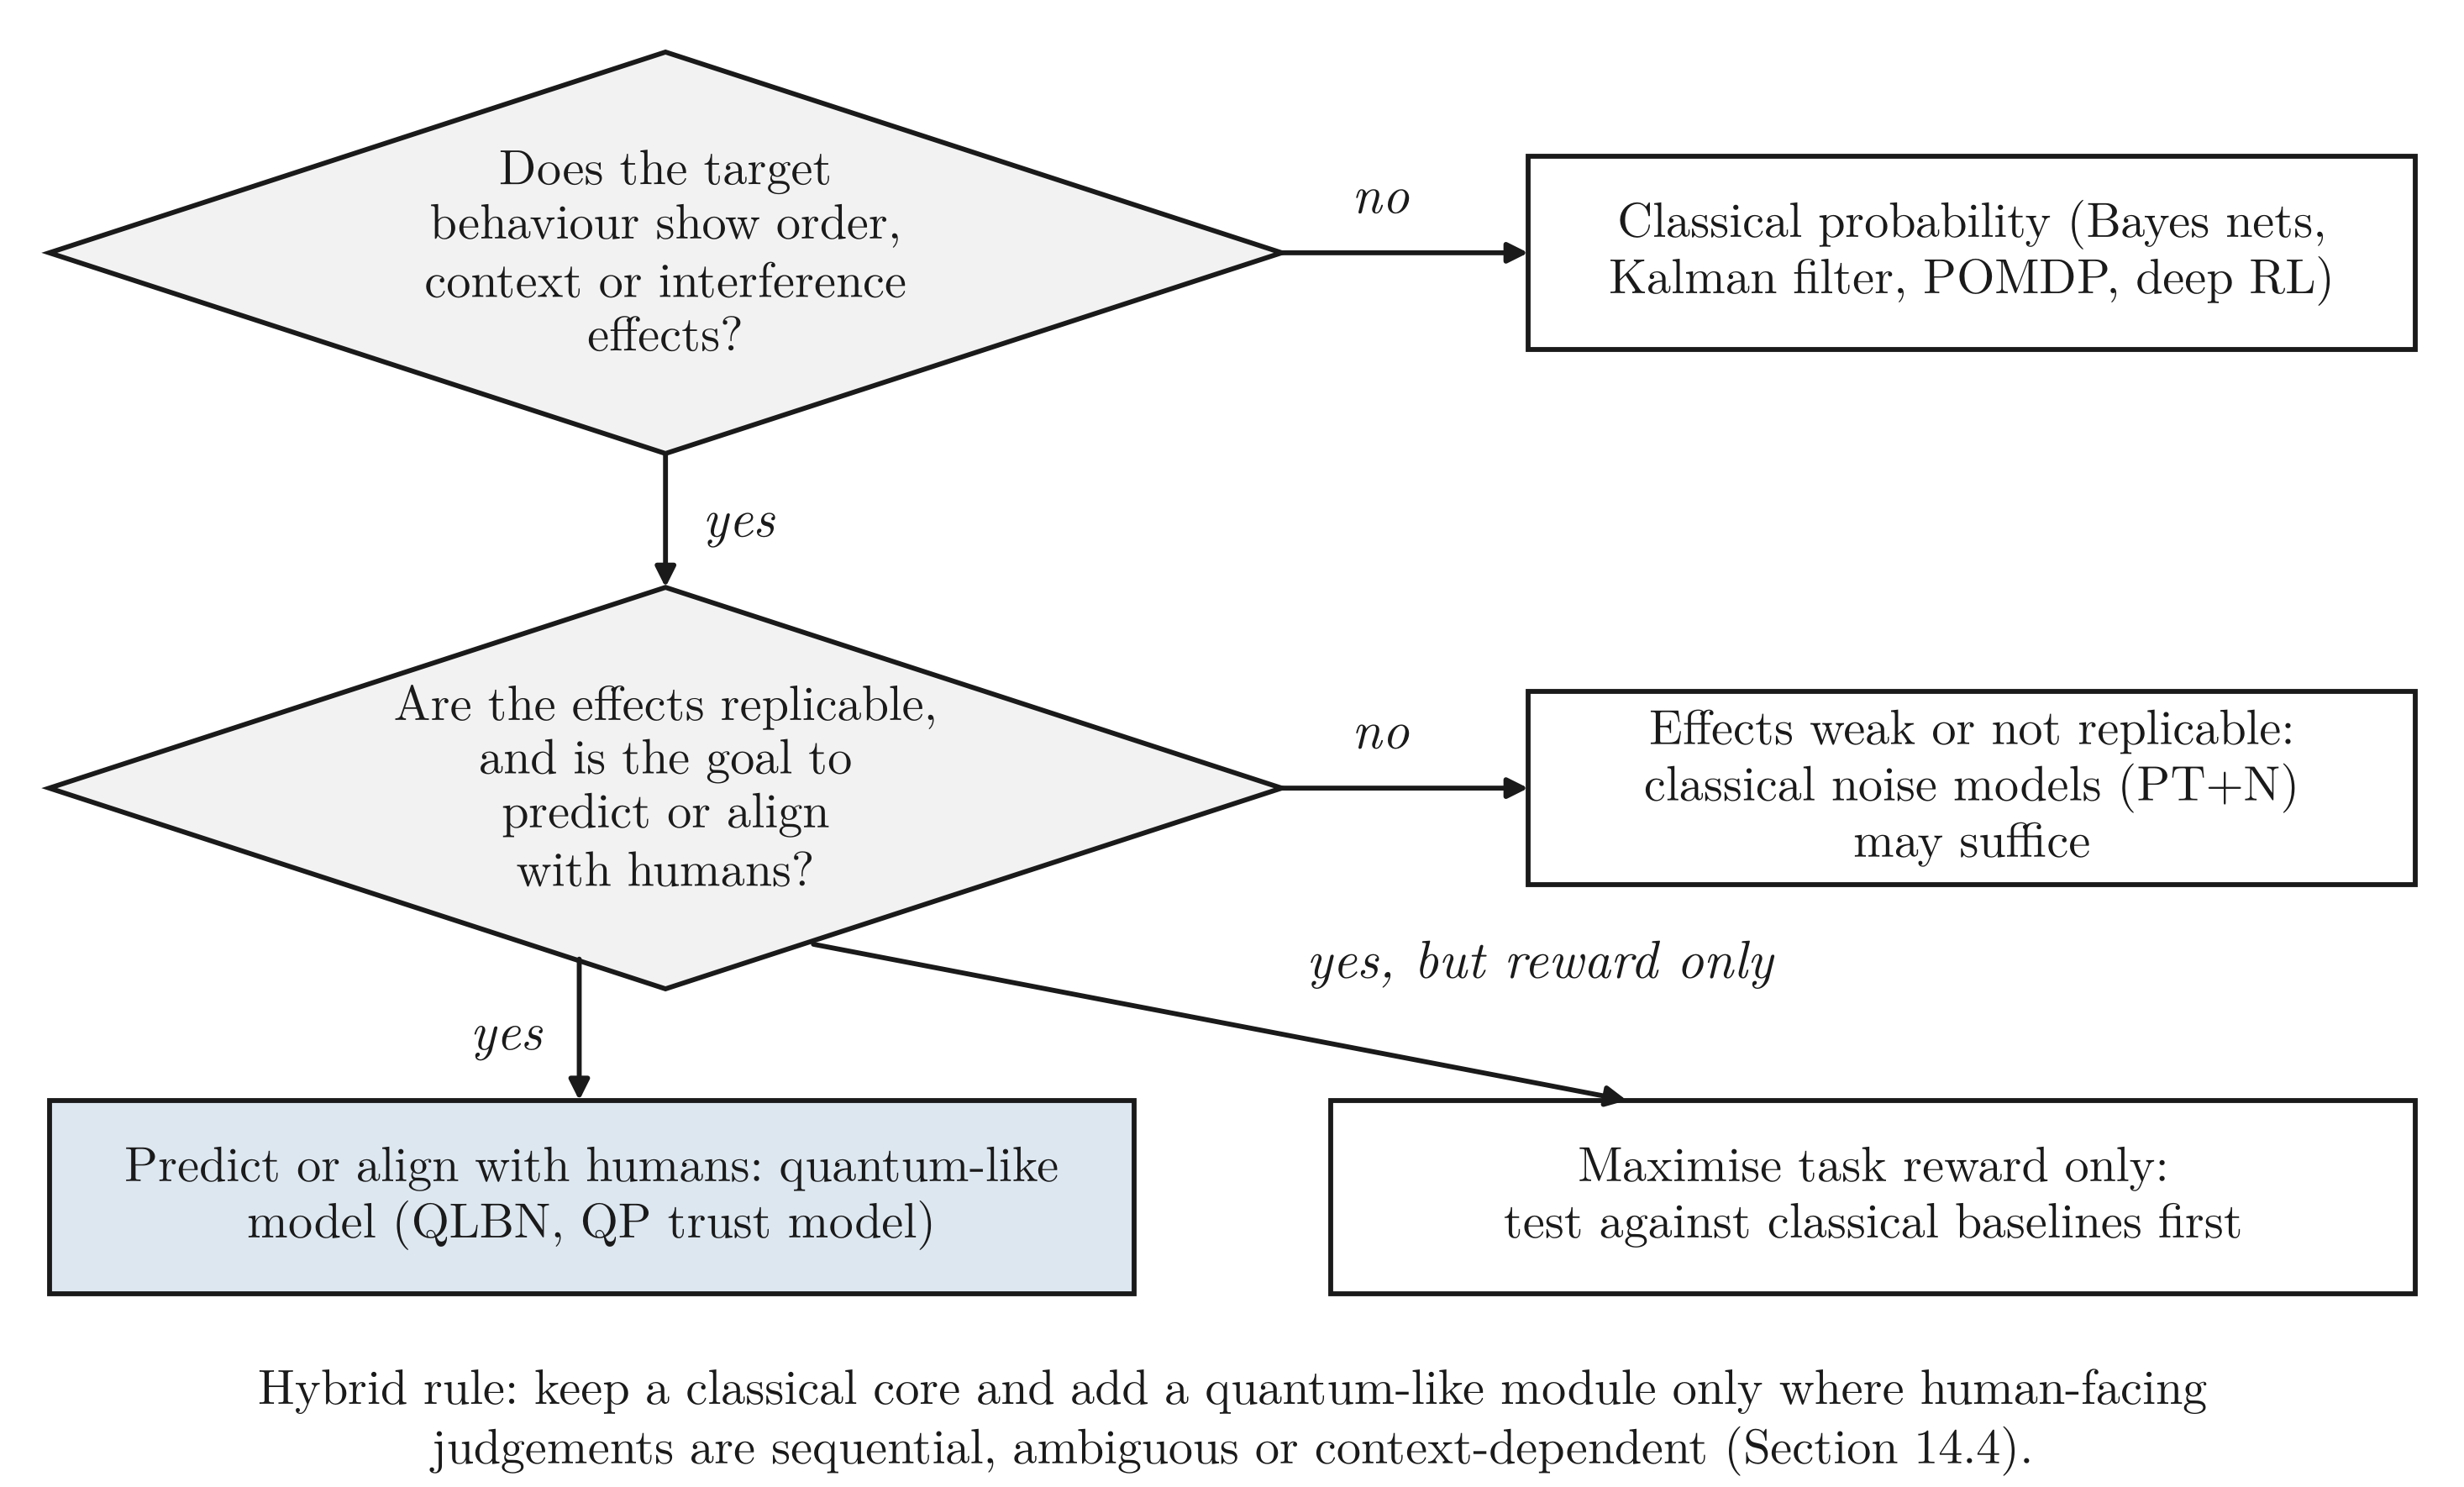
\includegraphics[width=0.95\textwidth]{figures/Fig8_decision_guide.png}
\caption{Decision guide for choosing between classical and quantum-like models in an autonomous system}\label{fig:guide}
\end{figure}


%% -----------------------------------------------------------------------------
\section{Experimental Validation Roadmap}\label{sec:validation}
Sections \ref{sec:validation}, \ref{sec:bench} and \ref{sec:directions} have distinct roles: this section states which experiments are needed, Section \ref{sec:bench} specifies the benchmarks and reporting standard for running them, and Section \ref{sec:directions} lists the open research problems that remain beyond them. Because the literature contains almost no controlled comparisons on autonomous systems, we propose a two-phase validation programme. Each task has a classical baseline, a quantum-like model and an a priori QP prediction that can fail.

\subsection{Phase 1 (Simulation): Benchmark Tasks}

\subsubsection{Task 1: Fault Diagnosis in Simulated Autonomous Systems}
A simulated mobile robot with injected faults receives diagnostic evidence from heterogeneous sources (sensor residuals, operator reports, log classifiers) presented in different orders. The baseline is a Bayesian-network or observer-based diagnoser~\citep{Blanke2016}. The test is whether a QLBN predicts operators' order-dependent diagnoses better, and whether exploiting it improves joint human--robot diagnosis accuracy. The quantum fault-tolerant filter~\citep{Gao2021} is not an appropriate baseline because it addresses quantum systems.

\subsubsection{Task 2: Multi-Sensor Fusion Under Ambiguity}
Fusion of physical sensors (baseline: Kalman or particle filter) combined with semantic cues from language or human reports. The prediction is that QP fusion helps only in the semantic, context-dependent channel; it should do no better than the Kalman filter on physical channels (Section \ref{sec:case-fusion}).

\subsubsection{Task 3: Navigation and Decision-Making with Conflicting Information}
Navigation where route advice from a human, a map and a learned model conflict. Baselines are POMDP planners and ensembles; the quantum-like model predicts the human's acceptance of advice as a function of order and framing~\citep{Song2022,Roeder2023}.

\subsubsection{Task 4: ML/DL Classification Under Label Ambiguity}
Classification of ambiguous images, with human labels collected under controlled question orders. The model predicts order-dependent label distributions and the QQ statistic; the baseline is a calibrated softmax classifier with annotator noise.

\subsection{Phase 2 (Real Systems): Hardware Validation}

\subsubsection{Robotic Platforms: Grasping, Manipulation, Navigation}
Human--robot handover, shared manipulation and guided navigation are natural platforms because a human judgement is embedded in the loop. The primary outcome is task success and human trust, not model fit alone.

\subsubsection{Real-World AI/ML Systems: Object Recognition, Intent Prediction}
Decision-support systems in which people accept or reject AI recommendations, as in air-traffic control~\citep{Pushparaj2021} or military decision aids~\citep{Humr2026}, offer realistic settings with measurable trust dynamics. Pedestrian-intent prediction for automated driving~\citep{Song2022} and object recognition with human-labelled ambiguous categories are the corresponding perception tasks.

\subsection{Metrics and Baselines}\label{sec:metrics}
Table \ref{tab:metrics} lists the metrics. Every study should report predictive accuracy on held-out data (not only fit), model complexity (parameters, AIC/BIC or cross-validated likelihood), a parameter-matched classical baseline, a noise-augmented classical baseline such as probability theory plus noise~\citep{Costello2014}, and at least one a priori QP test (the QQ equality, a total-probability test or a contextuality test with direct influences controlled)~\citep{Dzhafarov2016a}. The appraisal of Section \ref{sec:map} shows that most published applications fall short on exactly these points.

\begin{table}[ht]
\caption{Metrics and baselines for validating quantum-like models in autonomous systems}\label{tab:metrics}%
\footnotesize
\begin{tabular}{@{}>{\raggedright\arraybackslash}p{0.320\dimexpr\textwidth-6\tabcolsep\relax}>{\raggedright\arraybackslash}p{0.340\dimexpr\textwidth-6\tabcolsep\relax}>{\raggedright\arraybackslash}p{0.340\dimexpr\textwidth-6\tabcolsep\relax}@{}}
\toprule
\textbf{Metric} & \textbf{What it measures} & \textbf{Why it is needed} \\ \midrule
Held-out predictive log-likelihood & Out-of-sample prediction of human or agent judgements & Avoids rewarding flexible models that only fit \\
AIC, BIC and parameter count & Model complexity & QP phases and instruments add freedom \\
QQ statistic or total-probability test & An a priori QP prediction & Makes the QP model falsifiable \\
Contextuality-by-default with direct influences & Genuine contextuality & Separates contextuality from signalling \\
Task success, return or error & Autonomous-system performance & The outcome that matters for deployment \\
Trust and acceptance & Human reliance on the agent & Main target of human-facing QP models \\
Seeds and confidence intervals & Statistical robustness & RL results are seed-sensitive \\
Latency and compute & Real-time feasibility & Embedded deployment \\
\botrule
\end{tabular}
\end{table}


%% -----------------------------------------------------------------------------
\section{Case Studies and Worked Examples}\label{sec:cases}
Case Studies 1 and 2 are worked numerical examples that show what a QP model computes and predicts; they are not experiments and report no performance results. Case Study 3 is a small illustrative experiment. All three use the code in Appendix \ref{app:code} (Online Resource 2); their numerical values are collected in Appendix \ref{app:exp}.

\subsection{Case Study 1: Pose Estimation from Noisy Multimodal Sensors}\label{sec:case-fusion}

\subsubsection{Problem Setup}
A robot estimates its position along a corridor from two sensors, a lidar reading $z_1 = 2.10$ m (variance 0.04) and a camera estimate $z_2 = 1.90$ m (variance 0.09). A human operator also reports whether the robot has ``passed the doorway'', and a vision classifier gives its own judgement.

\subsubsection{Classical Approach (Kalman Filter)}
The Kalman update gives $\hat{x} = 2.038$ m with variance 0.028 m$^2$, and the result is identical whichever sensor is processed first~\citep{Kalman1960}. For this physical sub-problem, the Kalman filter is optimal and a QP model cannot improve on it.

\subsubsection{Quantum Cognition Approach}
The QP model is applied only to the semantic judgement ``has the robot passed the doorway?'', which combines two context-dependent cues: the operator's report ($p = 0.80$ of ``passed'' when that cue is attended) and the classifier's judgement ($p = 0.30$). With equal weights the classical mixture is 0.55. A QLBN adds an interference term $2\sqrt{0.5 \cdot 0.80 \cdot 0.5 \cdot 0.30}\,\cos\theta = 0.49\cos\theta$, giving 0.55 at $\theta = 90$\textdegree{} (the classical case), 0.795 at $\theta = 60$\textdegree{} and 0.305 at $\theta = 120$\textdegree{}; at $\theta = 0$ the unnormalised value exceeds 1, which is why QLBNs must renormalise~\citep{Moreira2016,Wichert2020}. The phase encodes how the two cues interact in the human's judgement, and it must be estimated from, or better predicted for, human data.

\subsubsection{Results and Comparison: What the Worked Example Shows}
The worked example shows the correct division of labour: physical fusion stays classical, and QP models the human-facing judgement. We found no published study that compares QP and classical fusion on robot pose estimation, and we do not expect QP to help there.

\subsection{Case Study 2: Image Classification Under Label Ambiguity (ML/DL)}\label{sec:case-label}

\subsubsection{Problem Setup: Objects with Multiple Valid Labels}
An image of a large domestic-looking cat is judged by annotators on two questions: ``cat?'' and ``wild animal?''. Human answers to such overlapping categories are order-dependent~\citep{Wang2016}.

\subsubsection{Classical Approach (CNN + Softmax)}
A CNN with independent sigmoid outputs~\citep{Krizhevsky2012} predicts $p(\text{cat})$ and $p(\text{wild})$ and, if a joint is needed, assumes conditional independence. The joint probability is the same whichever question is asked first.

\subsubsection{Quantum Cognition Approach}
Represent the image as a state at 35\textdegree{} in a two-dimensional judgement space, with ``cat'' at 0\textdegree{} and ``wild'' at 60\textdegree{}. Then $p(\text{cat}) = 0.671$ and $p(\text{wild}) = 0.821$; $p(\text{cat, then wild}) = 0.168$ but $p(\text{wild, then cat}) = 0.205$. The model predicts a specific order effect and, through the QQ equality, a constraint on the four sequential answer patterns that can be tested on annotation data.

\subsubsection{Results: Predicted Order Effects Rather than Accuracy Gains}
No accuracy gains are claimed. The value of the QP model is that it predicts the order-dependence of human labels, which a softmax classifier cannot represent; whether modelling this improves learning from human labels is untested and is the purpose of Benchmark 3 (Section \ref{sec:bench}).

\subsection{Case Study 3: RL Policy Learning Under Reward Uncertainty}\label{sec:rl-exp}

\subsubsection{Problem Setup: Ambiguous Reward Signals}
A tabular agent must reach the goal of a $6 \times 6$ grid with four internal walls (shortest path: 10 steps). Reaching the goal gives reward $+1$ and each step $-0.01$. In the noisy condition, Gaussian noise ($\sigma = 0.5$) is added to every reward. Each agent is trained for 300 episodes (maximum 200 steps each) with 30 random seeds.

\subsubsection{Classical Approach (Q-Learning)}
Because the state space is small, we use tabular Q-learning (learning rate 0.1, discount 0.95) with either $\varepsilon$-greedy exploration ($\varepsilon$ decaying from 0.3 to 0.01) or softmax exploration (temperature decaying from 0.2 to 0.01). Deep Q-learning would behave similarly on this task at much higher cost.

\subsubsection{Quantum RL Approach}
The quantum-inspired agent follows Dong et al.'s QRL~\citep{Dong2008}: each state holds four action amplitudes (initially equal), actions are chosen by ``measurement'' with probability $|\text{amplitude}|^2$, state values are learned by TD(0), and the chosen action's amplitude is amplified by $L = \lfloor k(r + V(s')) \rfloor$ Grover iterations, capped at three, with $k = 30$ selected from $\{10, 30, 100\}$.

\subsubsection{Results and Convergence Analysis}
With deterministic rewards, all three agents learned the optimal 10-step path in every seed (Figure \ref{fig:rl}). The $\varepsilon$-greedy agent converged fastest (first episode at which the 10-episode moving average fell to 15 steps or fewer: $60 \pm 6$), while QRL ($134 \pm 20$) and softmax ($128 \pm 10$) were similar. With noisy rewards, QRL learned fastest at first: its median path length was 70 steps at episode 100, against 153 for $\varepsilon$-greedy and 200 (no progress) for softmax. However, it did not stabilise. Over the last 50 episodes its mean path length was $67 \pm 40$ steps, against $14 \pm 13$ for $\varepsilon$-greedy and $16 \pm 17$ for softmax, and 5 of 30 seeds never met the convergence criterion. Varying $k$ did not remove the instability (final means of 78, 67 and 74 steps for $k = 10$, 30 and 100). The reason is structural: amplitude amplification only increases the probability of rewarded actions, so an action amplified by a noisy positive reward is never de-amplified. The experiment is small and illustrative: one tabular task, one quantum-inspired variant and two simple classical baselines, so it is not a benchmark and does not show that quantum-inspired RL is generally worse; a fair evaluation would use the protocol of Benchmark 4. It does show why quantum-inspired RL must be compared with tuned classical baselines under realistic noise, and it points to a concrete design fix: amplitude updates that can also decrease (Appendix \ref{app:ext}). Full results are in Appendix \ref{app:exp}.

\begin{figure}[ht]
\centering
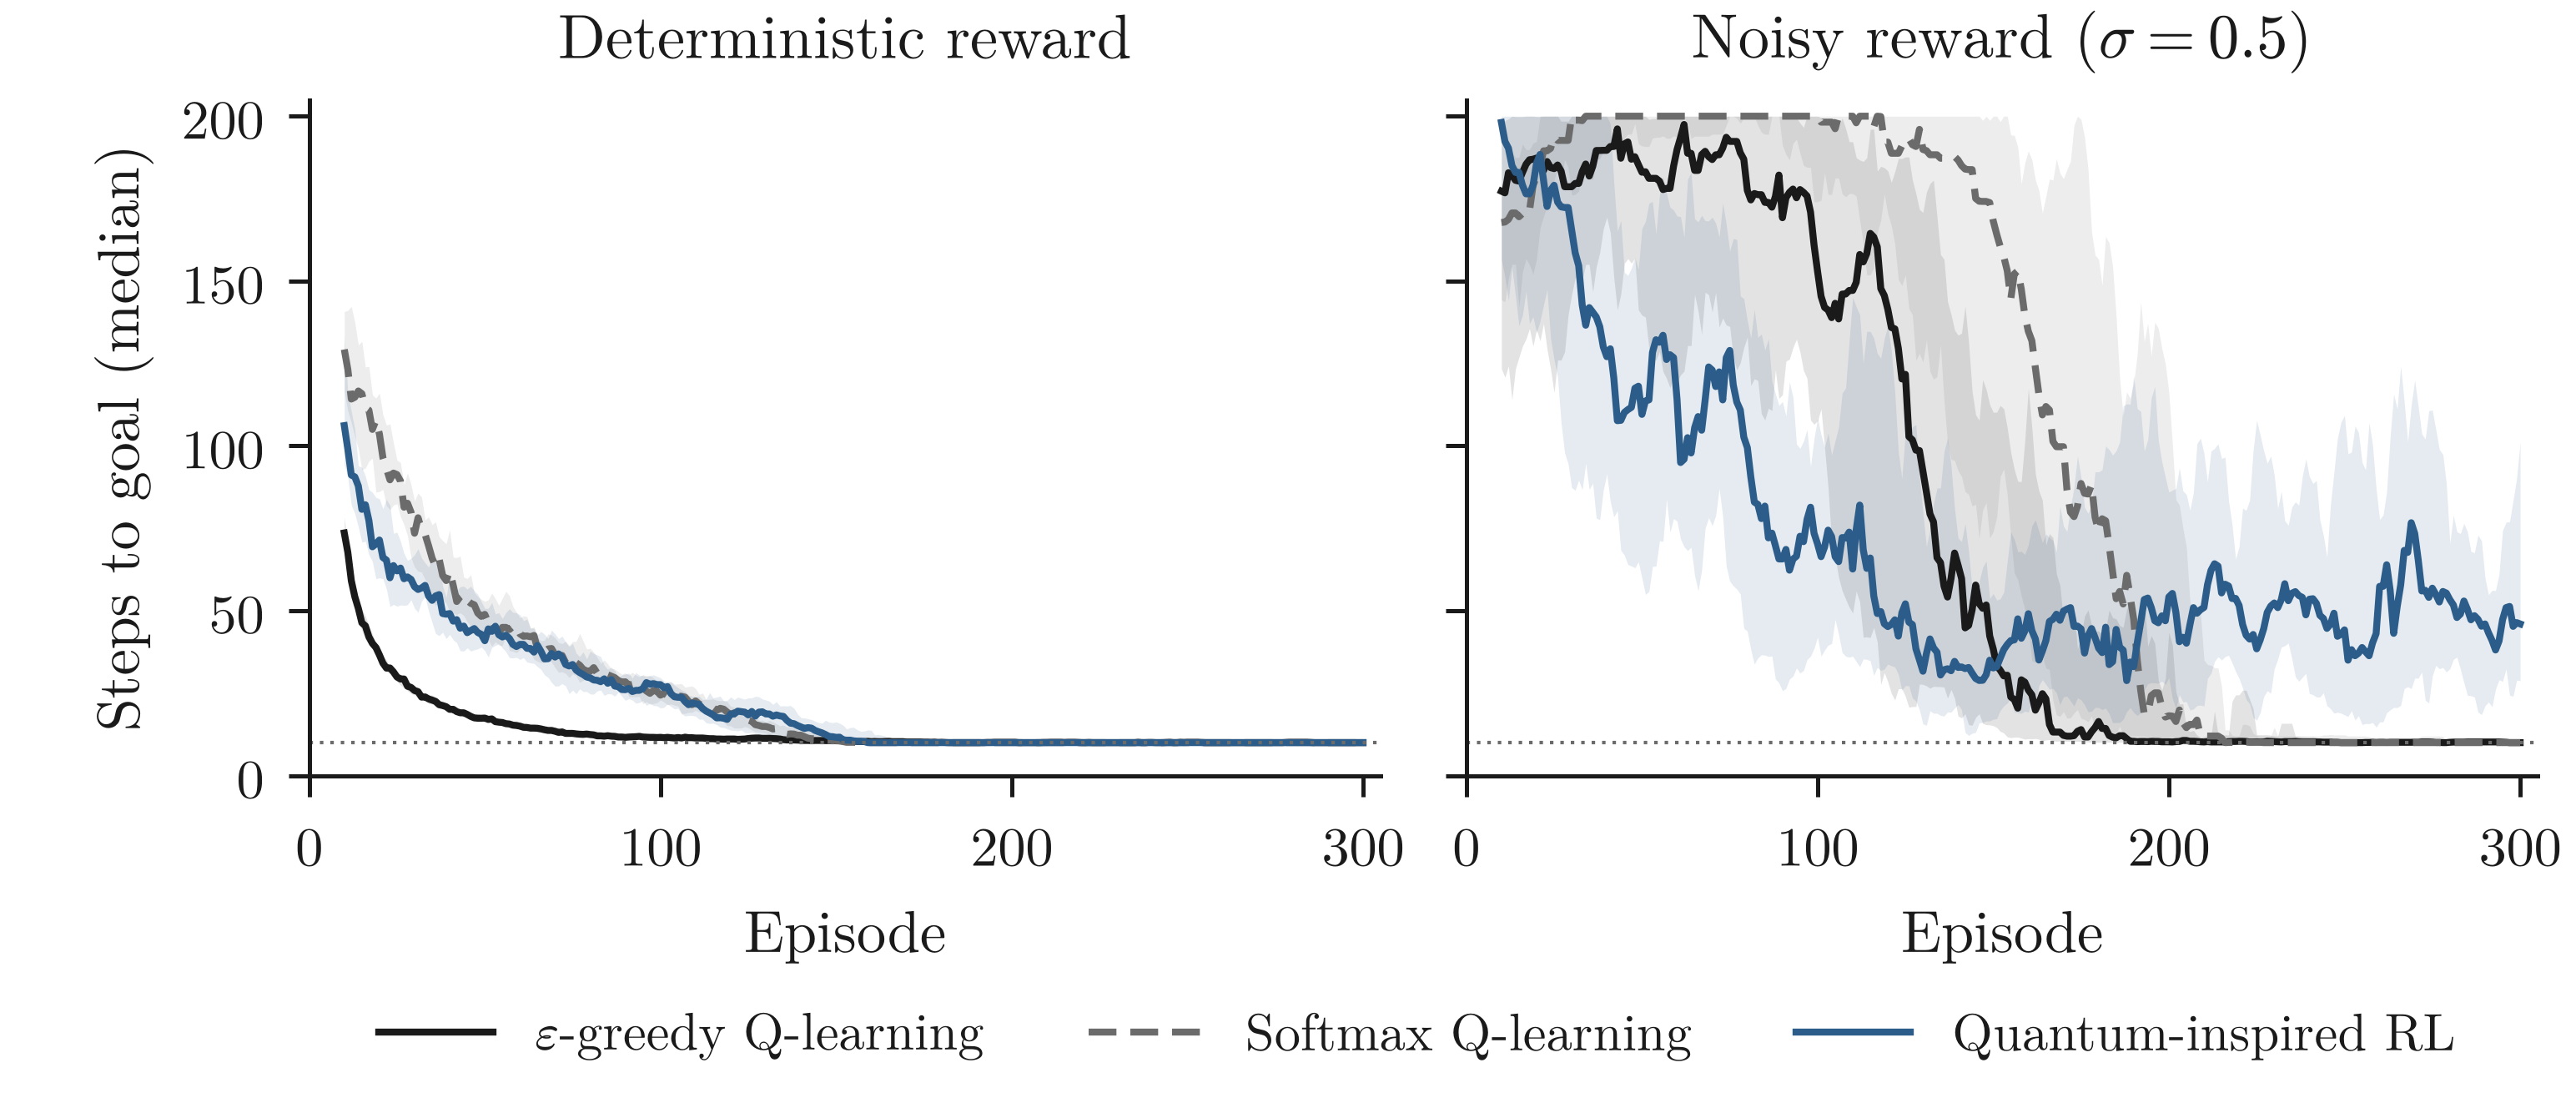
\includegraphics[width=1.00\textwidth]{figures/Fig9_rl.png}
\caption{Case Study 3: steps to reach the goal in a $6 \times 6$ grid for $\varepsilon$-greedy Q-learning, softmax Q-learning and quantum-inspired RL (Dong et al. 2008), with deterministic (left) and noisy (right) rewards. Lines show the median of 30 seeds of the 10-episode moving average; shading shows the interquartile range; the dotted line is the optimal path length. Experiment run for this review (code in Online Resource 2)}\label{fig:rl}
\end{figure}


%% =============================================================================
\surveypart{Part D --- Grounding and Implications (Sections 17--20)}

\section{Limitations and Failure Modes}\label{sec:limits}

\subsection{When Quantum Cognition Does Not Help}\label{sec:nohelp}
QP models do not help when all relevant variables are compatible, which covers most physical sensing, estimation and control; the models then reduce to classical probability with extra parameters~\citep{Bruza2015}. They do not help when the target effects are weak or absent in the population of interest: several conjunction-fallacy predictions failed~\citep{BoyerKassem2016}, classical noise models explain many judgement biases~\citep{Costello2014,Costello2018}, and in dynamic tasks many participants are fitted as well by Markov models~\citep{Epping2023}. Nor do they help when the goal is simply to maximise an agent's task reward, where no study has shown a QP decision module outperforming a tuned classical one. Finally, they do not help when the effects are artefacts of the measurement interface, for example saturated LLM outputs that render the QQ test uninformative~\citep{Kang2026}.

\subsection{Interpretability Challenge: ``Black Box'' Superpositions}\label{sec:interp}
QP models are often described as interpretable because their parameters are geometric (angles between subspaces, phases). In practice, complex phases and high-dimensional density matrices are no easier for users to understand than neural weights, and interpretability claims for quantum-inspired networks have not been tested with users~\citep{Li2019,Li2021b}. Interpretable quantum ML is an active research goal rather than an achievement~\citep{Flamini2024}.

\subsection{Computational Overhead vs. Accuracy Gain}\label{sec:compute}
Quantum-like models are cheap at the scale of psychological experiments but scale exponentially if every binary variable becomes a qubit (Section \ref{sec:hw}). Quantum-hardware versions add queueing, noise and barren plateaus~\citep{Preskill2018,Cerezo2021}, and dequantisation shows that some claimed quantum speed-ups vanish against clever classical algorithms~\citep{Tang2019,Aaronson2015}. Where accuracy gains have been measured, they are typically parity or small improvements on benchmarks (Sections \ref{sec:ml}--\ref{sec:rl}).

\subsection{Real-Time Constraints in Robotics and Embedded AI}\label{sec:realtime}
A two- to eight-dimensional QP model can be evaluated in microseconds on an embedded CPU, so quantum-like decision modules are compatible with real-time control. Circuit-based implementations on cloud quantum processors are not: queueing and communication latencies are orders of magnitude larger than control cycles. Real-time use therefore implies classical simulation of the QP model.


%% -----------------------------------------------------------------------------
\section{Assumptions and Caveats}\label{sec:assumptions}

\subsection{Core Assumptions: Linearity, Finite Dimensionality, Closure}
QP models assume that belief states form a linear space, that a finite (usually small) dimension suffices, and that measurement outcomes are closed under the chosen projectors or instruments. Dynamic models further assume a specific Hamiltonian or Lindblad generator~\citep{Busemeyer2020,Asano2026}.

\subsection{Where These Assumptions May Break Down}
Response replicability shows that simple projective models are too restrictive~\citep{Khrennikov2014}; quantum instruments fix this at the cost of extra flexibility~\citep{Ozawa2020,Ozawa2021}. Some order-effect data appear to be non-Hilbertian altogether~\citep{Aerts2017b}. Signalling (direct influence of context on marginal probabilities) violates the assumptions under which Bell-type and contextuality tests are interpreted~\citep{Dzhafarov2016a}. Individual differences are often averaged away in aggregate fits~\citep{Epping2023}.

\subsection{Uncertainty and Knowledge Gaps}
Key unknowns for autonomous systems are: whether QP effects in laboratory tasks generalise to operational settings; how to set phases a priori rather than fit them~\citep{Wichert2020}; how QP models should be learned from data at scale; and whether modelling human QP effects improves joint human--agent performance. A further source of uncertainty for this review is that 51 of the 67 application studies were extracted from their abstracts, and several recent preprints have not yet been peer-reviewed (Section \ref{sec:classification}).


%% -----------------------------------------------------------------------------
\section{Ethical, Safety and Transparency Implications}\label{sec:ethics}

\subsection{Transparency: Can We Explain Quantum Decisions in AI/ML?}\label{sec:transparency}
A QP decision module can be explained in terms of its elements: which questions were asked, in which order, and how each answer changed the state. This is a potential transparency advantage over opaque neural policies, but it must be demonstrated with users. Designers should document the ordering of queries, because under QP the ordering is part of the decision.

\subsection{Safety: Escalation to Human Oversight}\label{sec:safety}
Quantum models of trust in AI provide the most direct safety application. They predict when human reliance will shift, which can trigger escalation or explanation~\citep{Roeder2023,Humr2025,Humr2026,vanderMeer2025}. Formal verification of autonomous robots remains classical~\citep{Luckcuck2019,Dreossi2019}; a QP module inside a verified system should be bounded by classical safety envelopes, so that its context-dependence cannot drive the system outside certified behaviour.

\subsection{Accountability: Who is Responsible When Autonomous Systems Fail?}\label{sec:accountability}
Because QP models make outcomes depend on the sequence of interactions, logs must record the order and framing of queries to allow audit. An order-dependent model that is not logged is effectively unaccountable, and responsibility for its failures then cannot be traced to a design decision.

\subsection{Bias and Fairness: Does Quantum Cognition Mitigate or Amplify Bias?}\label{sec:bias}
QP models reproduce human biases; that is their purpose in psychology. Used to predict people, they can help a system anticipate and correct for biased human inputs. Used to design an agent's own decisions, they risk importing those biases deliberately. The choice should be explicit: model human bias, do not emulate it, unless emulation is required for natural interaction and is disclosed. Tests of LLMs show that AI systems may display human-like biases, fewer biases or different biases depending on the model~\citep{Binz2023,Tjuatja2024,Imannezhad2026}.


%% -----------------------------------------------------------------------------
\section{Hardware and Implementation Requirements}\label{sec:hw}

\subsection{Classical Simulation Requirements}

\subsubsection{Memory Footprint (Exponential in Qubits)}
A pure state over $n$ binary variables needs $2^n$ complex amplitudes (16 bytes each in double precision): 16 KB for $n = 10$, 16 MB for $n = 20$ and 16 GB for $n = 30$. Density matrices square these figures. Practical cognitive models avoid this by using low-dimensional spaces per question set~\citep{Busemeyer2018} or tensor-network factorisations~\citep{Stoudenmire2016}.

\subsubsection{Computational Complexity and Scaling}
Applying a projector or a unitary costs $O(d^2)$ for a dense $d$-dimensional operator, and a Lindblad step costs $O(d^3)$. For the dimensions used in the literature ($d \leq 16$), these costs are negligible. QLBNs add a phase per unobserved node, so exact inference grows with the number of interference terms, as in classical exact inference~\citep{Moreira2014}.

\subsection{Real Quantum Hardware (Future)}

\subsubsection{Error Rates and Coherence Times}
Current noisy intermediate-scale devices~\citep{Preskill2018} suffice for the few-qubit circuits of cognitive models~\citep{Widdows2023}, but noise distorts sensitive order-effect circuits and adds latency. There is no computational need for hardware at these sizes; the companion survey quantifies the latency gap for robot control~\citep{Guru2026}.

\subsubsection{Qubit Connectivity and Topology}
Connectivity limits matter only for large entangled models, which cognitive models do not yet use. Quantum hardware becomes relevant only if QP models are scaled to many interacting variables or used as quantum-agent learners with proven speed-ups~\citep{Paparo2014,Saggio2021}.

\subsection{Practical Implementation: Software Stack and Frameworks (PyQuante, Qiskit, PennyLane)}\label{sec:software}
For quantum-like models, NumPy or SciPy suffices (Appendix \ref{app:code}), with QuTiP for open-system dynamics. For circuit implementations, Qiskit, PennyLane~\citep{Bergholm2018} and TensorFlow Quantum~\citep{Broughton2020} integrate with PyTorch and TensorFlow. PyQuante, named in some roadmaps, is a quantum-chemistry package and is not suited to cognitive modelling; we list it here only to prevent that mistake.


%% =============================================================================
\surveypart{Part E --- Integration and Future (Sections 21--25)}

\section{Connection to Neuroscience --- Is Quantum Cognition Biologically Grounded?}\label{sec:neuro}

\subsection{Do Brains Actually Use Quantum Mechanics?}
The Orch-OR theory proposes quantum computation in neuronal microtubules~\citep{Hameroff2014}, and Fisher proposed nuclear-spin qubits in Posner molecules as a possible quantum memory~\citep{Fisher2015}. Tegmark estimated that decoherence times in the brain are far shorter than neural processing times, making sustained quantum computation implausible~\citep{Tegmark2000}. These hypotheses are contested and are not required by quantum cognition.

\subsection{Predictive Processing as a Bridge}
Predictive processing and the free-energy principle cast cognition as prediction-error minimisation~\citep{Friston2010,Clark2013}. They provide a classical framework in which the constructive, context-dependent judgements that QP models describe could arise from hierarchical inference in which each query changes the prior for the next.

\subsection{Why Quantum Formalism Fits Behavioural Data (Without Requiring Quantum Brains)}
Several proposals show how classical neural systems could implement QP operations. Neural oscillators can realise unitary evolution, projection and state reduction~\citep{Busemeyer2017a}; uncertainty in neuronal firing can be represented as quantum-like superposition~\citep{Khrennikov2018}; and generalised probability theory links neuronal networks and oscillations to quantum-like cognition~\citep{Khrennikov2025a,Khrennikov2025b,Khrennikov2025c}. These are existence proofs rather than empirical findings, but they remove the need for a quantum brain.

\subsection{Implications for AI/ML and Robot Cognition Design}
If QP structure arises from classical mechanisms such as context-dependent sampling, oscillatory coding and constructive inference, artificial agents can reproduce it with classical computation. The design question is therefore not whether to use quantum hardware but whether an agent should represent incompatible perspectives explicitly, as QP models do.

Three design principles follow from the neural-implementation proposals. First, a judgement should be represented as a state relative to a basis chosen by the question, not as a fixed number stored for later retrieval; the oscillator account realises exactly this through the phase relation between populations~\citep{Busemeyer2017a}. Second, a decision should be modelled as a process that converges to a state, not as an instantaneous lookup; in the open-system account, decision-making is decoherence towards a steady state, with a convergence rate that the model makes explicit~\citep{Khrennikov2018}. Third, measurement should change the state: an agent that queries its own beliefs, or a person's, should update the queried state, which is the mechanism behind order effects. Each principle can be implemented in a classical neural network, and each yields a testable prediction about agent behaviour rather than about brains. Neuroscientific evidence would strengthen the case for QP models of people, but the case for using them in artificial agents rests on behavioural prediction alone.


%% -----------------------------------------------------------------------------
\section{Standardised Benchmarks and Reproducibility}\label{sec:bench}

\subsection{Proposed Benchmark Suite (Robotics, ML, RL, Physical AI)}
Table \ref{tab:bench} specifies four benchmarks that operationalise the validation roadmap (Section \ref{sec:validation}). Each pairs a classical baseline with an a priori QP test, so that a benchmark can falsify the QP model as well as support it. The full protocol is in Appendix \ref{app:protocols}.

\begin{table}[ht]
\caption{Proposed benchmark suite}\label{tab:bench}%
\footnotesize
\begin{tabular}{@{}>{\raggedright\arraybackslash}p{0.160\dimexpr\textwidth-10\tabcolsep\relax}>{\raggedright\arraybackslash}p{0.240\dimexpr\textwidth-10\tabcolsep\relax}>{\raggedright\arraybackslash}p{0.200\dimexpr\textwidth-10\tabcolsep\relax}>{\raggedright\arraybackslash}p{0.200\dimexpr\textwidth-10\tabcolsep\relax}>{\raggedright\arraybackslash}p{0.200\dimexpr\textwidth-10\tabcolsep\relax}@{}}
\toprule
\textbf{Benchmark} & \textbf{Task} & \textbf{Classical baseline} & \textbf{QP model and a priori test} & \textbf{Primary metrics} \\ \midrule
B1 Fault diagnosis & Simulated robot faults; operator judgements under order-randomised evidence & Bayesian network or observer-based diagnosis & QLBN; QQ test on paired questions & Diagnosis accuracy; held-out likelihood \\
B2 Sensor fusion & Physical sensors plus semantic cues & Kalman or particle filter & QP only on the semantic channel; interference test & RMSE (physical); acceptance prediction \\
B3 Label ambiguity & Ambiguous images, counterbalanced question order & Calibrated softmax plus annotator model & Projector model; QQ test & Order-effect prediction; calibration \\
B4 RL under reward uncertainty & Tabular and continuous control with noisy or human rewards & $\varepsilon$-greedy, softmax, SAC or PPO & Quantum-inspired RL; parameter-matched comparison & Return; stability over $\geq 30$ seeds \\
\botrule
\end{tabular}
\end{table}

\subsubsection{Benchmark 1: Fault Diagnosis (Synthetic and Real)}
Simulated robot faults with order-randomised evidence presented to human operators, later repeated on a real platform; metrics are diagnosis accuracy, the predictive log-likelihood of operator judgements and a QQ test on paired questions (Task 1, Section \ref{sec:validation}).

\subsubsection{Benchmark 2: Multi-Modal Sensor Fusion}
Physical sensors plus semantic cues (Case Study 1); metrics are the estimation error on physical channels, where parity with the Kalman filter is expected, and the prediction of human acceptance on semantic channels.

\subsubsection{Benchmark 3: ML Classification Under Label Ambiguity}
Ambiguous images labelled under counterbalanced question orders (Case Study 2); metrics are the prediction of order effects, the QQ statistic and calibration against a softmax classifier with an annotator model.

\subsubsection{Benchmark 4: RL Policy Learning Under Reward Uncertainty}
Tabular and continuous-control tasks with noisy or human-generated rewards (Case Study 3); metrics are sample efficiency, final return, stability across 30 or more seeds~\citep{Henderson2018} and robustness to reward noise.

\subsection{Code Repository and Open-Source Commitment}
All code for the worked examples and the illustrative experiment is described in Appendix \ref{app:code}, provided as Online Resource 2, and will be released at \fillin{repository URL} under \fillin{licence}.

\subsection{Replication Checklist}
The replication checklist in Table \ref{tab:checklist} applies to every benchmark and, we suggest, to every new quantum-cognition study of an autonomous system.

\begin{table}[ht]
\caption{Replication checklist for quantum-cognition studies in autonomous systems}\label{tab:checklist}%
\footnotesize
\begin{tabular}{@{}>{\raggedright\arraybackslash}p{0.060\dimexpr\textwidth-4\tabcolsep\relax}>{\raggedright\arraybackslash}p{0.940\dimexpr\textwidth-4\tabcolsep\relax}@{}}
\toprule
\textbf{\#} & \textbf{Requirement} \\ \midrule
1 & State whether the model is quantum-like, quantum-inspired or runs on quantum hardware. \\
2 & Pre-register the a priori QP prediction and how it could fail. \\
3 & Report the Hilbert-space dimension, state preparation, projectors or instruments, and all free parameters. \\
4 & Include a parameter-matched classical baseline and a noise-augmented classical baseline. \\
5 & Evaluate on held-out data; report likelihoods and parameter counts. \\
6 & Counterbalance question orders; test for direct influences before claiming contextuality. \\
7 & For agents, report $\geq 30$ seeds, confidence intervals and hyperparameter search budgets for all methods. \\
8 & For hardware runs, report device, shots, noise and mitigation, and a noiseless simulation for comparison. \\
9 & Release code, data and the order and framing of all queries. \\
\botrule
\end{tabular}
\end{table}


%% -----------------------------------------------------------------------------
\section{Related Surveys and Unique Contribution}\label{sec:related}
Section \ref{sec:synthesis} positioned the primary studies; this section compares the review with earlier reviews. Existing reviews cover neighbouring areas but not their intersection (Table \ref{tab:surveys}). None of them is systematic in the PRISMA sense.

\subsection{Quantum Cognition Surveys (Psychology)}
The Annual Review by~\citet{Pothos2022} and the overview by~\citet{Huang2025b} are the key psychology surveys; \citet{Bruza2015} and~\citet{Ashtiani2015} are earlier reviews. They summarise the evidence from human judgement and decision-making but do not discuss robots, reinforcement learning or other autonomous agents.

\subsection{Quantum Robotics Surveys (Including Survey 1)}
Surveys of quantum robotics~\citep{Yan2024,Petschnigg2019} and our companion survey~\citep{Guru2026} focus on quantum computing, sensing and communication and treat cognition briefly or not at all (Section \ref{sec:era5-s1}).

\subsection{Quantum ML and Quantum AI Surveys}
Reviews of quantum machine learning~\citep{Biamonte2017,Dunjko2018}, quantum reinforcement learning~\citep{Meyer2022,Chen2024}, quantum mathematics in AI~\citep{Widdows2021}, quantum-inspired information retrieval~\citep{Uprety2021} and quantum-cognitively inspired sentiment analysis~\citep{Liu2023} cover algorithms but not the human-facing decision problems of autonomous agents. A recent chapter surveys quantum models of cognition across AI, finance and defence without grading evidence~\citep{Maksymov2026}, and position papers argue for a convergence of quantum-like cognition and AI~\citep{Khrennikov2022,Khrennikov2026}.

\subsection{How This Survey Differs and Adds Value}
This review bridges the psychological evidence and the autonomous-systems applications and grades both; it separates quantum-like, quantum-inspired and quantum-circuit work; it appraises every application study against explicit quality criteria; and it adds reproducible case studies, an experiment, a validation roadmap and benchmarks (Section \ref{sec:contrib}).

\begin{table}[ht]
\caption{Coverage of this review compared with earlier reviews. $\checkmark$ = covered systematically; ($\checkmark$) = covered partially; -- = not covered. QC = quantum cognition; RL = reinforcement learning (quantum or quantum-inspired). The assessment is ours}\label{tab:surveys}%
\footnotesize
\begin{tabular}{@{}>{\raggedright\arraybackslash}p{0.170\dimexpr\textwidth-16\tabcolsep\relax}>{\raggedright\arraybackslash}p{0.230\dimexpr\textwidth-16\tabcolsep\relax}>{\raggedright\arraybackslash}p{0.100\dimexpr\textwidth-16\tabcolsep\relax}>{\raggedright\arraybackslash}p{0.100\dimexpr\textwidth-16\tabcolsep\relax}>{\raggedright\arraybackslash}p{0.100\dimexpr\textwidth-16\tabcolsep\relax}>{\raggedright\arraybackslash}p{0.100\dimexpr\textwidth-16\tabcolsep\relax}>{\raggedright\arraybackslash}p{0.100\dimexpr\textwidth-16\tabcolsep\relax}>{\raggedright\arraybackslash}p{0.100\dimexpr\textwidth-16\tabcolsep\relax}@{}}
\toprule
\textbf{Review} & \textbf{Focus} & \textbf{QC evidence and critiques} & \textbf{Robots and embodied agents} & \textbf{ML, DL and LLMs} & \textbf{RL} & \textbf{Human--AI trust} & \textbf{Evidence grading} \\ \midrule
\citet{Ashtiani2015} & Quantum-like decision formalisms & $\checkmark$ & -- & -- & -- & -- & -- \\
\citet{Bruza2015} & Quantum cognition in cognitive science & $\checkmark$ & -- & -- & -- & -- & -- \\
\citet{Pothos2022} & Quantum cognition (Annual Review) & $\checkmark$ & -- & -- & -- & -- & -- \\
\citet{Huang2025b} & Overview of the research programme & $\checkmark$ & -- & -- & -- & ($\checkmark$) & -- \\
\citet{Dunjko2018} & ML and AI in the quantum domain & -- & ($\checkmark$) & $\checkmark$ & $\checkmark$ & -- & -- \\
\citet{Meyer2022} & Quantum reinforcement learning & -- & ($\checkmark$) & -- & $\checkmark$ & -- & -- \\
\citet{Widdows2021} & Quantum mathematics in AI & ($\checkmark$) & -- & $\checkmark$ & -- & -- & -- \\
\citet{Yan2024} & Quantum robotics & -- & $\checkmark$ & ($\checkmark$) & ($\checkmark$) & -- & -- \\
\citet{Maksymov2026} & Quantum models of cognition in AI applications & ($\checkmark$) & ($\checkmark$) & ($\checkmark$) & -- & ($\checkmark$) & -- \\
\citet{Khrennikov2026} & Quantum-like cognition and AI & ($\checkmark$) & -- & ($\checkmark$) & -- & -- & -- \\
\citet{Guru2026} & Quantum technologies for robots (companion) & -- & $\checkmark$ & ($\checkmark$) & $\checkmark$ & -- & $\checkmark$ \\
This review & Quantum cognition for autonomous agents & $\checkmark$ & $\checkmark$ & $\checkmark$ & ($\checkmark$) & $\checkmark$ & $\checkmark$ \\
\botrule
\end{tabular}
\end{table}


%% -----------------------------------------------------------------------------
\section{Open Problems and Future Research Directions}\label{sec:directions}

\subsection{Near Term (1--3 Years): Validation on Real Systems}

\subsubsection{Comparative Studies Against Classical Baselines (Robotics, ML, DL, RL)}
The first priority is controlled comparisons: QP versus parameter-matched and noise-augmented classical models, on held-out human data, in HRI and decision-support settings (Benchmarks 1--4). Specific open problems are: learning QLBN phases from data with a priori constraints~\citep{Wichert2020}; quantum-like models of human reward-givers for RL from human feedback (Section \ref{sec:mdp}); quantum trust models that adapt in real time from physiological signals~\citep{Roeder2023}; and QP audits of LLM components used in robots~\citep{Lo2025}.

Table \ref{tab:openproblems} turns the gaps identified in Sections \ref{sec:framework}--\ref{sec:multi} into concrete open problems, each with the first experiment that would address it.

\begin{table}[ht]
\centering
\caption{Open problems for quantum cognition in autonomous agents, with the gap each addresses and a first experiment}\label{tab:openproblems}
\footnotesize
\begin{tabular}{@{}>{\raggedright\arraybackslash}p{0.240\dimexpr\textwidth-6\tabcolsep\relax}>{\raggedright\arraybackslash}p{0.330\dimexpr\textwidth-6\tabcolsep\relax}>{\raggedright\arraybackslash}p{0.430\dimexpr\textwidth-6\tabcolsep\relax}@{}}
\toprule
\textbf{Open problem} & \textbf{Gap in the evidence} & \textbf{First experiment} \\
\midrule
Closed-loop QP decision module & No study tests a QP module on a robot against a classical module (Section \ref{sec:map}) & A robot asks two questions in counterbalanced orders; QP and Bayesian models fitted to the same participants predict held-out answers \\
Learning interference phases & Phases are set by heuristics or fitted to the data predicted~\citep{Moreira2016,Wichert2020} & Learn phases on one paradigm and predict a second paradigm without refitting \\
QP model of the human reward-giver & No RL agent models its evaluator's order effects (Section \ref{sec:mdp}) & Train the same agent on rewards corrected by an open-system model and by a Markov model \\
Real-time trust models & Trust models are fitted offline~\citep{Roeder2023,vanderMeer2025} & Update a quantum trust model online during a human--robot task and trigger escalation from it \\
QP audits of LLM components & LLM order and context effects are measured but not yet used in design~\citep{Lo2025,Kang2026} & Audit the LLM planner of a robot with the QQ equality before and after prompt-order randomisation \\
Human testimony and memory & No agent uses a QP memory model (Section \ref{sec:memory}) & Predict over-distribution in incident reports collected by a decision aid \\
Amplitude-based RL under noise & Amplitudes are never de-amplified (Section \ref{sec:rl-exp}) & Add decreasing amplitude updates and repeat Case Study 3 with tuned baselines \\
Team and swarm models & Multi-agent QP models are untested against classical team models (Section \ref{sec:multi}) & Compare quantum-like and opinion-dynamics models on logged human--robot team decisions \\
\bottomrule
\end{tabular}
\end{table}

\subsection{Medium Term (3--7 Years): Scaling and Optimisation}

\subsubsection{Efficient Classical Simulation Beyond 20 Qubits}
Scaling QP models to many interacting variables requires low-rank, tensor-network or sampling-based representations~\citep{Stoudenmire2016}, and learning algorithms that preserve the a priori constraints (such as the QQ equality) that make QP models testable.

\subsubsection{Multi-Agent Coordination Using Quantum Principles}
Quantum-like models of human--machine team interdependence~\citep{Lawless2023} and networks of quantum decision-makers~\citep{Yukalov2022} should be tested against classical team and opinion-dynamics models in real human--robot teams.

\subsection{Long Term (7+ Years): Quantum Hardware Deployment}

\subsubsection{Quantum Processors for Autonomous Agent Cognition}
Quantum hardware may matter if quantum agents with proven speed-ups~\citep{Paparo2014,Saggio2021} can be embedded in robots, or if QP models grow beyond classical simulation. Neither is imminent.

\subsubsection{Quantum-Classical Hybrid Architectures at Scale}
Hybrid architectures (Figure \ref{fig:architecture}) with a classical core and a quantum-like module can be deployed now; a quantum back-end is an optional long-term extension~\citep{Widdows2023}.


%% -----------------------------------------------------------------------------
\section{Conclusion and Vision Statement}\label{sec:conclusion}

\subsection{Recap: Why Quantum Cognition Matters Today Across Robotics, AI, ML, DL, RL and Physical AI}
Quantum cognition offers autonomous systems a mathematically precise way to represent judgements that are sequential, ambiguous and context-dependent. The psychological evidence for such effects is substantial for order effects and interference, weaker and contested for the conjunction fallacy and contextuality, and increasingly nuanced as open-system and instrument-based models mature. This systematic review of 67 application studies finds the transfer to robots and AI promising but early: 24 are proposals or formal models, 5 reach physical systems, fewer than half compare against a classical model on the same task, and none demonstrates improved task performance in a controlled comparison.

The answers to the five research questions can be stated briefly. \emph{RQ1}: the 67 application studies span robots and embodied agents (17), deep learning and LLMs (14), multi-agent systems and teams (11), decision models and networks (9), human--AI trust (7), reinforcement learning (5) and ML, NLP and information retrieval (4); 31 are quantum-like, 24 quantum-inspired and 12 quantum-circuit models, of which 2 ran on a QPU. \emph{RQ2}: the psychological evidence is strong for question-order effects that obey the QQ equality and for interference in sequential decisions, and contested for the conjunction fallacy and for contextuality, where classical models remain credible rivals; 37 of the 71 theory and evidence studies test their models on human data. \emph{RQ3}: the applications are early, with 24 proposals or formal models, 9 tested on human data, 29 on simulations or benchmarks, 5 on physical systems and none deployed, and only 24 of the 61 appraised studies compare fully against a classical model on the same task. \emph{RQ4}: QP models outperform standard classical models on incompatible, sequential or context-dependent judgements, add nothing to physical estimation, and in our illustrative experiment quantum-inspired exploration was faster early but unstable under reward noise. \emph{RQ5}: progress now needs counterbalanced human data, parameter-matched classical baselines, a priori QP predictions, open code and the benchmarks of Section \ref{sec:bench}.

\subsection{Quantum Cognition as the Bridge to Quantum-Informed Autonomous Systems}
The most defensible near-term role for quantum cognition is human-facing: predicting, explaining and aligning with human judgements, trust and preferences, where QP models have outperformed Markov and Bayesian alternatives on several human-data tests. Physical estimation and control should stay classical. Because quantum-like models run on classical hardware, they are also the part of ``quantum'' autonomy that can be deployed and tested today, while the quantum-computing side reviewed in the companion survey waits for hardware~\citep{Guru2026}. Their contribution is a representation, not a speed-up: an agent gains the ability to represent incompatible perspectives and order-dependent judgements, and the open question is where that representation improves what the agent does.

\subsection{Call to Action: Next Steps for the Community}
We call for (i) controlled comparisons against strong classical baselines; (ii) a priori, falsifiable QP predictions in every study; (iii) open benchmarks with human data collected under counterbalanced orders; (iv) clear labelling of quantum-like, quantum-inspired and quantum-hardware work; (v) released code and data; and (vi) HRI experiments that measure joint human--robot outcomes.

\subsection{Vision: A Quantum-Informed AI and Robotics Future}
We envisage autonomous agents that keep a classical core for perception and control but reason about people with models that respect how people actually judge. Such agents would ask questions in the right order, anticipate how their explanations change human trust, and escalate to human oversight when a person's constructed preferences diverge from the agent's plan. Reaching this vision depends less on quantum hardware than on careful experiments.


\section*{Declarations}

\begin{itemize}
\item \textbf{Funding}: This research received no external funding; it was carried out as university work.
\item \textbf{Competing interests}: The authors have no competing interests to declare that are relevant to the content of this article.
\item \textbf{Ethics approval and consent to participate}: Not applicable. This article is a literature review; the illustrative experiment uses simulated agents only and involves no human or animal participants.
\item \textbf{Consent for publication}: Not applicable.
\item \textbf{Data availability}: The data-extraction table of the 67 application studies (Online Resource 3), the per-study quality appraisal (Online Resource 4), the classification of the 71 theory and evidence studies, the study summaries, the codebook and the search record are provided as supplementary material and are archived at \fillin{Zenodo DOI}.
\item \textbf{Materials availability}: Not applicable.
\item \textbf{Code availability}: The Python code that reproduces the worked examples and the illustrative reinforcement-learning experiment is provided as Online Resource 2 and described in Appendix \ref{app:code} \fillin{and at a public repository URL}.
\item \textbf{Author contribution}: Y.G.: conceptualisation, methodology, investigation, data curation, formal analysis, visualisation, writing -- original draft. D.K.S.C.: supervision, validation, writing -- review and editing. \fillin{authors to confirm the CRediT roles}
\end{itemize}

\noindent\textbf{Supplementary information.} Online Resource 1 (PDF): data-extraction table of the application studies (Table S1), PRISMA 2020 checklist (Table S2), flow of records (Table S3 and Figure S1), appraisal criteria and judgements (Tables S4 and S5), search strategy and record of the targeted search (Table S6), studies excluded under criterion E5 (Table S7), the classification of the theory and evidence studies (Table S8) and a summary of every graded study (Section S9). Online Resource 2 (Python): code for the worked examples and the illustrative experiment. Online Resource 3 (CSV): data-extraction table. Online Resource 4 (CSV): quality appraisal.

\begin{appendices}

\section{Mathematical Formalism (Proofs and Derivations)}\label{app:math}

\subsection{Born and L\"uders rules}\label{app:born}
For a pure state $\ket{\psi}$ and projector $P$, $p = \lVert P\ket{\psi}\rVert^2 = \bra{\psi}P\ket{\psi}$, and the post-measurement state is $P\ket{\psi}/\lVert P\ket{\psi}\rVert$. For a density matrix $\rho$, $p = \mathrm{tr}(P\rho)$ and $\rho \mapsto P\rho P / \mathrm{tr}(P\rho)$.

\subsection{Sequential probabilities and the order effect}\label{app:seq}
Because $P$ is idempotent and self-adjoint, $p(A \text{ then } B) = \lVert P_B P_A \psi\rVert^2 = \bra{\psi}P_A P_B P_A\ket{\psi}$. Hence the order effect is $p(A \text{ then } B) - p(B \text{ then } A) = \bra{\psi}P_A P_B P_A - P_B P_A P_B\ket{\psi}$, which vanishes for all $\psi$ when $[P_A, P_B] = 0$.

\subsection{Proof of the QQ equality}\label{app:qq}
Write $\langle X\rangle = \bra{\psi}X\ket{\psi}$ and $\bar{A} = I - P_A$. Then $p(A_yB_n) = \langle P_A\rangle - \langle P_A P_B P_A\rangle$ and $p(A_nB_y) = \langle \bar{A} P_B \bar{A}\rangle = \langle P_B\rangle - \langle P_A P_B\rangle - \langle P_B P_A\rangle + \langle P_A P_B P_A\rangle$. Their sum is $\langle P_A\rangle + \langle P_B\rangle - \langle P_A P_B\rangle - \langle P_B P_A\rangle$, which is symmetric in $A$ and $B$. The same sum for the reverse order is therefore identical, and $[p(A_yB_n) + p(A_nB_y)] - [p(B_yA_n) + p(B_nA_y)] = 0$ for any pure state and any pair of projectors~\citep{Wang2013b}.

\subsection{Interference and the law of total probability}\label{app:interf}
Let the unresolved state be $\ket{\psi} = a\ket{\psi_1} + b\ket{\psi_2}$, where $\ket{\psi_1}$ and $\ket{\psi_2}$ are the states after learning each resolution, and $|a|^2 + |b|^2 = 1$. Then $p(D) = \lVert P_D \psi\rVert^2 = |a|^2 p_1 + |b|^2 p_2 + 2\,\mathrm{Re}(a^{*} b \bra{\psi_1}P_D\ket{\psi_2})$, where $p_i = \lVert P_D \psi_i\rVert^2$. Writing the cross term as $2\sqrt{|a|^2 p_1 |b|^2 p_2}\cos\theta$ gives the interference form used in Section \ref{sec:interference}. With $p_1 = 0.97$, $p_2 = 0.84$ and $|a|^2 = |b|^2 = 0.5$, the observed 0.63 implies $\cos\theta = -0.305$ ($\theta \approx 107.7$\textdegree{}).

\subsection{Condition for a conjunction fallacy}\label{app:conj}
In a real two-dimensional space with the state at angle 0, ``feminist'' at $\alpha$ and ``bank teller'' at $\beta$, $p(\text{BT}) = \cos^2\beta$ and $p(\text{F then BT}) = \cos^2\alpha\,\cos^2(\beta - \alpha)$. The fallacy $p(\text{F then BT}) > p(\text{BT})$ occurs whenever $\cos\alpha\cos(\beta - \alpha) > \cos\beta$, which holds, for example, for $\alpha = 40$\textdegree{} and $\beta = 80$\textdegree{} ($0.344 > 0.030$).

\subsection{Open-system (Lindblad) dynamics}\label{app:lindblad}
Quantum--Markov models evolve a density matrix according to $d\rho/dt = -i[H, \rho] + \sum_k \gamma_k \left(L_k \rho L_k^{\dagger} - \tfrac{1}{2}\{L_k^{\dagger}L_k, \rho\}\right)$, where the Hamiltonian $H$ generates coherent (quantum-walk) deliberation and the operators $L_k$ generate incoherent (Markov-walk) transitions~\citep{Busemeyer2020,Asano2026}. Setting $\gamma_k = 0$ recovers unitary dynamics; setting $H = 0$ with suitable $L_k$ recovers a Markov process.

\subsection{Quantum instruments}\label{app:instr}
A quantum instrument assigns to each outcome a completely positive map that may differ from the L\"uders projection. Instruments allow response replicability and order effects to coexist~\citep{Ozawa2020,Ozawa2021} and underlie recent characterisations of cognitive measurements~\citep{Fuyama2025}.


\section{Implementation Code and Framework (Python, NumPy; Qiskit, PennyLane, TensorFlow/PyTorch Integration)}\label{app:code}
Online Resource 2 is a single NumPy file that reproduces every computed value of the review: the order effect and QQ equality (Worked Example 1), the conjunction fallacy (Example 2), the disjunction-effect interference term (Example 3), Kalman and two-cue QLBN fusion (Case Study 1), order-dependent labelling (Case Study 2) and the reinforcement-learning experiment (Case Study 3, run with the \texttt{--rl} option). Its core is two functions:

\begin{lstlisting}
import numpy as np

def proj(theta):
    """Rank-1 projector onto the unit vector at angle theta in a real 2-D Hilbert space."""
    v = np.array([np.cos(theta), np.sin(theta)])
    return np.outer(v, v)

def seq_prob(psi, P1, P2):
    """Lueders rule: probability of 'yes' to question 1 then 'yes' to question 2."""
    return float(np.linalg.norm(P2 @ P1 @ psi) ** 2)

# Worked Example 1: state at 20 deg, A at 0 deg, B at 55 deg
psi = np.array([np.cos(np.deg2rad(20)), np.sin(np.deg2rad(20))])
A, B = proj(0.0), proj(np.deg2rad(55))
print(seq_prob(psi, A, B), seq_prob(psi, B, A))   # 0.291  0.221
\end{lstlisting}

The same projectors can be written as circuits for Qiskit or PennyLane~\citep{Bergholm2018}, with a state-preparation rotation and measurements in rotated bases, and a QP module of this size can be wrapped as a non-trainable or trainable layer in PyTorch or TensorFlow~\citep{Broughton2020}; for the dimensions used in cognitive models a NumPy implementation is faster than either (Section \ref{sec:software}).


\section{Experimental Data and Raw Results}\label{app:exp}
Table \ref{tab:rlres} reports the illustrative reinforcement-learning experiment of Case Study 3 (Section \ref{sec:rl-exp}) and Table \ref{tab:worked} the values of the worked examples and case studies. No other experiments were run for this review. All values can be reproduced with the code in Online Resource 2.

\begin{table}[ht]
\caption{Case Study 3 (Section \ref{sec:rl-exp}): $6 \times 6$ grid, 300 episodes, 30 seeds. Final = mean steps over the last 50 episodes (optimum 10); convergence = first episode at which the 10-episode moving average is $\leq 15$ steps}\label{tab:rlres}%
\footnotesize
\begin{tabular}{@{}>{\raggedright\arraybackslash}p{0.260\dimexpr\textwidth-12\tabcolsep\relax}>{\raggedright\arraybackslash}p{0.110\dimexpr\textwidth-12\tabcolsep\relax}>{\raggedright\arraybackslash}p{0.160\dimexpr\textwidth-12\tabcolsep\relax}>{\raggedright\arraybackslash}p{0.180\dimexpr\textwidth-12\tabcolsep\relax}>{\raggedright\arraybackslash}p{0.120\dimexpr\textwidth-12\tabcolsep\relax}>{\raggedright\arraybackslash}p{0.170\dimexpr\textwidth-12\tabcolsep\relax}@{}}
\toprule
\textbf{Agent} & \textbf{Reward noise $\sigma$} & \textbf{Final steps (mean $\pm$ SD)} & \textbf{Convergence episode (mean $\pm$ SD)} & \textbf{Seeds converged} & \textbf{Total steps (mean)} \\ \midrule
$\varepsilon$-greedy Q-learning & 0 & $10.1 \pm 0.0$ & $60 \pm 6$ & 30/30 & 4,453 \\
Softmax Q-learning & 0 & $10.0 \pm 0.0$ & $128 \pm 10$ & 30/30 & 8,163 \\
Quantum-inspired RL ($k = 30$) & 0 & $10.0 \pm 0.0$ & $134 \pm 20$ & 30/30 & 7,362 \\
$\varepsilon$-greedy Q-learning & 0.5 & $13.8 \pm 13.4$ & $154 \pm 41$ & 30/30 & 24,746 \\
Softmax Q-learning & 0.5 & $16.2 \pm 16.7$ & $187 \pm 28$ & 30/30 & 32,885 \\
Quantum-inspired RL ($k = 30$) & 0.5 & $67.1 \pm 40.1$ & $132 \pm 42$ & 25/30 & 25,122 \\
\botrule
\end{tabular}
\end{table}

Sensitivity of quantum-inspired RL to the amplification constant $k$ (30 seeds; mean steps over the last 50 episodes / seeds converged): $k = 10$: 16.3 / 30 ($\sigma = 0$) and 78.1 / 5 ($\sigma = 0.5$); $k = 30$: 10.0 / 30 and 67.1 / 25; $k = 100$: 10.0 / 30 and 73.5 / 25.

\begin{table}[ht]
\caption{Values of the worked examples and case studies (computed with the code in Online Resource 2)}\label{tab:worked}%
\footnotesize
\begin{tabular}{@{}>{\raggedright\arraybackslash}p{0.270\dimexpr\textwidth-6\tabcolsep\relax}>{\raggedright\arraybackslash}p{0.330\dimexpr\textwidth-6\tabcolsep\relax}>{\raggedright\arraybackslash}p{0.400\dimexpr\textwidth-6\tabcolsep\relax}@{}}
\toprule
\textbf{Example} & \textbf{Setup} & \textbf{Result} \\ \midrule
1 Order effect (Section \ref{sec:order}) & State 20\textdegree{}, A 0\textdegree{}, B 55\textdegree{} & $p(A) = 0.883$; $p(B) = 0.671$; $p(A \rightarrow B) = 0.291$; $p(B \rightarrow A) = 0.221$; QQ = 0 \\
2 Conjunction fallacy (Section \ref{sec:conj}) & State 0\textdegree{}, feminist 40\textdegree{}, bank teller 80\textdegree{} & $p(\text{BT}) = 0.030$; $p(\text{F} \rightarrow \text{BT}) = 0.344$ \\
3 Interference (Section \ref{sec:interference}) & Shafir and Tversky (1992): 0.97, 0.84, 0.63 & Classical 0.905; interference $-0.275$; $\theta = 107.7$\textdegree{} \\
Case Study 1: Kalman fusion (Section \ref{sec:case-fusion}) & $z_1 = 2.10$ (var 0.04), $z_2 = 1.90$ (var 0.09) & $\hat{x} = 2.038$, var 0.028; order-invariant \\
Case Study 1: two-cue QLBN & $p_1 = 0.80$, $p_2 = 0.30$, equal weights & 0.795 (60\textdegree{}), 0.55 (90\textdegree{}), 0.305 (120\textdegree{}) \\
Case Study 2: label order (Section \ref{sec:case-label}) & Image 35\textdegree{}, cat 0\textdegree{}, wild 60\textdegree{} & $p(\text{cat} \rightarrow \text{wild}) = 0.168$; $p(\text{wild} \rightarrow \text{cat}) = 0.205$ \\
\botrule
\end{tabular}
\end{table}


\section{Benchmark Protocols and Reproducibility Checklist}\label{app:protocols}
Each benchmark of Section \ref{sec:bench} should be run with a pre-registered protocol: (1) state the QP model and its a priori prediction (for example the QQ equality or a total-probability violation) before collecting data; (2) collect human judgements under counterbalanced question orders, with a sample size set by a power analysis; (3) fit the QP model, a parameter-matched classical model and a noise-augmented classical model on training data; (4) compare predictive performance on held-out data with cross-validated log-likelihood and report parameter counts; (5) for agent benchmarks, report task outcomes over 30 or more seeds with confidence intervals~\citep{Henderson2018}; and (6) release code, data and the order and framing of all queries. The replication checklist of Table \ref{tab:checklist} lists the items a report must contain.


\section{Extended Case Studies and Worked Examples}\label{app:ext}

\paragraph{A question-order test for human--robot interaction} Suppose a service robot asks a user two questions before acting: ``Is the task urgent?'' (A) and ``Should I follow the usual route?'' (B). With the belief geometry of Worked Example 1, the model predicts $p(A\text{ yes, then }B\text{ yes}) = 0.29$ and $p(B\text{ yes, then }A\text{ yes}) = 0.22$, and the QQ equality constrains the four sequential patterns. A counterbalanced study, with a sample size set by a power analysis, can test the prediction; if it holds, the robot can choose the order that minimises misunderstanding, and log the order for accountability (Section \ref{sec:accountability}).

\paragraph{A two-cue judgement with a quantum-like Bayesian network} Case Study 1 computed the interference term for two cues. In a full QLBN with $n$ unobserved binary nodes, there are $2^n$ paths and up to $2^n(2^n - 1)/2$ pairwise interference terms. Heuristics that set all phases from a single principle keep the model testable~\citep{Moreira2016,Wichert2020}. The renormalisation step (dividing by the sum over outcomes) must always be applied, because unnormalised quantum-like probabilities can exceed 1, as $\theta = 0$ in Case Study 1 shows.

\paragraph{Adding de-amplification to quantum-inspired RL} The instability found in Case Study 3 suggests a simple modification: when the TD error is negative, apply a rotation that moves amplitude away from the chosen action, for example a reflection about the uniform state. Testing this against $\varepsilon$-greedy and softmax under the Benchmark 4 protocol is a natural next experiment.


\end{appendices}

\bibliography{refs}

\end{document}
